\documentclass[10pt,journal,compsoc]{IEEEtran}

\usepackage{enumitem}
\usepackage{bm}

\ifCLASSOPTIONcompsoc
  % IEEE Computer Society needs nocompress option
  % requires cite.sty v4.0 or later (November 2003)
  \usepackage[nocompress]{cite}
\else
  % normal IEEE
  \usepackage{cite}
\fi

\usepackage{graphicx}
\usepackage{amsmath}
\usepackage{amssymb}
\usepackage{bbm}
\usepackage{enumerate}

\usepackage{algorithmic}
\usepackage{algorithm}
\usepackage{makecell}
\usepackage{tikz}
\usepackage{forest}

\usepackage{booktabs}
\usepackage{multirow}
\usepackage{amssymb}
\usepackage{rotating}
\usepackage{array}

\usetikzlibrary{trees,positioning,shapes,shadows,arrows.meta}

\ifCLASSOPTIONcompsoc
 \usepackage[caption=false,font=footnotesize,labelfont=sf,textfont=sf]{subfig}
\else
 \usepackage[caption=false,font=footnotesize]{subfig}
\fi

\usepackage{url}

\usepackage{booktabs} % for table
\usepackage{multirow} % for table
\usepackage{xspace}
\usepackage{xcolor}
\newcommand{\todo}[1]{\textcolor{red}{#1}}
\newcommand{\revise}[1]{\textcolor{blue}{#1}}

% correct bad hyphenation here
\hyphenation{op-tical net-works semi-conduc-tor}

\usepackage{hyperref}
%\hypersetup{hypertex=true,
%            colorlinks=true,
%            linkcolor=black,
%            anchorcolor=black,
%            citecolor=black}

\newenvironment{packed_itemize}{
	\begin{itemize}[leftmargin=*]
		\setlength{\itemsep}{3pt}
		\setlength{\parskip}{-0.5pt}
		\setlength{\parsep}{-8pt}
	}{\end{itemize}}

% \definecolor{nblue}{RGB}{161,186,216}
% \definecolor{nyellow}{RGB}{239,239,154}
% \definecolor{ngreen}{RGB}{233,175,180}

\definecolor{ngreen}{HTML}{D5E8D4}
\definecolor{nblue}{HTML}{DAE8FC}
\definecolor{npurple}{HTML}{E1D5E7}
\definecolor{nyellow}{RGB}{255, 255, 200} % A light and shallow yellow


\begin{document}

\title{A Survey on Large Language Model Acceleration based on KV Cache Management}

 


\author{Haoyang Li,
 Yiming Li,
 Anxin Tian,
 Tianhao Tang,
 Zhanchao Xu,
 Xuejia Chen,
 Nicole Hu,\\
 Wei Dong,
 Qing Li~\IEEEmembership{Fellow, IEEE},
 Lei Chen ~\IEEEmembership{Fellow, IEEE},
\IEEEcompsocitemizethanks{
\IEEEcompsocthanksitem Haoyang Li, Qing Li,  Department of Computing, The Hong Kong Polytechnic University, China. \\
E-mail: haoyang-comp.li@polyu.edu.hk, qing-prof.li@polyu.edu.hk.
\IEEEcompsocthanksitem Yiming Li, Anxin Tian, Tianhao Tang, Lei Chen, Department of Computer Science and Engineering, Hong Kong University of Science and Technology, China.\\
E-mail: yliix@connect.ust.hk, atian@connect.ust.hk, ttangae@cse.ust.hk, leichen@cse.ust.hk.
\IEEEcompsocthanksitem Zhanchao Xu, Xuejia Chen, Department of Computer Science and Technology, Huazhong University of Science and Technology. \\
E-mail: xuzhanchaomail@163.com, gresham15437@gmail.com.
\IEEEcompsocthanksitem Nicole Hu, The Chinese University of Hong Kong. 
\IEEEcompsocthanksitem Wei Dong, Department of Computing and Data Science,
Nanyang Technological University.
E-mail: wei\_dong@ntu.edu.sg.
\IEEEcompsocthanksitem Corresponding authors: Yiming Li, Anxin Tian. \\
E-mail: yliix@connect.ust.hk, atian@connect.ust.hk.
}}
  

 

\newcommand{\fix}{\marginpar{FIX}}
\newcommand{\new}{\marginpar{NEW}}

\def\month{MM}  % Insert correct month for camera-ready version
\def\year{YYYY} % Insert correct year for camera-ready version
\def\openreview{\url{https://openreview.net/forum?id=XXXX}} % Insert correct link to OpenReview for camera-ready version





\maketitle

\begin{abstract}
Large Language Models (LLMs) have revolutionized a wide range of domains such as natural language processing, computer vision, and multi-modal tasks due to their ability to comprehend context and perform logical reasoning. However, the computational and memory demands of LLMs, particularly during inference, pose significant challenges when scaling them to real-world, long-context, and real-time applications. Key-Value (KV) cache management has emerged as a critical optimization technique for accelerating LLM inference by reducing redundant computations and improving memory utilization. This survey provides a comprehensive overview of KV cache management strategies for LLM acceleration, categorizing them into token-level, model-level, and system-level optimizations. 
Token-level strategies include KV cache selection, budget allocation, merging, quantization, and low-rank decomposition, while model-level optimizations focus on architectural innovations and attention mechanisms to enhance KV reuse. System-level approaches address memory management, scheduling, and hardware-aware designs to improve efficiency across diverse computing environments. 
Additionally, the survey provides an overview of both text and multimodal datasets and benchmarks used to evaluate these strategies. By presenting detailed taxonomies and comparative analyses, this work aims to offer useful insights for researchers and practitioners to support the development of efficient and scalable KV cache management techniques, contributing to the practical deployment of LLMs in real-world applications.
The curated paper list for KV cache management is  in:   \href{https://github.com/TreeAI-Lab/Awesome-KV-Cache-Management}{https://github.com/TreeAI-Lab/Awesome-KV-Cache-Management}.
\end{abstract}

% \newpage
% \tableofcontents
% \newpage

\section{Introduction}
Despite the well-recognized importance of training data in advancing the capabilities of large language models (LLMs)~\cite{brown2020language,kaplan2020scaling,Razeghi2022ImpactOP}, there is no agreed-upon mechanisms for crediting or compensating data providers. As LLMs are increasingly integrated into our society and economy, the absence of such mechanisms has aggravated a tension between data and model providers, exemplified by recent legal challenges involving major tech companies~\cite{jlversusalphabet,metz2022lawsuit}. In this atmosphere, data valuation, which quantifies the contribution of each training data to the model output, has been discussed as a potential technical solution for tackling these societal issues~\cite{fernandez2023data,ghorbani2019data,huang2023citation,jia2019towards,worledge2023unifying,zhao2023addressing}. 

At a high level, most data valuation algorithms interpret the model output as a coalition of its training data, and evaluate the contribution of each example based on its influence on the model output when included or excluded from the training dataset~\cite{ghorbani2019data,ilyas2022datamodels,koh2017understanding,kwon2021beta}. If an inclusion of a specific training example consistently improves model performance, high value can be assigned to this example for its contribution. However, applying existing data valuation methods to recent LLMs and their vast training datasets has faced significant scalability challenges to date. For instance, sampling-based methods, such as the Shapley value~\cite{ghorbani2019data,kwon2021beta} or Datamodels~\cite{ilyas2022datamodels}, require retraining the model multiple times with varied combinations of data subsets to directly model the effect of in/excluding each data. Unfortunately, such repeated retraining is hardly affordable even for small models, let alone LLMs. To overcome this issue, gradient-based methods, including influence functions~\cite{koh2017understanding,park2023trak}, approximate the effect of data in/exclusion on the model output using gradient information without costly retraining. Even so, scaling gradient-based methods to LLMs is hindered by prohibitive compute and memory costs originating in the high-dimensional nature of the gradient.

Consequently, the main objective of this work is to bridge the gap in scaling existing data valuation methods to recent LLMs and their vast training datasets. Toward this goal, we focus on influence functions \cite{koh2017understanding,park2023trak}, a representative gradient-based data valuation method, and significantly improve its scalability with an efficient gradient projection algorithm. We visualize the proposed data valuation system in Figure~\ref{fig:diagram}, and detail our technical contributions below:

\begin{figure}
    \centering
    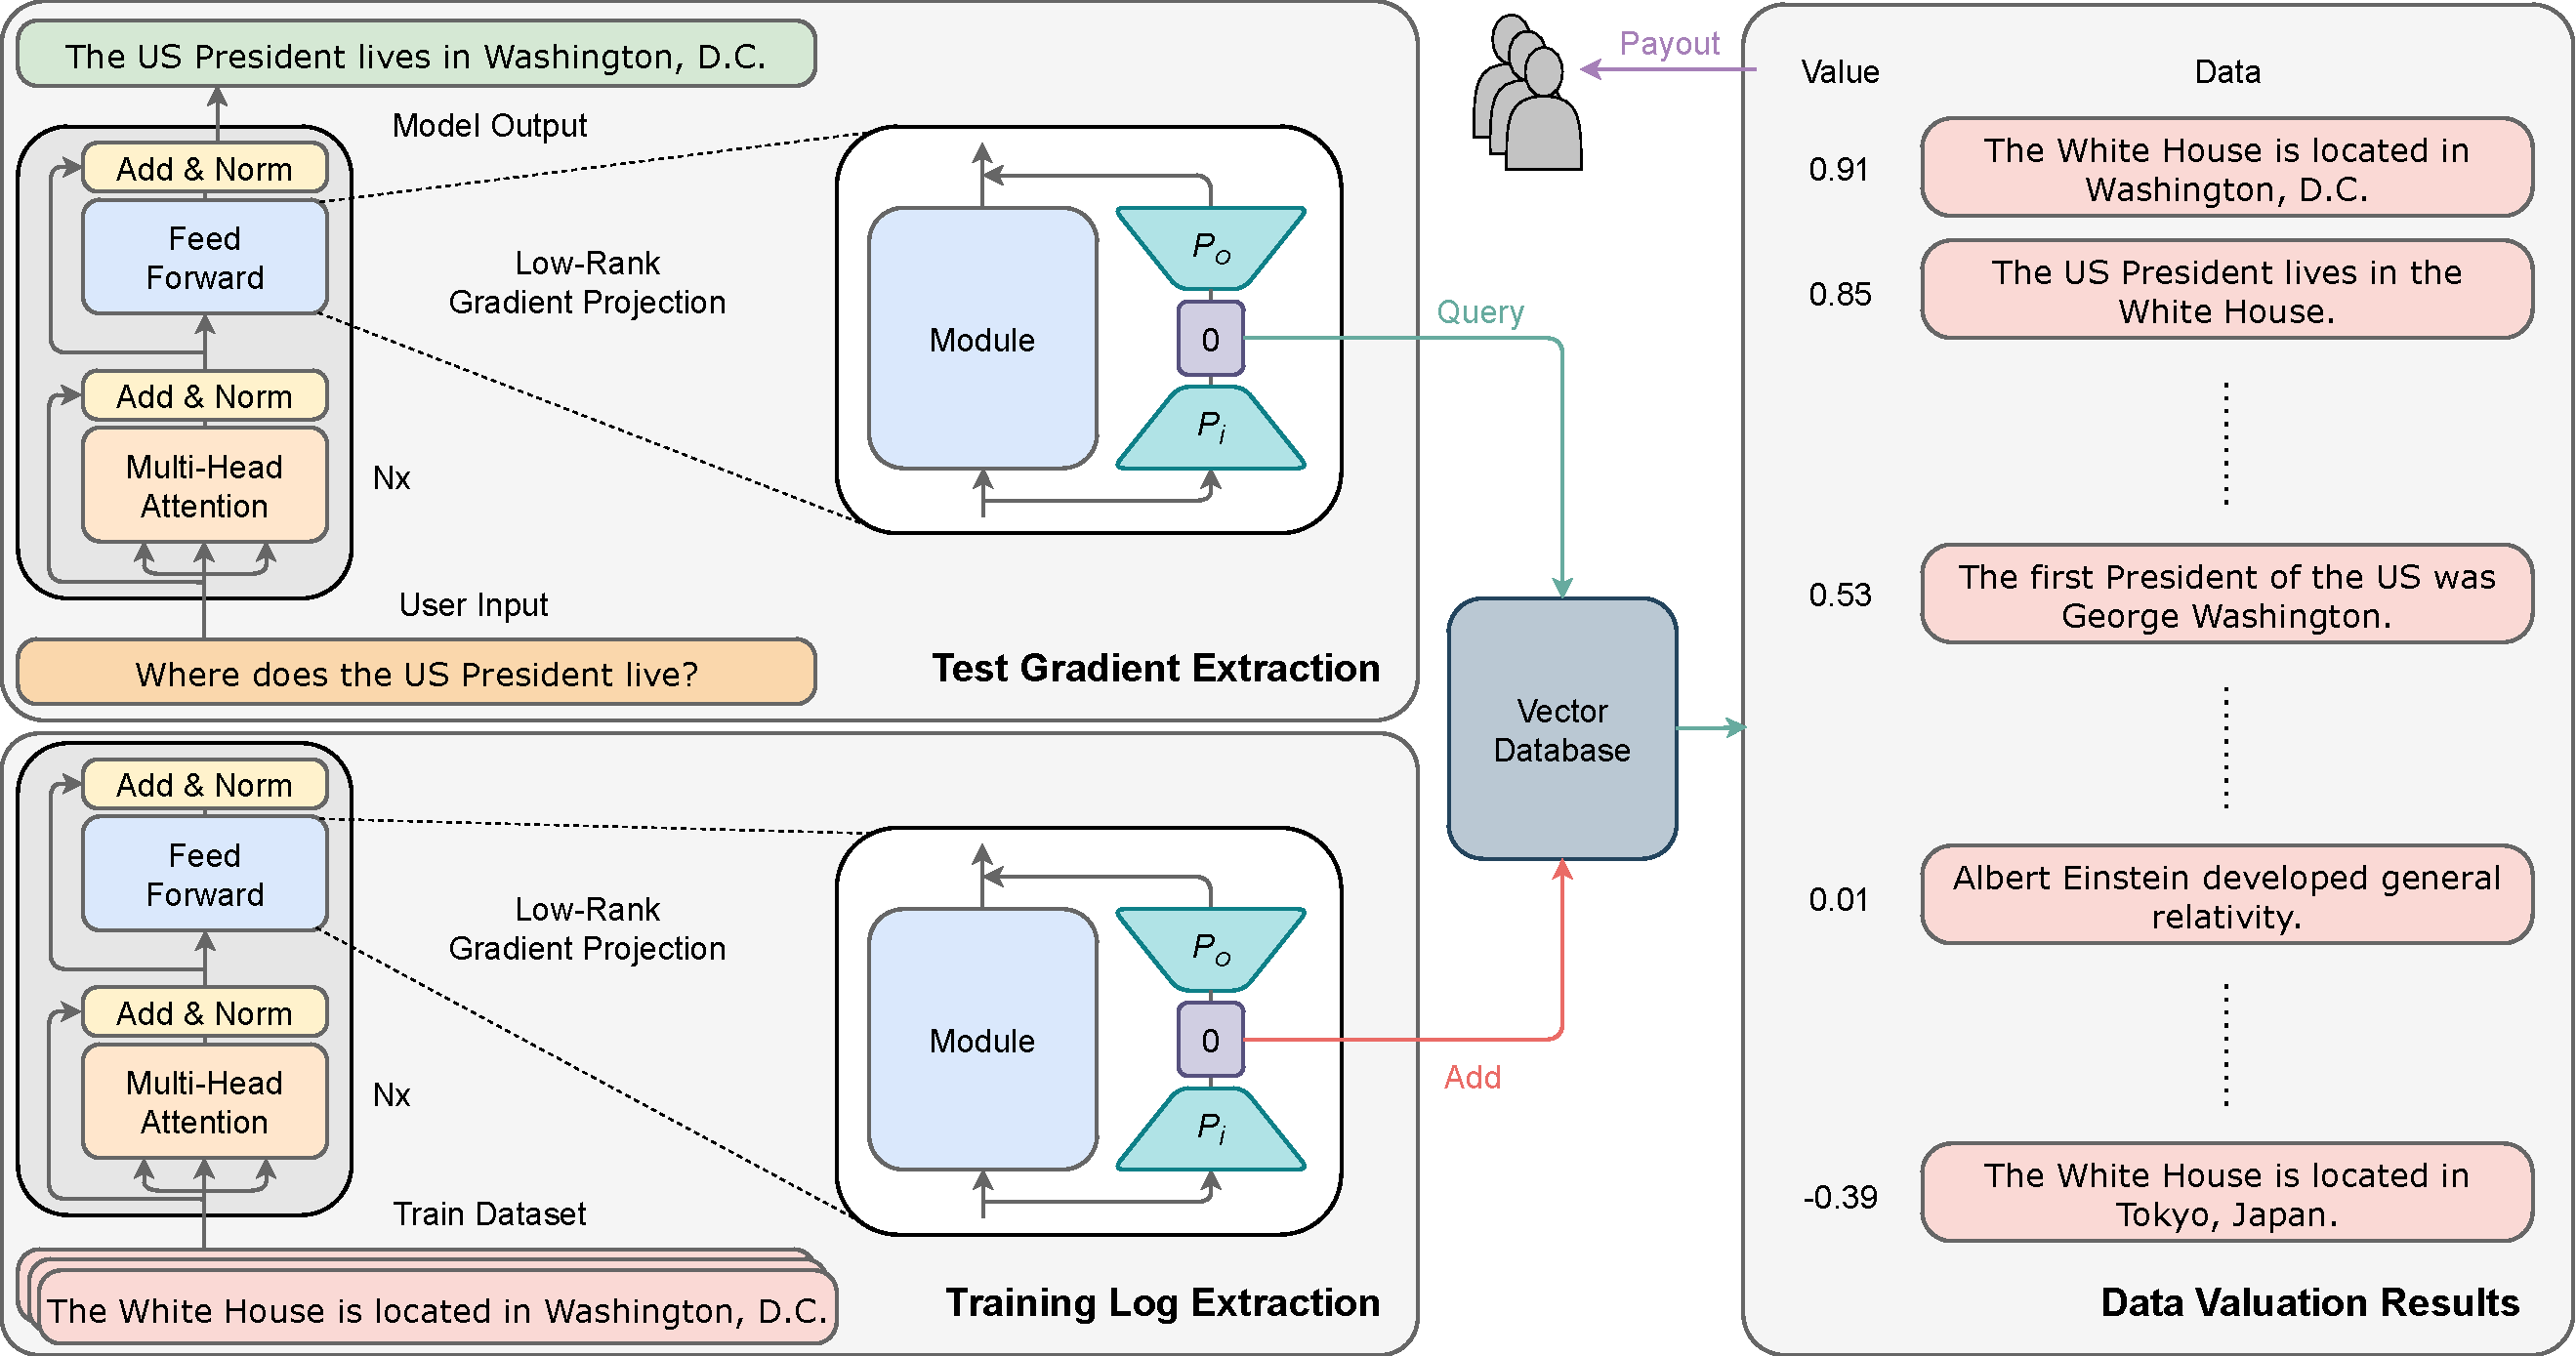
\includegraphics[width=0.94\textwidth]{figures/diagram_v7.pdf}
    \vskip -4pt
    \caption{Data valuation system architecture. \textbf{(Left Bottom)} We first extract the Hessian and gradients for all training data using efficient gradient projection \method\ and store them in a database. \textbf{(Left Top)} At test time, we similarly extract gradients and query the database. \textbf{(Right)} The database returns similarity scores with respect to training examples that can be used for data valuation/attribution.}
    \label{fig:diagram}
\end{figure}

\begin{itemize}[leftmargin=*,topsep=-2pt]
    \item Employing gradient structures in backpropagation, we develop a novel \textbf{lo}w-rank \textbf{gra}dient projection algorithm \method\ that improves space \& time complexity of gradient projection, a major scalability bottleneck in prior work~\cite{park2023trak,schioppa2022scaling}, from $O(nk)$ to $O(\sqrt{nk})$ where $n$ and $k$ are model and projection dimensions. Furthermore, \method\ directly computes projected gradients without materializing full gradients, enabling low GPU memory and high GPU utilization for improved efficiency. Lastly, we show that \method\ can be easily implemented with small add-on layers, similarly to LoRA~\cite{hu2021lora}.
    \item By interpreting a damping term in influence functions as a spectral gradient sparsification mechanism, we (1) offer a theoretical motivation of gradient projection approaches to influence functions and (2) derive a specialized PCA initialization scheme for \method.
    \item We introduce software named \software\ that (1) makes it \textit{simple} to convert existing training code into data valuation code, (2) is \textit{compatible} with various scalability tools and features in the LLM ecosystem, and (3) is \textit{extensible} to implement other data valuation or interpretability algorithms.
    \item In our data valuation experiments, \method\ demonstrates competitive accuracy against more costly baselines, while showing up to 6,500$\times$ increase in throughput and 5$\times$ reduction in GPU memory, when applied to Llama3-8B-Instruct~\cite{llama3modelcard} and the 1B-token dataset, compared to EKFAC influence \cite{grosse2023studying}, the state-of-the-art and only runnable baseline at this scale. We also observe that most valuable data identified by \method\ generally share qualitative similarities with the queried LLM output.
\end{itemize}
\section{Preliminary}
We choose Stable Diffusion (SD) as the base diffusion model in this paper since it is the most popular open-source model and has a well-developed community. SD performs the diffusion process in the latent space of a pre-trained autoencoder.
The input image $I$ is transformed into a latent representation $\boldsymbol{z}_{{0}} = \mathcal{E}(I)$ using a frozen encoder $\mathcal{E}(\cdot)$.
The diffusion process involves applying a variance preserving Markov process to $\boldsymbol{z}_{{0}}$, where noise levels increase monotonically to generate diverse noisy latent representations:
% In training, the encoded image  is perturbed to $\boldsymbol{z}_{{0}}$ by forward diffusion:
\begin{equation}
    \boldsymbol{z}_{{t}}=\sqrt{\bar{\alpha_{t}}} z_{0}+\sqrt{1-\bar{\alpha_{t}}} \epsilon, \epsilon \sim \mathcal{N}(0, I),
\end{equation}
where $t\!=\!1,\cdots, T$ denotes the time steps within the Markov process, where $T$ is commonly configured to 1000, and $\bar{\alpha_{t}}$ represents the pre-defined noise intensity at each time step. 
The denoising network $\epsilon_{\theta}(\cdot)$ learns to reverse this process by predicting the added noise, encouraged by the mean squared error (MSE) loss:
\begin{equation}
    \mathcal{L}=\mathbb{E}_{\mathcal{E}\left(I\right), y, \epsilon \sim \mathcal{N}(0, I), t}\left[\left\|\epsilon-\epsilon_{\theta}\left(z_{t}, t, c_{\mathrm{text}}\right)\right\|_{2}^{2}\right],
\end{equation}
where $c_{\mathrm{text}}$ is the text embedding corresponding to $I$. The denoising network $\epsilon_{\theta}(\cdot)$ is typically implemented as a U-Net~\citep{ronneberger2015unet} consisting of pairs of down/up sample blocks at four resolution levels, as well as a middle block. Each network block consists of ResNet~\citep{he2016deep}, spatial self-attention layers, and cross-attention layers that introduce text conditions.
 \begin{figure*}[h!]
\centering
\small
\tikzset{
    basic/.style  = {draw, text width=2cm, align=center, font=\sffamily, rectangle},
    root/.style   = {basic, rounded corners=2pt, thin, align=center, fill=white,text width=8cm, rotate=90, font=\footnotesize},
    dnode/.style = {basic, thin, rounded corners=2pt, align=center, fill=nblue, text width=7cm, font=\footnotesize},
    dnode_2/.style = {basic, thin, rounded corners=2pt, align=center, fill=nblue, text width=3.5cm, font=\footnotesize},
    dnode_1/.style = {basic, thin, rounded corners=2pt, align=center, fill=nblue, text width=2.5cm, font=\footnotesize}, 
    mnode/.style = {basic, thin, rounded corners=2pt, align=center, fill=ngreen,text width=7cm, font=\footnotesize},
    mnode_2/.style = {basic, thin, rounded corners=2pt, align=center, fill=ngreen,text width=3.5cm, font=\footnotesize},
    mnode_1/.style = {basic, thin, rounded corners=2pt, align=center, fill=ngreen,text width=2.5cm, font=\footnotesize},
    snode/.style = {basic, thin, rounded corners=2pt, align=center, fill=npurple,text width=7cm, font=\footnotesize},
    snode_2/.style = {basic, thin, rounded corners=2pt, align=center, fill=npurple,text width=3.5cm, font=\footnotesize},
    snode_1/.style = {basic, thin, rounded corners=2pt, align=center, fill=npurple,text width=2.5cm, font=\footnotesize},
    dataset_node/.style = {basic, thin, rounded corners=2pt, align=center, fill=nyellow, text width=3.5cm, font=\footnotesize},
    dataset_node_1/.style = {basic, thin, rounded corners=2pt, align=center, fill=nyellow, text width=2.5cm, font=\footnotesize},
    dataset_node_2/.style = {basic, thin, rounded corners=2pt, align=center, fill=nyellow, text width=3.5cm, font=\footnotesize},
    tnode/.style = {basic, thin, align=left, fill=pink!60, text width=15em, align=center},
    xnode/.style = {basic, thin, rounded corners=2pt, align=center, fill=blue!20,text width=5cm,},
    wnode/.style = {basic, thin, align=left, fill=pink!10!blue!80!red!10, text width=6.5em},
    %edge from parent/.style = {draw=black, edge from parent fork right}
    %edge from parent/.style = {draw=black, edge from parent fork down}
}
%
\begin{forest} 
for tree={
    if level=0{
        grow=east,
        growth parent anchor=east,
        parent anchor=south,
        child anchor=west,
        edge path={\noexpand\path[\forestoption{edge},->, >={latex}] 
             (!u.parent anchor) -- +(5pt,0pt) |- (.child anchor)
             \forestoption{edge label};},
    }
    {
        grow=east,
        growth parent anchor=east,
        parent anchor=east,
        child anchor=west,
        edge path={\noexpand\path[\forestoption{edge},->, >={latex}] 
             (!u.parent anchor) -- +(5pt,0pt) |- (.child anchor)
             \forestoption{edge label};},
    }
}
% l sep is used for arrow distance
[KV Cache Management for Large Language Models, root   
    [Datasets and Benchmarks (Sec.~\ref{sec:dataset}), dataset_node_1
        [{Multi-modal Datasets (Sec.~\ref{ssec:multimodal_dataset})}, dataset_node
        ]
        [Text Datasets (Sec.~\ref{ssec:text_dataset}), dataset_node
        ]
    ]
    [System-level Optimization (Sec.~\ref{sec:system-level-opt}), snode_1
        [Hardware-aware Design \\ (Sec.~\ref{sec:sys_hd}), snode_2
            [SSD-based Design (Sec.~\ref{sec:sys_hd_ssd}), snode]
            [Heterogeneous Design (Sec.~\ref{sec:sys_hd_heter}), snode]
            [I/O-based Design (Sec.~\ref{sec:sys_hd_io}), snode]
            [Single/Multi-GPU Design (Sec.~\ref{sec:sys_hd_gpu}), snode]
        ]
        [Scheduling \\ (Sec.~\ref{sec:sys_sch}), snode_2
            [Layer-specific and Hierarchical Scheduling (Sec.~\ref{sec:sys_sch_lhs}), snode]
            [Preemptive and Fairness-oriented Scheduling (Sec.~\ref{sec:sys_sch_pfs}), snode]
            [Prefix-aware Scheduling (Sec.~\ref{sec:sys_sch_ps}), snode]
        ]
        [Memory Management \\ (Sec.~\ref{sec:sys_mm}), snode_2
            [Prefix-aware Design (Sec.~\ref{sec:sys_mm_pd}), snode]
            [Architectural Design (Sec.~\ref{sec:sys_mm_ad}), snode]
        ]
    ]
    [Model-level Optimization (Sec.~\ref{sec:model-level-opt}), mnode_1
        [Non-transformer Architecture (Sec.~\ref{sec:model_nontrans}), mnode_2
            [Hybrid Architecture (Sec.~\ref{sec:model_nontrans_ha}), mnode]
            [Adaptive Sequence Processing Architecture (Sec.~\ref{sec:model_nontrans_na}), mnode]
        ]
        [Architecture Alteration (Sec.~\ref{sec:model_newarch}), mnode_2
            [Augmented Architecture (Sec.~\ref{sec:model_newarch_aug}), mnode]
            [Enhanced Attention (Sec.~\ref{sec:model_newarch_attn}), mnode]
        ]
        [Attention Grouping and Sharing (Sec.~\ref{sec:model_sharing}), mnode_2
            [Cross-Layer Sharing (Sec.~\ref{sec:model_sharing_cross}), mnode]
            [Intra-Layer Grouping (Sec.~\ref{sec:model_sharing_intra}), mnode]
        ]
    ]
    [Token-level Optimization (Sec.~\ref{sec:token_level}), dnode_1
        [KV Cache Low-rank Decomposition  (Sec.~\ref{ssec:kv_low_rank}), dnode_2
            [Learned Low-rank Approximation  (Sec~\ref{sssec:kv_low_rank_learned}), dnode]
            [Tensor Decomposition  (Sec~\ref{sssec:kv_low_rank_tensor}), dnode]
            [Singular Value Decomposition  (Sec~\ref{sssec:kv_low_rank_svd}), dnode]
        ]
         [KV Cache \\Quantization  (Sec.~\ref{ssec:kv_quant}), dnode_2
            [Outlier Redistribution  (Sec~\ref{sssec:outlier_redistribution}), dnode]
            [Mixed-precision Quantization  (Sec~\ref{sssec:kv_quant_mixed_precision}), dnode]
            [Fixed-precision Quantization  (Sec~\ref{sssec:kv_quant_fixed_precision}), dnode]
        ]
        [KV Cache \\Merging  (Sec.~\ref{ssec:kv_merge}), dnode_2
            [Cross-layer Merging  (Sec~\ref{sssec:kv_merge_cross_layer}), dnode]
            [Intra-layer Merging  (Sec~\ref{sssec:kv_merge_intra_layer}), dnode]
        ]
        [KV Cache Budget  Allocation  (Sec.~\ref{ssec:kv_budget}), dnode_2
            [Head-wise Budget Allocation  (Sec~\ref{sssec:kv_budget_head_wise}), dnode]
            [Layer-wise Budget Allocation  (Sec~\ref{sssec:kv_budget_layer_wise}), dnode]
        ]
        [KV Cache \\Selection  (Sec.~\ref{ssec:cache_sel}),dnode_2
            [Dynamic Selection without Permanent Eviction  (Sec~\ref{sssec:dynamic_kv_no_permanent}), dnode]
            [Dynamic Selection with Permanent Eviction  (Sec~\ref{sssec:dynamic_kv_permanent}), dnode]
            [Static KV Cache Selection  (Sec~\ref{sssec:static_kv}), dnode]
        ]
    ]
]
\end{forest}
%\vspace{-1em}
\caption{Taxonomy of KV Cache Management for Large Language Models.}
\label{fig:framework}
\centering

\end{figure*}


\section{Taxonomy}
\label{sec:taxonomy}

In the above sections, we analyzed how the number of cached Key-Value (KV) pairs significantly impacts both the computation time and the additional memory required during inference. Efficient KV cache management is critical to balancing performance improvements and resource utilization, especially as sequence lengths and model sizes continue to grow.
After carefully reviewing existing approaches, we categorize KV cache optimization strategies into three levels: token-level optimization, model-level optimization, and system-level optimizations. 
Each level addresses specific aspects of the challenges associated with KV cache management and offers distinct techniques to enhance efficiency.
The detailed taxonomy is illustrated in  Fig.~\ref{fig:framework}. 
\begin{itemize}[leftmargin=8pt]
    \item \textbf{Token-Level Optimization} refers to improving KV cache management efficiency by focusing on fine-grained  the careful selection, organization, and compression  at the token level, requiring no architectural changes to the original model.    
    While KV cache selection (Sec.~\ref{ssec:cache_sel}) focuses on prioritizing and storing only the most relevant tokens. 
    KV cache budget allocation (Sec.~\ref{ssec:kv_budget}) dynamically distributes memory resources across tokens to ensure efficient cache utilization under limited memory. 
    Furthermore, KV cache merging (Sec.~\ref{ssec:kv_merge}) reduces redundancy by combining similar or overlapping KV pairs, while KV Cache Quantization (Sec.~\ref{ssec:kv_quant}) minimizes the memory footprint by reducing the precision of cached KV pairs. 
    Finally, KV cache low-rank decomposition (Sec.~\ref{ssec:kv_low_rank}) uses  low-rank decomposition technique to reduce cache size.
    
    \item \textbf{Model-level Optimization} refers to designing an efficient model structure to optimize KV cache management. This can further refer to several strategies: Attention grouping and sharing (Sec.~\ref{sec:model_sharing}) methods examine the redundant functionality of key and values and group and share KV cache within or across transformer layers. Architecture alterations (Sec. \ref{sec:model_newarch} emerge to design new attention mechanisms or construct extrinsic modules for KV optimization. Furthermore, there are also works designing or combining non-transformer architectures~\ref{sec:model_nontrans} that adopt other memory efficient designs like recurrent neural networks to optimize the KV cache in traditional transformers. 
    
    \item \textbf{System-level Optimization} refers to optimizing the KV Cache management through two classic low-level aspects: memory management (Sec.~\ref{sec:sys_mm}) and scheduling (Sec.~\ref{sec:sys_sch}). 
    While memory management techniques focusing on architectural innovations like virtual memory adaptation, intelligent prefix sharing, and layer-aware resource allocation, scheduling strategies have evolved to address diverse optimization goals through prefix-aware methods for maximizing cache reuse, preemptive techniques for fair context switching, and layer-specific mechanisms for fine-grained cache control.
    In addition, we provide a detailed introduction for hardware accelerator design in Sec.~\ref{sec:sys_hd}, including single/multi-GPU, I/O-based solutions, heterogeneous computing and SSD-based solutions.
\end{itemize}


\begin{figure*}[t]
\label{fig:kv_cache_summary}
\centering
\tikzset{
    basic/.style  = {draw, text width=2cm, align=center, font=\sffamily, rectangle},
    root/.style   = {basic, rounded corners=2pt, thin, align=center, fill=white,text width=8cm, rotate=90, font=\footnotesize},
    dnode/.style = {basic, thin, rounded corners=2pt, align=center, fill=nblue,text width=3.5cm, font=\footnotesize},
    dnode_1/.style = {basic, thin, rounded corners=2pt, align=center, fill=nblue,text width=2cm, font=\footnotesize},
    dnode_2/.style = {basic, thin, rounded corners=2pt, align=center, fill=nblue,text width=1.7cm, font=\footnotesize},
    mnode/.style = {basic, thin, rounded corners=2pt, align=center, fill=blue!10,text width=3.5cm, font=\footnotesize},
    mnode_1/.style = {basic, thin, rounded corners=2pt, align=center, fill=blue!10,text width=2cm, font=\footnotesize}, 
    snode/.style = {basic, thin, rounded corners=2pt, align=center, fill=npurple,text width=3.5cm, font=\footnotesize},
    snode_1/.style = {basic, thin, rounded corners=2pt, align=center, fill=npurple,text width=2cm, font=\footnotesize},
    tnode/.style = {basic, thin, align=left, fill=pink!60, text width=15em, align=center},
    xnode/.style = {basic, thin, rounded corners=2pt, align=center, fill=blue!20,text width=5cm,},
    wnode/.style = {basic, thin, rounded corners=2pt, align=left, fill=white,text width=5.8cm, font=\footnotesize},
    wnode_1/.style = {basic, thin, rounded corners=2pt, align=left, fill=white,text width=5cm, font=\footnotesize},
    wnode_2/.style = {basic, thin, rounded corners=2pt, align=left, fill=white,text width=6cm, font=\footnotesize},
    %edge from parent/.style = {draw=black, edge from parent fork right}
    %edge from parent/.style = {draw=black, edge from parent fork down}
}
%
\begin{forest} 
for tree={
    grow=east,
    growth parent anchor=east,
    parent anchor=east,
    child anchor=west,
    edge path={\noexpand\path[\forestoption{edge},->, >={latex}] 
         (!u.parent anchor) -- +(5pt,0pt) |- (.child anchor)
         \forestoption{edge label};}
}
% l sep is used for arrow distance
[Token-level Optimization, dnode_2
    [KV Cache Low-rank Decomposition  (Sec.~\ref{ssec:kv_low_rank}), dnode
            [Learned Low-rank Approximation  (Sec~\ref{sssec:kv_low_rank_learned}), dnode
                [   
                    {LESS~\cite{dong2024get},
                    MatryoshkaKV~\cite{linMatryoshkaKVAdaptiveKV2024}
                    }, wnode_1
                ]
            ]
            [Tensor\\ Decomposition  (Sec~\ref{sssec:kv_low_rank_tensor}), dnode
                [
                    {DecoQuant~\cite{liu2024unlocking}
                    }, wnode_1
                ]            
            ]
            [Singular Value Decomposition  (Sec~\ref{sssec:kv_low_rank_svd}), dnode
                [
                    {ECKVH~\cite{yu2024effectively}, EigenAttention~\cite{saxena2024eigen}, 
                    ZDC~\cite{zhang2024zero}, 
                    LoRC~\cite{zhang2024lorc},
                    ShadowKV~\cite{sun2024shadowkv},
                    Palu~\cite{chang2024palu} 
                    }, wnode_1
                ]
            ]
        ]
         [KV Cache \\Quantization  (Sec.~\ref{ssec:kv_quant}), dnode
            [Outlier Redistribution  (Sec~\ref{sssec:outlier_redistribution}), dnode
                [
                {MassiveActivation~\cite{DBLP:journals/corr/abs-2402-17762},
                QuaRot~\cite{ashkboos2024quarot}, Qserve~\cite{DBLP:journals/corr/abs-2405-04532},  Q-INT4~\cite{DBLP:conf/nips/XiLCZ23},
                SpinQuant~\cite{liu2024spinquant},
                DuQuant~\cite{lin2024duquant},
                SmoothQuant~\cite{DBLP:conf/icml/XiaoLSWDH23},
                OS+~\cite{wei2023outlier},
                 AffineQuant~\cite{ma2024affinequant},
                 FlatQuant~\cite{sun2024flatquant},
                 AWQ~\cite{DBLP:conf/mlsys/0002TTYCWXDG024},
                OmniQuant~\cite{shao2023omniquant} }, wnode_1
                ]
            ]
            [Mixed-precision Quantization  (Sec~\ref{sssec:kv_quant_mixed_precision}), dnode
                [
                    {
                    KVQuant~\cite{hooper2024kvquant},
                    IntactKV~\cite{liu2024intactkv},
                    SKVQ~\cite{duanmu2024skvq},
                    KIVI~\cite{liu2024kivi},
                    WKVQuant~\cite{yue2024wkvquant},
                    GEAR~\cite{kang2024gear}, 
                    MiKV~\cite{yang2024no}, 
                    ZIPVL~\cite{he2024zipvl},  ZipCache~\cite{he2024zipcache},
                    PrefixQuant~\cite{chen2024prefixquant},
                    MiniKV~\cite{sharma2024minikvpushinglimitsllm}
                 }, wnode_1
                ]
            ]
            [Fixed-precision Quantization  (Sec~\ref{sssec:kv_quant_fixed_precision}), dnode
                [
                    {ZeroQuant~\cite{yao2022zeroquant},
                    FlexGen~\cite{DBLP:conf/icml/0007ZYLRCLRSZ23}, QJL~\cite{zandieh2024qjl},
                    PQCache~\cite{zhang2024pqcache}
                }, wnode_1
                ]
            ]
        ]
        [KV Cache \\Merging  (Sec.~\ref{ssec:kv_merge}), dnode
            [Cross-layer Merging  (Sec~\ref{sssec:kv_merge_cross_layer}), dnode
            [
            {MiniCache~\cite{DBLP:journals/corr/abs-2405-14366}, KVSharer~\cite{yang2024kvsharerefficientinferencelayerwise}},wnode_1
            ]
            ]
            [Intra-layer \\Merging  (Sec~\ref{sssec:kv_merge_intra_layer}), dnode
                [
                {CCM~\cite{DBLP:conf/iclr/KimYYS24},
                LoMA \cite{wangLoMALosslessCompressed2024},
                {DMC}~\cite{nawrotDynamicMemoryCompression2024}, 
                CaM~\cite{DBLP:conf/icml/0002DLZ00J24}, 
                D2O~\cite{DBLP:journals/corr/abs-2406-13035},
                AIM~\cite{zhong2024aim},
                Look-M~\cite{DBLP:conf/emnlp/WanWLHZJW024},
                KVMerger~\cite{DBLP:journals/corr/abs-2407-08454},
                {CHAI}~\cite{agarwalCHAIClusteredHead2024}}, wnode_1
                ]
            ]
        ]
        [KV Cache Budget  Allocation  (Sec.~\ref{ssec:kv_budget}), dnode
            [Head-wise Budget Allocation  (Sec~\ref{sssec:kv_budget_head_wise}), dnode
                [
                {AdaKV~\cite{DBLP:journals/corr/abs-2407-11550}, CriticalKV~\cite{anonymous2024identify}, LeanKV~\cite{zhang2024unifyingkvcachecompression},
                RazorAttention~\cite{DBLP:journals/corr/abs-2407-15891},
                HeadKV~\cite{DBLP:journals/corr/abs-2410-19258},
                DuoAttention~\cite{DBLP:journals/corr/abs-2410-10819}
                },wnode_1
                ]
            ]
            [Layer-wise Budget Allocation  (Sec~\ref{sssec:kv_budget_layer_wise}), dnode
                [
                {PyramidKV~\cite{DBLP:journals/corr/abs-2406-02069}, PyramidInfer~\cite{DBLP:conf/acl/YangHGHZ024}, 
                DynamicKV~\cite{anonymous2024dynamickv}, PrefixKV~\cite{wang2024prefixkvadaptiveprefixkv},
                SimLayerKV~\cite{DBLP:journals/corr/abs-2410-13846}
                }, wnode_1
                ]
            ]
        ]
    [KV Cache \\Selection  (Sec.~\ref{ssec:cache_sel}),dnode
        [Dynamic Selection without Permanent Eviction  (Sec~\ref{sssec:dynamic_kv_no_permanent}), dnode
            [            {InfLLM~\cite{xiao2024infllmtrainingfreelongcontextextrapolation}, Quest~\cite{DBLP:conf/icml/TangZZXKH24}, PQCache~\cite{zhang2024pqcache}, SqueezedAttention~\cite{hooper2024squeezedattentionacceleratinglong}, RetrievalAttention~\cite{DBLP:journals/corr/abs-2409-10516}, 
            EM-LLM~\cite{DBLP:journals/corr/abs-2407-09450}}, wnode_1
            ]
        ]
        [Dynamic Selection with Permanent Eviction  (Sec~\ref{sssec:dynamic_kv_permanent}), dnode
            [ {H2O~\cite{DBLP:conf/nips/Zhang00CZC0TRBW23}, BUZZ~\cite{zhao2024buzzbeehivestructuredsparsekv}, 
            NACL~\cite{DBLP:journals/corr/abs-2408-03675}, Scissorhands~\cite{DBLP:conf/nips/LiuDLWXXKS23}, Keyformer~\cite{DBLP:conf/mlsys/AdnanAJNSK24},
            SepLLM~\cite{chen2024sepllm}},wnode_1
            ]
        ]
        [Static KV Cache Selection  (Sec~\ref{sssec:static_kv}), dnode
            [{FastGen~\cite{DBLP:conf/iclr/Ge0LZ0024}, SnapKV~\cite{li2024snapkv}, Attention-Gate~\cite{DBLP:journals/corr/abs-2410-12876}},wnode_1
            ]
        ]
    ]
]
\end{forest}

\caption{Taxonomy of the Token-level Optimization for KV Cache Management.}
\label{fig:token_framework}
\end{figure*}

\section{Token-level Optimization }
\label{sec:token_level}
In the token level, optimization focuses exclusively on improving KV cache based on the characteristics and patterns of KV pairs of tokens, without considering enhancements from model architecture improvements or system parallelization techniques.
In general, token-level optimization methods are primarily guided by observations from LLMs and sequential inputs. 
Existing approaches can be categorized into five main types: KV cache selection, KV cache budget allocation, KV cache merging, KV cache quantization, and KV cache low-rank decomposition.
The taxonomy of the token-level optimization is shown in Fig.~\ref{fig:token_framework}.

\subsection{KV Cache Selection}\label{ssec:cache_sel}


KV cache selection mechanisms have emerged as a critical optimization strategy, aimed at reducing memory 
utilization of KV caches, minimizing inference latency, and enhancing overall throughput in large language models. 
These optimization objectives have driven the development of various selection methodologies, which can be 
classified into two distinct categories:
(1) \textbf{static KV cache selection}, which performs token filtering exclusively during the prefilling phase, with selected 
tokens remaining fixed throughout subsequent decoding steps; and (2) \textbf{dynamic KV cache selection}, which continuously 
updates KV cache during the decoding phase, enabling adaptive cache management.
In dynamic KV cache selection approaches, KV cache tokens that are not selected may be permanently evicted or offloaded to hierarchical caching devices such as 
CPU memory, implementing a multi-tier storage strategy. 
Given that real-time KV cache selection during decoding may incur substantial computational overhead, 
several studies have focused on developing optimized retrieval algorithms to enhance the efficiency of 
this process. These optimizations include block-level retrieval instead of token-level granularity to reduce 
search complexity, asynchronous query mechanisms to hide latency, and parallel retrieval pipelines to 
accelerate the selection process. These optimization efforts aim to mitigate the computational burden 
while maintaining the effectiveness of token selection.
The summary of the KV cache selection is listed in Tab.~\ref{tab:kv_cache_summary}.


\begin{table*}[ht]
    \centering
    \caption{Comparison of KV cache selection strategies.}
    \label{tab:kv_cache_summary}
    \renewcommand{\arraystretch}{1.3} % 调整行间距
    \setlength{\tabcolsep}{3pt} % 减小列间距
    \begin{tabular}{lccccccc}
        \toprule
        \textbf{Method} & 
        \makecell{\textbf{Initial}\\\textbf{tokens}} & 
        \makecell{\textbf{Top-$k$}\\\textbf{tokens}} & 
        \makecell{\textbf{Recent}\\\textbf{tokens}} & 
        \makecell{\textbf{Permanent}\\\textbf{eviction}} & 
        \makecell{\textbf{Dynamic}\\\textbf{selection}} & 
        \makecell{\textbf{Selection}\\\textbf{granularity}} & 
        \makecell{\textbf{Remark}} \\ 
        \midrule
        %% Prefilling phase
        FastGen~\cite{DBLP:conf/iclr/Ge0LZ0024} & \checkmark & \checkmark & \checkmark & \checkmark  &  & token & five attention structures\\
        SnapKV~\cite{li2024snapkv} &  & \checkmark & \checkmark & \checkmark &  & token & observation window-based\\
        Attention-Gate~\cite{DBLP:journals/corr/abs-2410-12876} & & \checkmark &  & \checkmark &  & token & learned eviction policy\\
        
        %% Decoding phase
        StreamingLLM~\cite{DBLP:conf/iclr/XiaoTCHL24} & \checkmark & & \checkmark & \checkmark  & \checkmark & token & initial and recent tokens \\
        LM-Infinite~\cite{DBLP:conf/naacl/HanWPX0JW24} & \checkmark  & & \checkmark & \checkmark & \checkmark & token & distance ceiling \\
        H2O~\cite{DBLP:conf/nips/Zhang00CZC0TRBW23} & & \checkmark & \checkmark & \checkmark & \checkmark & token &  accmulative attention score \\
        BUZZ~\cite{zhao2024buzzbeehivestructuredsparsekv} & \checkmark & \checkmark & \checkmark & \checkmark & \checkmark & token &  beehive-like structure \\
        Scissorhands~\cite{DBLP:conf/nips/LiuDLWXXKS23} & & \checkmark & \checkmark & \checkmark  & \checkmark & token & persistence of importance \\
        NACL~\cite{DBLP:journals/corr/abs-2408-03675} & & \checkmark & \checkmark & \checkmark & \checkmark & token & diversified random eviction \\
        Keyformer~\cite{DBLP:conf/mlsys/AdnanAJNSK24} & & \checkmark & \checkmark & \checkmark & \checkmark & token & gumbel logit adjustment \\

        %% block or cluster
        InfLLM~\cite{xiao2024infllmtrainingfreelongcontextextrapolation} & \checkmark & \checkmark & \checkmark &  & \checkmark & block & block-level KV management \\
        Quest~\cite{DBLP:conf/icml/TangZZXKH24} &  & \checkmark &  & & \checkmark & block & new block representation \\
        PQCache~\cite{zhang2024pqcache} & \checkmark  & \checkmark &  \checkmark & & \checkmark & block & product quantization \\
        SqueezedAttention~\cite{hooper2024squeezedattentionacceleratinglong} & & \checkmark & &  & \checkmark & cluster & hierarchical clusters\\
        RetrievalAttention~\cite{DBLP:journals/corr/abs-2409-10516} & \checkmark  & \checkmark & \checkmark &  & \checkmark & cluster & KNN search\\
        EM-LLM~\cite{DBLP:journals/corr/abs-2407-09450} & \checkmark  & \checkmark & \checkmark &  & \checkmark & event & episodic events \\
        
        SparQ~\cite{DBLP:conf/icml/RibarCHBLO24} &  & \checkmark & \checkmark  & & \checkmark & token & low-dimensioanl retrieval\\        
        InfiniGen~\cite{lee2024infinigenefficientgenerativeinference}  &  & \checkmark & & & \checkmark& token & asynchronous prefetching\\
        RecycledAttention~\cite{xu2024recycledattentionefficientinference} & & \checkmark & \checkmark &  & \checkmark & token & periodic top-$k$ selection \\
        MagicPIG~\cite{DBLP:journals/corr/abs-2410-16179} & \checkmark  & \checkmark & \checkmark & & \checkmark & token & Local Sensitive Hash\\

        \bottomrule
    \end{tabular}
\end{table*}

\subsubsection{Static KV Cache Selection}\label{sssec:static_kv}
Static KV cache selection methods perform a one-time compression on the KV Cache 
immediately after the prefilling phase is completed. The model then uses this compressed KV
cache for subsequent decoding inference.
%% FastGen
FastGen~\cite{DBLP:conf/iclr/Ge0LZ0024} introduces a pattern-aware approach by identifying five fundamental attention structures 
and implementing targeted selection strategies. These include proximity-based retention for 
local attention patterns, selective preservation of critical tokens for punctuation-focused 
attention, frequency-based filtering for sparse attention distributions, and complete token 
retention for broad attention patterns.
%% SnapKV
SnapKV~\cite{li2024snapkv} simplifies FastGen's approach by focusing solely on retrieving tokens 
based on their importance scores. It demonstrates that among all prompt tokens, only 
a portion carries crucial information for response generation, with these tokens 
maintaining their significance during the generation phase. The approach employs an 
end-positioned observation window to detect these important contextual tokens. 
Their corresponding key-value pairs are then concatenated with the tokens from the 
observation window.
%% AttentionGate
Attention-Gate~\cite{DBLP:journals/corr/abs-2410-12876} introduces a learnable KV-Cache 
eviction mechanism that processes the entire context sequence and generates token-wise 
eviction decisions through a parameterized policy network, enabling dynamic in-context 
memory management.

\subsubsection{Dynamic Selection with Permanent Eviction}\label{sssec:dynamic_kv_permanent}
This category of methods performs frequent KV cache selection during the decoding phase, 
permanently removing unselected KV cache tokens from memory.
%% StreamingLLM
Early works employ a sliding-window mechanism to address long-text inference challenges, 
where tokens falling outside the window are permanently evicted and become inaccessible.
StreamingLLM~\cite{DBLP:conf/iclr/XiaoTCHL24} uncovers a crucial phenomenon 
in transformer attention where preserved key-value pairs from initial sequence 
tokens maintain crucial model performance. This attention sink effect manifests 
through asymmetric attention weight accumulation at early positions, regardless 
of semantic significance. The approach leverages this characteristic by 
incorporating attention sink positions with recent context for efficient processing.
%% LM-Infinite
LM-Infinite~\cite{DBLP:conf/naacl/HanWPX0JW24} demonstrates that conventional 
techniques, including sliding-window patterns and relative positional encodings, 
fail to resolve length generalization issues. The study introduces a novel methodology 
through the integration of $\Lambda$-shaped attention masking and attention distance 
ceiling mechanisms.

Recent works have explored leveraging attention scores as a criterion for 
selecting significant KV cache tokens.
%% H2O
H2O~\cite{DBLP:conf/nips/Zhang00CZC0TRBW23} observes that attention computations are primarily 
driven by a select group of high-impact tokens, known as Heavy Hitters (H2). This method reformulates 
cache optimization as a dynamic submodular problem, utilizing cumulative attention scores 
to guide token retention decisions.
%% BUZZ
Unlike H2O, BUZZ~\cite{zhao2024buzzbeehivestructuredsparsekv} employs a beehive-like structure that 
selects Heavy Hitters in local KV cache segments.
%% NACL
NACL~\cite{DBLP:journals/corr/abs-2408-03675} identifies a fundamental limitation in H2O, 
namely their dependence on potentially biased local attention statistics. To overcome this issue, 
they develop an alternative approach implementing a diversified random eviction strategy for token 
selection.
%% Scissorhands
Scissorhands~\cite{DBLP:conf/nips/LiuDLWXXKS23} builds upon the temporal significance principle, 
which suggests that tokens demonstrating historical importance maintain their influence in subsequent 
computational steps. This observation enables the preservation of repetitive attention patterns through 
selective token retention.
%% Keyformer
Additionally, Keyformer~\cite{DBLP:conf/mlsys/AdnanAJNSK24} reveals that token removal distorts the underlying softmax probability distribution. 
Considering the pivotal role of softmax distributions in token significance evaluation, 
they incorporate regularization techniques to mitigate these distributional perturbations.
SepLLM~\cite{chen2024sepllm} observes that separator tokens (e.g., commas, periods, and line breaks) receive disproportionately high attention scores and naturally summarize text segments. Building on this, SepLLM retains separator tokens together with initial tokens, important tokens, and recent tokens in the cache.

\subsubsection{Dynamic Selection without Permanent Eviction}\label{sssec:dynamic_kv_no_permanent}

The aforementioned permanent eviction-based approaches face two significant limitations. 
First, the irreversible eviction of tokens potentially impairs the model's performance on 
long-sequence tasks, particularly in needle-in-a-haystack scenarios, and these methods prove 
challenging to adapt to multi-turn dialogue contexts. Second, KV cache selection during the 
decoding phase introduces computational overhead, adversely affecting decoding latency and 
compromising end-to-end acceleration.
%%
To address these challenges, several studies have focused on developing decoding-phase KV 
cache selection strategies without permanent eviction. These approaches typically employ 
multi-tier cache systems (e.g., CPU-GPU hierarchical caching) and leverage advanced data 
structures and system-level enhancements to optimize retrieval efficiency, enabling 
efficient inference with reduced GPU KV cache footprint.


To accelerate the retrieval of critical tokens, several research efforts have proposed 
index-based approaches that organize and access KV cache at block or cluster granularity, 
enabling efficient query and extraction operations.
%% InfLLM: CPU and GPU swap, recent + topk + decoding, block-wise topk
InfLLM~\cite{xiao2024infllmtrainingfreelongcontextextrapolation} maintains full KV cache in blocks while facilitating long sequence 
processing through a hierarchical storage strategy. The framework employs CPU-GPU memory 
orchestration, preserving essential tokens and current computational units in GPU memory 
while offloading less frequently accessed units to CPU memory.
%% Quest
To further enhance top-$k$ block retrieval precision, the Quest~\cite{DBLP:conf/icml/TangZZXKH24} framework presents a refined block representation approach 
based on minimal and maximal key values in KV cache blocks. 
%% PQCache:
PQCache~\cite{zhang2024pqcache} also implements block-based KV cache management and 
identifies salient tokens through Maximum Inner-Product Search (MIPS), leveraging Product 
Quantization (PQ) codes and centroids.
%% SqueezeAttention
SqueezedAttention~\cite{hooper2024squeezedattentionacceleratinglong} employs K-means clustering in an offline stage to group 
semantically similar keys, with each group represented by a centroid. During inference, it compares input queries against these 
centroids to identify and load only the semantically relevant keys from the context.
%% RetrievalAttention
Similarly, RetrievalAttention~\cite{DBLP:journals/corr/abs-2409-10516} index KV cache tokens using approximate
nearest neighbor search (ANNS) techniques.
%% EM-LLM
Additionally, EM-LLM~\cite{DBLP:journals/corr/abs-2407-09450} dynamically segments incoming 
tokens into episodic events. Besides, it implements 
a hybrid retrieval mechanism that combines semantic similarity matching with temporal 
context to efficiently access relevant KV cache segments.




\begin{table*}[t]
    \centering
    \caption{Comparison of KV cache budget allocation strategies.}
    \label{tab:kv_budget_allocation}
    \renewcommand{\arraystretch}{1.3} % 调整行间距
    \setlength{\tabcolsep}{3pt} % 减小列间距
    \begin{tabular}{lcccccc}
        \toprule
        \textbf{Method} & 
        \makecell{\textbf{Layer-wise}} & 
        \makecell{\textbf{Head-wise}} & 
        \makecell{\textbf{Retrieval-head}} & 
        \makecell{\textbf{Input-specific}} & 
        \makecell{\textbf{Extra-calibration}} & 
        \makecell{\textbf{Remark}} \\ 
        \midrule
        PyramidKV~\cite{DBLP:journals/corr/abs-2406-02069} & \checkmark  & & & & &  pyramid-shaped \\
        PyramidInfer~\cite{DBLP:conf/acl/YangHGHZ024} & \checkmark & & & & &  pyramid-shaped \\
        
        DynamicKV~\cite{anonymous2024dynamickv} & \checkmark & & & \checkmark & & maximize attention retention rate \\

        PrefixKV~\cite{wang2024prefixkvadaptiveprefixkv} & \checkmark & & & \checkmark & & maximize attention retention rate \\

        CAKE~\cite{anonymous2024cake} & \checkmark & & & \checkmark & & layer-specific preference score \\
        SimLayerKV~\cite{DBLP:journals/corr/abs-2410-13846} & \checkmark &  &  & \checkmark & & KV cache compression for lazy layers \\

        AdaKV~\cite{DBLP:journals/corr/abs-2407-11550} & & \checkmark & & \checkmark & &  minimize attention computation loss \\
        CriticalKV~\cite{anonymous2024identify} & & \checkmark & & \checkmark & & minimize attention computation loss  \\
        LeanKV~\cite{zhang2024unifyingkvcachecompression} & & \checkmark & & \checkmark & & maximize attention retention rate \\
        RazorAttention~\cite{DBLP:journals/corr/abs-2407-15891} & & \checkmark & \checkmark &  &  \checkmark &  echo and induction heads \\
        HeadKV~\cite{DBLP:journals/corr/abs-2410-19258} & & \checkmark & \checkmark & & \checkmark & retrieval and reasoning heads \\
        DuoAttention~\cite{DBLP:journals/corr/abs-2410-10819} & & \checkmark & \checkmark &  & \checkmark & learned retrieval heads \\
        \bottomrule
    \end{tabular}
\end{table*}

%% SparQ: find r largest components in the query to reduce computation and data transfer
To accelerate top-$k$ token identification, SparQ~\cite{DBLP:conf/icml/RibarCHBLO24} identifies 
the $r$ most significant elements in the incoming query vector and selectively retrieves 
the corresponding components along the hidden dimension of the cached key matrix $K$ for 
approximate attention computation.
%% InfiniGen
To overlap prefetching latency, InfiniGen~\cite{lee2024infinigenefficientgenerativeinference} employs 
asynchronous prefetching, utilizing indices of salient KV entries selected by queries from 
the previous layer to retrieve KV cache entries in the current layer.
%% Recycled Attention
To ensure maximum model performance, RecycledAttention~\cite{xu2024recycledattentionefficientinference} sustains the 
entire KV cache during inference computations, yielding no improvements in memory efficiency. The approach performs periodic top-$k$ token selection to identify salient tokens.
%% MagicPIG
Moreover, MagicPIG~\cite{DBLP:journals/corr/abs-2410-16179} shows that attention-based top-$k$ selection may incur performance degradation. 
To address this limitation, they introduce a novel heterogeneous computing framework leveraging Locality Sensitive Hashing (LSH) techniques. 
The system stores LSH hash tables and performs attention estimation on CPU.

\subsubsection{Summary and Future Directions} 
Static KV cache selection algorithms demonstrate superior decoding efficiency overall; however, 
their efficacy remains to be thoroughly validated in multi-turn dialogues and extended decoding 
length scenarios. Dynamic KV cache selection algorithms, while adaptive, introduce additional 
computational overhead during the decoding phase due to frequent cache selection operations.
Multi-tier cache architectures and prefetching schemes partially mitigate these challenges, 
yet their capability to achieve rapid and accurate retrieval within acceptable decoding latency 
constraints requires further empirical validation, particularly in real-world applications involving 
long sequences. Furthermore, existing selection methods predominantly rely on attention score-based top-$k$ 
selection mechanisms. 
However, based on existing positional encoding schemes, current top-$k$ approaches may not be able to effectively 
identify and extract relevant tokens in ultra-long sequence tasks.







\subsection{KV Cache Budget Allocation} \label{ssec:kv_budget}
The hierarchical architecture of LLMs leads to diverse information extraction patterns across layers, 
with each layer's KV-cache contributing differently to model performance. 
This inherent heterogeneity indicates that uniform KV-cache compression across layers may be suboptimal. 
KV cache budget allocation addresses this challenge by intelligently distributing memory resources based on 
each component's importance to prediction accuracy, thereby optimizing memory utilization while minimizing 
accuracy degradation. Current budget allocation strategies can be categorized into two levels of granularity: 
\textbf{layer-wise} budget allocation, which assigns different compression ratios across model layers, and the more 
fine-grained \textbf{head-wise} budget allocation, which enables precise memory distribution across individual attention 
heads within each layer, offering more flexible and targeted optimization opportunities.
The summary of KV budget allocation is listed in Tab.~\ref{tab:kv_budget_allocation}.




% Please add the following required packages to your document preamble:
% \usepackage{multirow}
\begin{table*}[t]
\renewcommand{\arraystretch}{1.4} % 调整行间距
\centering
\caption{The summary of existing KV Cache merging approaches.}
\label{tab:kv_cache_merging}

\centering
\begin{tabular}{c|cc|c|c|c|c}
\toprule
\multirow{2}{*}{\textbf{Model}} & \multicolumn{2}{c|}{\textbf{Merge Layer}}       & \multirow{2}{*}{\textbf{Merge Unit}} & \multirow{2}{*}{\textbf{Merge Metric}} & \multirow{2}{*}{\textbf{Merge Type}} & \multirow{2}{*}{\textbf{Training-free}} \\ \cline{2-3}
                                & \multicolumn{1}{c|}{\textbf{Intra-layer}} & \textbf{Cross-layer} &                                      &                                         &                                      &                                     \\ \midrule
\textbf{CCM}~\cite{DBLP:conf/iclr/KimYYS24}                    & \multicolumn{1}{c|}{\checkmark}     &       & Token                           & Sliding Window                      & Many-to-One                          & $\times$                              \\

\textbf{LoMA} \cite{wangLoMALosslessCompressed2024} 
   & \multicolumn{1}{c|}{\checkmark}     &       & Token                           & Sliding Window                      & Many-to-Many                          & $\times$              \\

\textbf{DMC}~\cite{nawrotDynamicMemoryCompression2024}                    & \multicolumn{1}{c|}{\checkmark}     &       & Token                           &  Learned Merge Indictor                      & Many-to-One                          & $\times$       \\

\textbf{D2O}~\cite{DBLP:journals/corr/abs-2406-13035}                    & \multicolumn{1}{c|}{\checkmark}     &                & Token                           & Cosine Similarity                      & Two-to-One                           & \checkmark                            \\ 


\textbf{CaM}~\cite{DBLP:conf/icml/0002DLZ00J24}                    & \multicolumn{1}{c|}{\checkmark}               &       &      Token                      & Attention Score                       & Many-to-One                          & \checkmark                                  \\ 



                     
\textbf{AIM}~\cite{zhong2024aim}               & \multicolumn{1}{c|}{\checkmark}     &       & Token                           & Cosine Similarity
                     & Many-to-One                          & \checkmark                                 \\ 

\textbf{Look-M}~\cite{DBLP:conf/emnlp/WanWLHZJW024}               & \multicolumn{1}{c|}{\checkmark}     &       & Token                           & Cosine Similarity
                     & Many-to-One                          & \checkmark                               \\ 

\textbf{KVMerger}~\cite{DBLP:journals/corr/abs-2407-08454}               & \multicolumn{1}{c|}{\checkmark}     &       & Token                           & Weighted Gaussian Kernel
                     & Many-to-One                          & \checkmark                             \\ 
                     
\textbf{CHAI}~\cite{agarwalCHAIClusteredHead2024}               & \multicolumn{1}{c|}{\checkmark}     &       & Head                           & Attention Score
                     & Many-to-One                          & \checkmark                                \\ 


                     
\textbf{MinCache}~\cite{DBLP:journals/corr/abs-2405-14366}               & \multicolumn{1}{c|}{}               & \checkmark      & Token                           & Angular Distance
                    & Two-to-One                       & \checkmark                                \\ 


\textbf{KVSharer}\cite{yang2024kvsharerefficientinferencelayerwise}                & \multicolumn{1}{c|}{}     & \checkmark      & Layer                           & Euclidean distance
                    & Many-to-One     
                         & \checkmark                                \\ \bottomrule
\end{tabular}
\label{tab:merge_comparison}
\end{table*}


\subsubsection{Layer-wise Budget Allocation}\label{sssec:kv_budget_layer_wise}
%% PyramidKV
In contrast to conventional approaches with uniform KV cache sizes, PyramidKV~\cite{DBLP:journals/corr/abs-2406-02069} employs a 
pyramid-shaped memory allocation strategy, assigning larger cache capacities to lower layers that progressively decrease 
in upper layers. This design is supported by the observation that lower layers exhibit uniform attention distributions 
across input sequences, while upper layers show concentrated attention on specific tokens.
%% PyramidInfer
PyramidInfer~\cite{DBLP:conf/acl/YangHGHZ024} also adopts a pyramid-shaped budget allocation strategy while selecting tokens 
with high attention values at each layer. Additionally, during the decoding phase, PyramidInfer dynamically maintains a set of 
significant tokens through frequent updates driven by attention values. 
%% DynamicKV
Unlike previous methods, DynamicKV~\cite{anonymous2024dynamickv} implements an input-adaptive budget allocation strategy by analyzing attention 
patterns. Specifically, it computes the average attention scores between recent and historical tokens, 
identifies the top-$k$ tokens with highest attention values across layers, and proportionally distributes 
the budget based on the density of significant tokens in each layer.
Similarly,
PrefixKV~\cite{wang2024prefixkvadaptiveprefixkv} identifies the most important tokens for each layer by computing the average attention score of tokens within that layer. 
PrefixKV~\cite{wang2024prefixkvadaptiveprefixkv} then uses a unified threshold to determine the number of retained tokens, adaptively adjusting the retention for each layer based on its importance distribution.
%%
CAKE~\cite{anonymous2024cake} examines attention scores through two lenses: the spatial distribution of 
inter-token attention and the temporal evolution of attention focus. These measurements are combined to 
compute layer-specific importance scores, which further guide the allocation of memory resources.
%% SimLayerKV
Additionally, SimLayerKV~\cite{DBLP:journals/corr/abs-2410-13846} identifies lazy layers - 
those exhibiting limited effectiveness in capturing long-range dependencies. 
The framework then selectively preserves cache entries, maintaining  initial and recent tokens 
for lazy layers while retaining complete KV cache for non-lazy layers.



\subsubsection{Head-wise Budget Allocation}\label{sssec:kv_budget_head_wise}
%% Ada-KV
AdaKV~\cite{DBLP:journals/corr/abs-2407-11550} leverages the observation that attention patterns exhibit 
distinct concentrations across different heads. It implements head-specific memory allocation by 
optimizing an L1 loss bound between the original and pruned multi-head attention outputs. 
Within the constraints of a layer-wise budget, the method distributes cache capacity among heads to 
maximize the preserved attention information collectively.
%% CriticalKV
Building upon AdaKV, CriticalKV~\cite{anonymous2024identify} introduces significant enhancements by recognizing that 
the importance of KV cache entries extends beyond attention weights to encompass value states and 
pretrained parameter matrices. Leveraging this insight, the framework implements a novel selection 
algorithm that identifies essential cache entries by minimizing the maximum potential output perturbation.
%% LeanKV
LeanKV~\cite{zhang2024unifyingkvcachecompression} implements a fine-grained memory optimization strategy that operates independently 
for each attention head and input request. The method identifies the smallest subset of tokens 
necessary to preserve the majority of information flow, allocating cache space based on a 
predefined attention score threshold - typically maintaining 95\% of the total attention mass.




%% retrieval head phenomenon
Retrieval head-based methods represent a specialized category of head-wise allocation 
strategies that focuses on identifying and prioritizing attention heads crucial for extracting 
key information from long sequences. This approach allocates larger cache budgets to these 
specialized heads, known as retrieval heads~\cite{DBLP:journals/corr/abs-2404-15574}, due to their 
significant role in information extraction.
%% RazorAttention
RazorAttention~\cite{DBLP:journals/corr/abs-2407-15891} characterizes two distinct categories 
of retrieval heads: echo heads, which focus on previously occurring identical tokens, and induction 
heads, which attend to antecedent tokens that precede current token repetitions. This framework 
implements differential caching strategies, maintaining complete cache entries for retrieval heads 
while condensing remote tokens into consolidated compensation tokens for non-retrieval heads.
%% HeadKV
HeadKV~\cite{DBLP:journals/corr/abs-2410-19258} further enhances RazorAttention by introducing a novel head 
assessment framework that simultaneously evaluates both retrieval and reasoning capabilities to 
optimize KV cache allocation strategies.
%% DuoAttention
DuoAttention~\cite{DBLP:journals/corr/abs-2410-10819} further introduces a parameterized approach to 
distinguish between two categories of attention mechanisms: retrieval heads, essential for comprehensive 
long-context processing, and Streaming heads, which primarily engage with recent tokens and attention 
sinks. This classification is achieved through learned parameters that automatically identify retrieval 
heads requiring full attention spans.



\subsubsection{Summary and Future Directions} 
Despite recent advances and growing attention in KV cache budget allocation research, 
several critical challenges remain unaddressed. First, the relationship between allocation strategies and 
model performance requires further investigation. 
For instance, a notable discrepancy exists between pyramid-shaped allocation 
strategies~\cite{DBLP:journals/corr/abs-2406-02069, DBLP:conf/acl/YangHGHZ024} 
advocating larger budgets for lower layers, and retrieval head-based 
studies~\cite{DBLP:journals/corr/abs-2407-15891,DBLP:journals/corr/abs-2410-19258} 
which demonstrate that lower layers rarely exhibit retrieval head characteristics and 
thus require minimal cache resources. 
Additionally, the field lacks comprehensive experimental comparisons, 
particularly regarding the compatibility and performance benefits of head-wise budget allocation strategies
with state-of-the-art frameworks like vLLM~\cite{DBLP:conf/sosp/KwonLZ0ZY0ZS23} and FlashAttention~\cite{DBLP:conf/nips/DaoFERR22}.
Also,
existing methods, such as PyramidInfer~\cite{DBLP:conf/acl/YangHGHZ024}, demonstrate some adaptability to input attention patterns. However, future research could target real-time, task-specific allocation strategies that dynamically adjust memory budgets during inference based on input characteristics, task complexity, or downstream requirements.





\subsection{KV Cache Merging}\label{ssec:kv_merge}
KV cache merging offers a promising solution by compressing or consolidating KV caches without significantly degrading model accuracy. Rather than a uniform compression strategy, KV cache merging techniques leverage the inherent redundancy within and across layers to dynamically optimize memory utilization. These methods aim to reduce the size of KV caches while preserving critical information necessary for accurate attention computations, enabling efficient inference in resource-constrained settings.
Existing KV cache merging strategies can be categorized into two primary approaches: \textbf{intra-layer merging}, which focuses on consolidating KV caches within individual layers to reduce memory usage per layer, and \textbf{cross-layer merging}, which targets redundancy across layers to eliminate unnecessary duplication. Both approaches offer complementary advantages, providing flexibility to balance memory savings and model performance degradation.
The summary of the KV cache merging is listed in Tab.~\ref{tab:kv_cache_merging}.



\subsubsection{Intra-layer Merging}\label{sssec:kv_merge_intra_layer}
As the input sequence length increases, the number of Keys and Values grows, leading to higher computational costs for the attention process. To address this, CCM~\cite{DBLP:conf/iclr/KimYYS24}, LoMA \cite{wangLoMALosslessCompressed2024}, DMC~\cite{nawrotDynamicMemoryCompression2024} propose to learn a compression module to compress KV of tokens.

Specifically, CCM~\cite{DBLP:conf/iclr/KimYYS24} inserts a special indicator token, \textit{[COMP]}, into the input sequence and compresses the accumulating past attention key/value (KV) pairs in each layer between these indicators into a compact memory space. This compression leverages techniques inspired by the Compressive Transformer~\cite{DBLP:conf/iclr/RaePJHL20} and Gisting~\cite{DBLP:conf/nips/Mu0G23}. 
Instead of computing attention across all tokens, CCM~\cite{DBLP:conf/iclr/KimYYS24} 
computes attention scores for each new token by referencing the merged token. 
Similarly, LoMA~\cite{wangLoMALosslessCompressed2024} inserts a special token into the input sequence to determine which consecutive tokens should be compressed.
LoMA~\cite{wangLoMALosslessCompressed2024} performs compression using bidirectional attention, repetition zone supervision, and carefully designed attention masks and loss functions.
DMC~\cite{nawrotDynamicMemoryCompression2024} learns a variable to decide whether to append new KV pairs to the cache when necessary or to merge them into existing KV representations using a weighted average.
Note that CCM~\cite{DBLP:conf/iclr/KimYYS24}, LoMA~\cite{wangLoMALosslessCompressed2024}, and DMC~\cite{nawrotDynamicMemoryCompression2024} require supervised learning to learn a compression module.



Instead, CaM~\cite{DBLP:conf/icml/0002DLZ00J24}, KVMerger~\cite{DBLP:journals/corr/abs-2407-08454}, and D2O~\cite{DBLP:journals/corr/abs-2406-13035} are training-free, which rely on observations and directly propose rule-based or heuristic-based merging strategies.
Specifically,
they
separate the Keys and Values of tokens in each layer into important (retrained) and unimportant (evicted) tokens. 
They then keep potentially useful unimportant tokens by merging their Keys and Values with  retained important tokens, ensuring that no valuable information is lost.
Particularly, D2O~\cite{DBLP:journals/corr/abs-2406-13035} merges merges  the Key (or Value) of a evicted token with one retained token based on cosine similarity.
Similar to D2O based on cosine similarity, AIM~\cite{zhong2024aim} and Look-M~\cite{DBLP:conf/emnlp/WanWLHZJW024}  merges Keys (resp. Values) of multiple tokens into one.
CaM~\cite{DBLP:conf/icml/0002DLZ00J24} merges  the Keys (or Values) of multiple evicted tokens with  retained tokens based on attention scores to get the final merged results.
Also, KVMerger~\cite{DBLP:journals/corr/abs-2407-08454} first identifies the merge token sets by clustering consecutive tokens with high cosine similarity, ensuring that only adjacent tokens with strong contextual relevance are grouped together. Then, KVMerger merges the tokens in each merge set into the pivotal token (chosen based on the highest attention score) using Gaussian kernel weights, where closer tokens contribute more to the merged state.

Instead of merging the KV of multiple tokens into one, CHAI~\cite{agarwalCHAIClusteredHead2024} observes that heads in multi-head attention often produce highly correlated attention scores for tokens, particularly in the later layers of LLMs. 
To exploit this redundancy, CHAI~\cite{agarwalCHAIClusteredHead2024} clusters attention heads within each layer that produce similar outputs and computes attention for only a single representative head in each cluster.
Specifically, within each cluster, CHAI~\cite{agarwalCHAIClusteredHead2024} selects one representative head to perform the attention computation, and the computed attention scores are shared across all heads in the cluster.




\subsubsection{Cross-layer Merging}\label{sssec:kv_merge_cross_layer}
MiniCache~\cite{DBLP:journals/corr/abs-2405-14366} observes that KV caches in middle-to-deep layers exhibit high angular similarity, making them ideal for merging. 
To achieve this, MiniCache~\cite{DBLP:journals/corr/abs-2405-14366} merges the Key (and Value) pairs of each token from adjacent similar layers into a single shared representation. Specifically,  MiniCache~\cite{DBLP:journals/corr/abs-2405-14366}  decomposes KV vectors into magnitude and direction components, storing only the shared directional vectors, token magnitudes, and unmergeable tokens to maximize memory efficiency.
Differently,
KVSharer~\cite{yang2024kvsharerefficientinferencelayerwise} observes a counterintuitive phenomenon: when the KV caches of two layers differ significantly, sharing one layer's KV cache with another during inference does not cause significant performance degradation. Based on this observation, 
KVSharer~\cite{yang2024kvsharerefficientinferencelayerwise} computes the Euclidean distance between the KV caches of all layer pairs, ranks the pairs by dissimilarity, and prioritizes the most dissimilar layers for sharing.
Since KVSharer~\cite{yang2024kvsharerefficientinferencelayerwise} can share the KV cache of one layer to multiple other layers, the stored KV cache is eliminated significantly.



% Please add the following required packages to your document preamble:
% \usepackage{multirow}
\begin{table*}[t]
\centering
\renewcommand{\arraystretch}{1.5} % 调整行间距

\caption{The summary of existing mixed-precision quantization models.}
\label{tab:kv_mix_precision}

\begin{tabular}{c|cc|ccc|c|c}

\toprule
\multirow{2}{*}{\textbf{Model}} & \multicolumn{1}{c|}{\multirow{2}{*}{\textbf{Keys}}} & \multirow{2}{*}{\textbf{Values}} & \multicolumn{3}{c|}{\textbf{Important Tokens}}                                                & \multirow{2}{*}{\textbf{Outlier storing}} & \multirow{2}{*}{\textbf{Channel Reorder}} \\ \cline{4-6}
                                & \multicolumn{1}{c|}{}                              &                                 & \multicolumn{1}{c|}{\textbf{Intial}} & \multicolumn{1}{c|}{\textbf{Middle}} & \textbf{Recent} &                                   &                                           \\ \hline
\textbf{KVQuant}~\cite{hooper2024kvquant}                & \multicolumn{1}{c|}{Channel, Pre-RoPE}             & Per-Token                           & \multicolumn{1}{c|}{\checkmark}               & \multicolumn{1}{c|}{}                &                 & \checkmark                                 &                                           \\ \hline
\textbf{KIVI}~\cite{liu2024kivi}                   & \multicolumn{1}{c|}{Channel}                       & Per-Token                           & \multicolumn{1}{c|}{}                & \multicolumn{1}{c|}{}                & \checkmark               &                                   &                                           \\ \hline
\textbf{SKVQ}~\cite{duanmu2024skvq}                   & \multicolumn{2}{c|}{Dynamic outlier-aware}                                           & \multicolumn{1}{c|}{\checkmark}               & \multicolumn{1}{c|}{}                & \checkmark               &                                   & \checkmark                                         \\ \hline

\textbf{WKVQuant}~\cite{yue2024wkvquant}               & \multicolumn{2}{c|}{Learnable shifting}                                              & \multicolumn{1}{c|}{}                & \multicolumn{1}{c|}{}                & \checkmark               &                                   &                                           \\ \hline

\textbf{QAQ}~\cite{dong2024qaq}                    & \multicolumn{2}{c|}{Adaptive quantization bits}                                      & \multicolumn{1}{c|}{\checkmark}               & \multicolumn{1}{c|}{\checkmark}               & \checkmark               & \checkmark                                 &                                           \\ \hline
\textbf{MiKV}~\cite{yang2024no}                   & \multicolumn{2}{c|}{Dynamic outlier-aware}                                           & \multicolumn{1}{c|}{\checkmark}               & \multicolumn{1}{c|}{\checkmark}               & \checkmark               &                                   &                                           \\ \hline

\textbf{GEAR}~\cite{kang2024gear}                   & \multicolumn{2}{c|}{Dynamic outlier-aware}                                           & \multicolumn{1}{c|}{}                & \multicolumn{1}{c|}{}                & \checkmark               & \checkmark                                 &                                           \\ \hline
\textbf{ZIPVL}~\cite{he2024zipvl}                  & \multicolumn{2}{c|}{Conventional}                                                    & \multicolumn{1}{c|}{\checkmark}               & \multicolumn{1}{c|}{\checkmark}               & \checkmark               &                                   &                                           \\ \hline
\textbf{CacheGen}~\cite{liu2024cachegen}               & \multicolumn{2}{c|}{Layer-wise, token-locality}                                      & \multicolumn{1}{c|}{}                & \multicolumn{1}{c|}{}                &                 &                                   &                                           \\ \hline
\textbf{Atom}~\cite{zhao2024atom}                   & \multicolumn{2}{c|}{Group-based}                                                     & \multicolumn{1}{c|}{}                & \multicolumn{1}{c|}{}                &                 & \checkmark                                 & \checkmark                                        \\ \bottomrule
\end{tabular}
\end{table*}


\subsubsection{Summary and Future Directions}
KV cache merging represents a transformative approach to optimizing memory utilization in LLMs by consolidating or compressing KV caches while maintaining high model accuracy.
However, there are several key directions and challenges for future exploration in this domain.
Firstly,
current KV cache merging methods are typically designed to work across a wide range of tasks, but fine-tuning merging strategies for specific tasks or domains could further enhance efficiency. For example, certain tasks may tolerate more aggressive merging due to inherent redundancy in their attention patterns, while others may require more conservative approaches to preserve accuracy. Adaptive merging mechanisms that adjust compression levels on-the-fly based on task difficulty, sequence length, or available hardware resources are an exciting avenue for future work.
Secondly,
sparse attention mechanisms, which already reduce the computational complexity of attention by operating on subsets of tokens, could be combined with KV cache merging to achieve even greater efficiency. Exploring how merging complements sparsity-based approaches, such as block-sparse or low-rank attention, could lead to novel hybrid solutions.
Thirdly,
while empirical results show that merging does not significantly degrade performance, providing theoretical guarantees about the preservation of critical information could enhance the reliability of these methods. Future work might focus on quantifying the relationship between merging strategies, token importance, and attention accuracy to provide more formal guarantees.






\subsection{KV Cache Quantization}\label{ssec:kv_quant}
Quantization technique~\cite{lin2016fixed, wu2020integer, kwasniewska2019deep, zhou2018adaptive,jiang2018linear} has been widely used to accelerate machine learning models from different aspects, such model parameter quantization~\cite{frantar2022gptq, dettmers2024qlora, bondarenko2023quantizable,cheng2017quantized} and data feature quantization~\cite{zhou2023dataset,jegou2010product}.
Similarly,
Key-Value (KV) cache quantization is emerging as a highly promising solution to address the memory and computational bottlenecks in LLMs. 
During autoregressive decoding, LLMs generate key-value pairs for every attention layer across all tokens in the sequence. 
If we store all KV pairs in the memory with full precision,
this cache grows exponentially with longer sequences, increasing the memory and bandwidth requirements significantly. 
Quantization reduces the precision of numerical representations (e.g., from FP32 to INT8 or INT4), drastically compressing the size of the KV cache. 
This compression can achieve up to 4x or more memory savings, making it feasible for LLMs to operate on resource-constrained devices like GPUs with limited memory or edge devices.

However, the presence of outliers in Keys and Values poses a significant challenge for low-bit quantization, as these extreme values can lead to substantial performance degradation when compressed into reduced bit representations~\cite{dettmers2022gpt3,bondarenko2021understanding,wei2022outlier}.
Based on the techniques used, existing KV cache quantization approaches can be classified into three main categories: \textbf{Fixed-precision quantization}, where all Keys and Values are quantized to the same bit-width; \textbf{Mixed-precision quantization}, which assigns higher precision to critical parts of the cache while using lower precision for less important components; and \textbf{Outlier redistribution}, which redistributes or smooths the outliers in Keys and Values to improve quantization quality. These methods collectively enable efficient KV cache compression while mitigating the performance degradation typically associated with low-bit quantization.




\subsubsection{Fixed-precision Quantization}\label{sssec:kv_quant_fixed_precision}
Fixed-precision quantization proposes quantizing different Keys (different Values) of tokens to the same bit-width.
ZeroQuant~\cite{yao2022zeroquant} propose per-token quantization for Keys and Values. 
As shown in Fig.~\ref{fig:kv_quant}, the per-token quantization approach quantizes tokens individually.
Particularly, ZeroQuant~\cite{yao2022zeroquant} dynamically computes the min-max range for each token during inference. This ensures that each token is quantized based on its unique range, significantly reducing quantization error.
Also
FlexGen~\cite{DBLP:conf/icml/0007ZYLRCLRSZ23} and QJL~\cite{zandieh2024qjl}  directly perform per-token quantization for Keys and Values, where the scaling factor and zero-point are shared among all elements within the same token.
PQCache~\cite{zhang2024pqcache} uses product quantization approaches~\cite{jegou2010product,matsui2018survey} to compress KV pairs.
However, uniform quantization approaches, which use a fixed bit-width for keys and values across all tokens, can often be suboptimal.
It is because they ignore the varying importance of tokens~\cite{zhang2024unifyingkvcachecompression} and account for the outlier patterns in Keys and Values~\cite{dong2024qaq,hooper2024kvquant}.




 \begin{figure}[t]
    \centering
    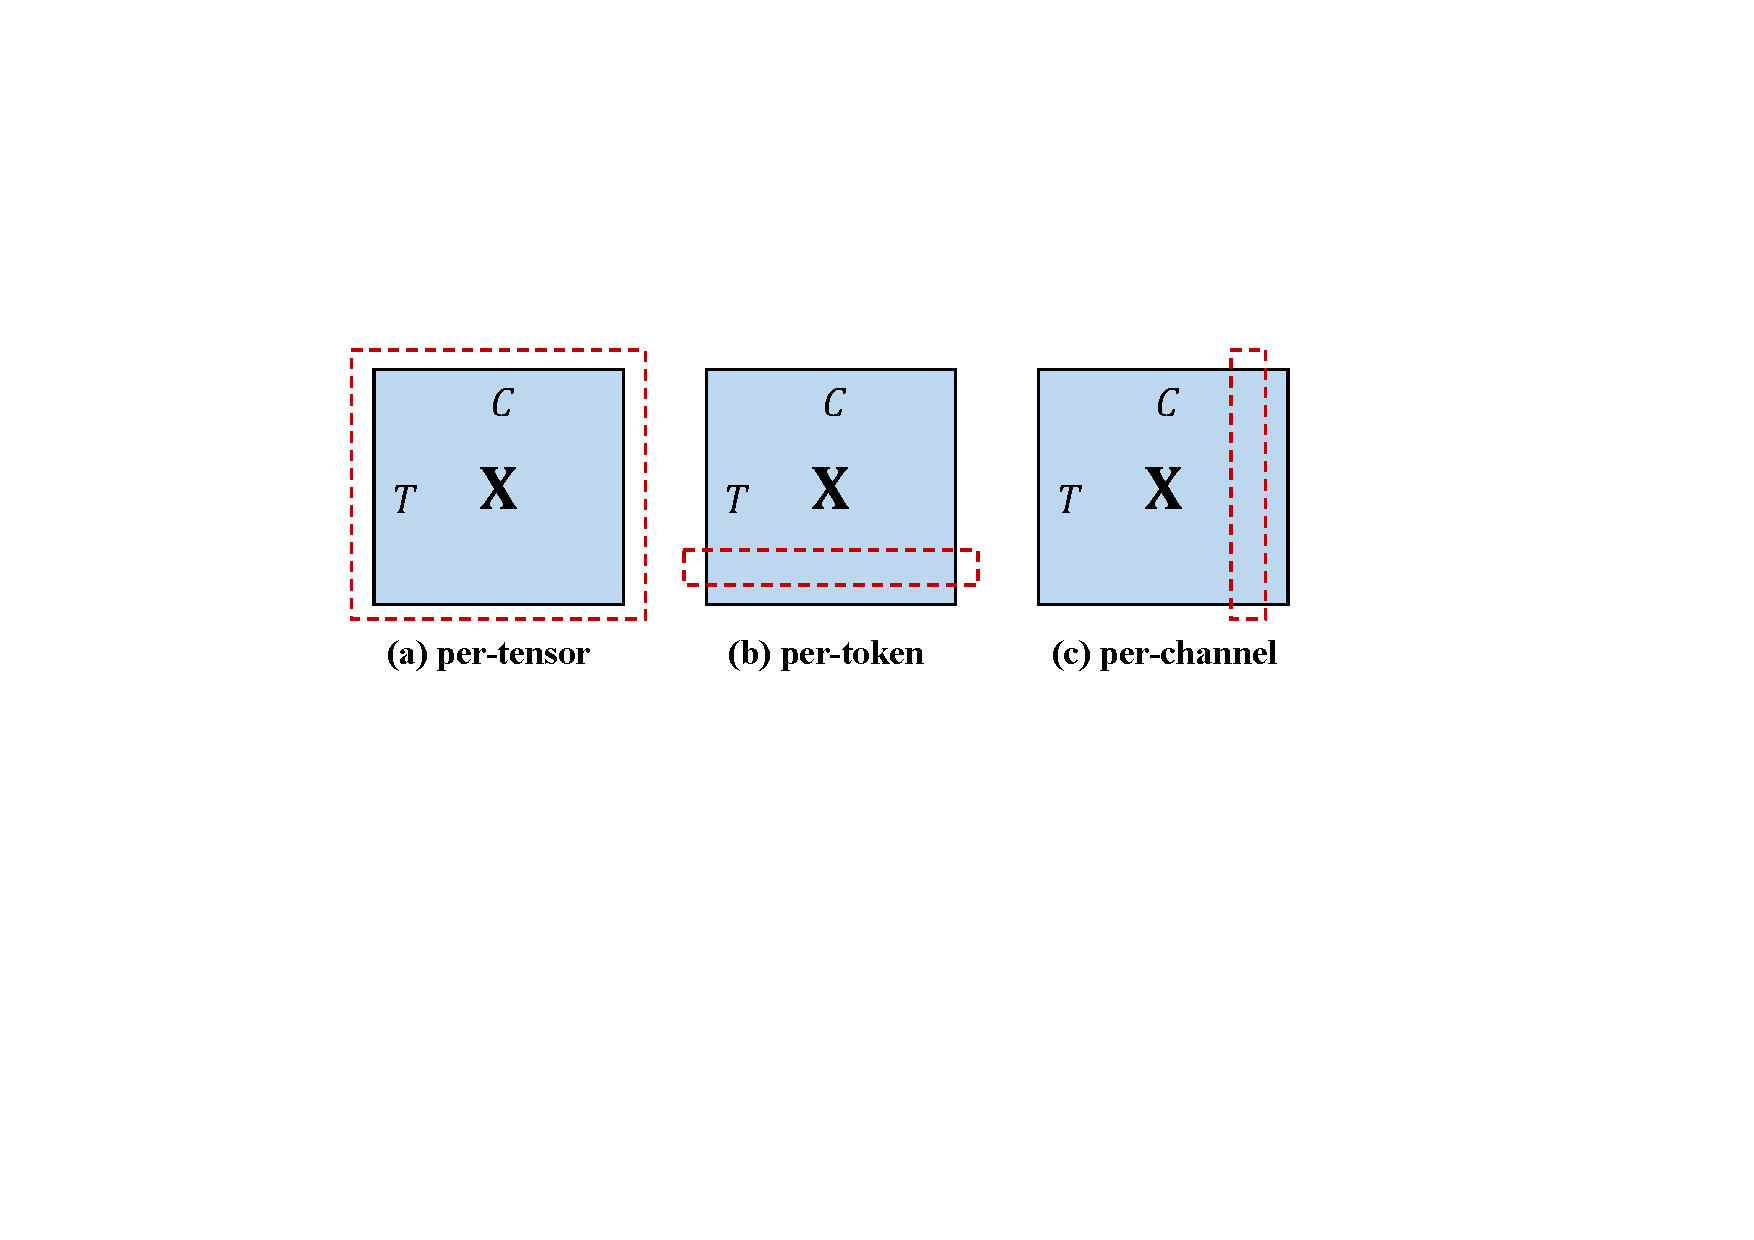
\includegraphics[width=0.88\linewidth]{figures/kv_quant.pdf}
    \caption{Three types of quantization. Then matrix $\mathbf{X} \in \mathbb{R}^{T\times C}$, where $T$ is the number of tokens and $C$ is the feature dimension.}
    \label{fig:kv_quant}
\end{figure}


\subsubsection{Mixed-precision quantization}\label{sssec:kv_quant_mixed_precision}
Unlike fixed-precision quantization, where all Keys or Values are quantized to the same bit-width (e.g., 4-bit or 8-bit), 
mixed-precision quantization assigns higher or full precision to Keys and Values of critical tokens and parts while using lower precision for less critical parts.
The summary of KV mixed-precision quantization is listed in Tab.~\ref{tab:kv_mix_precision}.
KVQuant~\cite{hooper2024kvquant} proposes several strategies to quantize Keys and Values smoothly based on observations.
Firstly, KVQuant observes that the key values exhibit outliers in specific channels prior to applying Rotary Positional Embedding (RoPE).
However, after applying RoPE, the magnitudes of these outlier channels become less consistent, creating a unique challenge for low-precision quantization.
Thus, KVQuant~\cite{hooper2024kvquant} proposes to quantize the Keys per channel before applying the RoPE operations and to quantize the Values per token.
Secondly, KVQuant~\cite{hooper2024kvquant} observes that KV cache activations contain outliers that skew the quantization range. To address this, they isolate outliers per vector (e.g., per-channel or per-token), store them in a sparse format, and quantize the remaining values to a narrower range.
Thirdly, LLMs disproportionately allocate high attention scores to the first token (i.e., attention sink), and quantizing the first token will damage the performance of LLMs.
Thus, KVQuant~\cite{hooper2024kvquant} retains the first token in full precision (FP16) while quantizing the rest of the sequence, which is also used by IntactKV~\cite{liu2024intactkv} and SKVQ~\cite{duanmu2024skvq}.
Similar to KVQuant~\cite{hooper2024kvquant}, KIVI~\cite{liu2024kivi} quantizes the Key cache per-channel, as certain channels exhibit large outliers, and the Value cache per-token,  as there are no significant outlier patterns in the Value cache.
Additionally, KIVI~\cite{liu2024kivi} retains the most recent Keys and Values in full precision, while quantizing older KVs. This approach is based on the observation that the most recent KVs are critical for generating subsequent tokens.


\begin{table*}[t]
\small
\setlength\tabcolsep{2pt}
\centering
\caption{The summary of outlier redistribution models in Sec.~\ref{sssec:outlier_redistribution}.}
\label{tab:outlier_redistribution}
\begin{tabular}{c|c|c|c|c}
\toprule
\textbf{Model} & \textbf{Operation} & \textbf{Formula} & \textbf{Learn} & \textbf{Remarks} \\ \midrule
        MassiveAct.~\cite{DBLP:journals/corr/abs-2402-17762}        &     Add virtual tokens               & $\text{softmax} \left( \frac{\mathbf{Q} \begin{bmatrix} \mathbf{K}^T, & \mathbf{k}' \end{bmatrix}}{\sqrt{d}} \right) 
\begin{bmatrix} \mathbf{V} \\ \mathbf{v}'^T \end{bmatrix}$                 &        \checkmark            &    Learnable $\mathbf{k}'$, $\mathbf{v}'$            \\ \midrule

               
   QuaRot~\cite{ashkboos2024quarot}           &            Hadamard rotation          &  $ \mathbf{XW}^\top = (\mathbf{XH})(\mathbf{H}^\top \mathbf{W}^\top)
$               &          $\times$          &    $\mathbf{H}^\top \mathbf{H} = \mathbf{I}
$             \\ \midrule


   Qserve~\cite{DBLP:journals/corr/abs-2405-04532}            &            Hadamard rotation          &  $ \mathbf{XW}^\top = (\mathbf{XH})(\mathbf{H}^\top \mathbf{W}^\top)
$               &          $\times$          &     $\mathbf{H}^\top \mathbf{H} = \mathbf{I}
$             \\ \midrule


   Q-INT4~\cite{DBLP:conf/nips/XiLCZ23}             &            Hadamard rotation          &  $ \mathbf{XW}^\top = (\mathbf{XH})(\mathbf{H}^\top \mathbf{W}^\top)
$               &          $\times$          &     $\mathbf{H}^\top \mathbf{H} = \mathbf{I}
$             \\ \midrule


               
       SmoothQuant~\cite{DBLP:conf/icml/XiaoLSWDH23}        &     Scaling                &      $  (\mathbf{X} \operatorname{diag}(\mathbf{s})^{-1}) \cdot (\operatorname{diag}(\mathbf{s}) \mathbf{W}^\top)
$            &            $\times$        &    $\mathbf{s} \in \mathbb{R}^{c_i}$              \\ \midrule

               
       QS+~\cite{wei2023outlier}        &    Scaling, Shifting                &      $ ((\mathbf{X}-\mathbf{z}) \operatorname{diag}(\mathbf{s})^{-1} \cdot \operatorname{diag}(\mathbf{s})+\mathbf{z}) \mathbf{W}^\top
$            &         $\times$           &    $\mathbf{s} \in \mathbb{R}^{c_i}$              \\ \midrule


AWQ~\cite{DBLP:conf/mlsys/0002TTYCWXDG024}   &   Scaling                 &       $ \arg\min_{\mathbf{s}} \left\| \mathbf{X}\mathbf{W}^\top - \mathbf{X}\operatorname{diag}(\mathbf{s})^{-1})Q(\operatorname{diag}(\mathbf{s})\mathbf{W}^\top) \right\|$
      &     \checkmark               &  Quantization $Q(\cdot)$                \\ \midrule
      

OmniQuant~\cite{shao2023omniquant}    & Scaling, shifiting                 &   $Q_a\left(\frac{\mathbf{X} - \boldsymbol{\delta}}{\mathbf{s}}\right) Q_w\left(\mathbf{s} \odot \mathbf{W}^\top\right) + \mathbf{B} + \boldsymbol{\delta} \mathbf{W}^\top
$           &       \checkmark               &  Learnable $Q_a(\cdot)$, $Q_w(\cdot)$                 \\ \midrule


      DuQuant~\cite{lin2024duquant}          &        Rotation, permutation            &    $ 
[(\mathbf{X} \cdot \mathbf{\Lambda}) \hat{\mathbf{R}}_{(1)} \cdot \mathbf{P} \cdot \hat{\mathbf{R}}_{(2)}] 
\cdot 
[\hat{\mathbf{R}}_{(2)}^\top \cdot \mathbf{P}^\top \cdot \hat{\mathbf{R}}_{(1)}^\top (\mathbf{\Lambda}^{-1} \cdot \mathbf{W}^\top)]$              &              $\times$      &   Matrices $\mathbf{P}$, $\mathbf{R}$
%permutation and rotation matrices.             
\\ \midrule

    AffineQuant~\cite{ma2024affinequant}           &              Affine transform      &      $\arg\min_{\mathbf{P}} \left\| \mathbf{X}\mathbf{W}^\top - \mathbf{X}\mathbf{P}^{-1} Q(\mathbf{P}\mathbf{W}^\top) \right\|_F^2$            &            \checkmark        &   Quantization $Q(\cdot)$              \\ \midrule

               
    FlatQuant~\cite{sun2024flatquant}    &   Affine transform                  &   AffineQuant +   $\mathbf{P} = \mathbf{P}_1 \otimes \mathbf{P}_2
$            &       \checkmark             & 
Decomposition
%$\operatorname{vec}(\mathbf{V})(\mathbf{P}_1 \otimes \mathbf{P}_2) = \operatorname{vec}(\mathbf{P}_1^\top \mathbf{V} \mathbf{P}_2)$            
\\ \bottomrule        
\end{tabular}
\end{table*}

Similar to KIVI~\cite{liu2024kivi}, WKVQuant~\cite{yue2024wkvquant} temporarily retains the most recent Keys and Values in full precision, while quantizing only the past KV cache. 
This approach helps preserve precision during computation. Additionally, WKVQuant~\cite{yue2024wkvquant} introduces a two-dimensional quantization strategy, which optimizes parameter matrix to align the values in the KV cache into a smoother and more uniform range, significantly improving quantization quality.
GEAR~\cite{kang2024gear}, MiKV~\cite{yang2024no}, ZipCache~\cite{he2024zipcache}  and ZIPVL~\cite{he2024zipvl}  quantize the KV cache based on the importance of each to achieve efficient and effective compression.
First, GEAR~\cite{kang2024gear} applies quantization to compress the majority of less important entries (e.g., 98\%) to ultra-low precision, significantly reducing memory usage. Next, GEAR~\cite{kang2024gear} employs a low-rank matrix to approximate residual errors, capturing structured patterns in the data. Also, GEAR~\cite{kang2024gear} uses a sparse matrix stores outliers, correcting individual errors caused by these values.
MiKV~\cite{yang2024no} is a mixed-precision KV cache quantization approach. Based on the importance of each token, measured using existing methods like H2O~\cite{zhang2023h2o} and SnapKV~\cite{li2024snapkv}, MiKV~\cite{yang2024no} stores less important KV pairs in low precision while retaining the most important KV pairs in high precision.
Instead of approximating the importance weight of each token, ZipCache~\cite{he2024zipcache} accurately computes the importance of each token.
Instead of computing importance score, PrefixQuant~\cite{chen2024prefixquant} observes that token-wise outliers frequently occur at fixed positions (e.g., initial tokens) or low-semantic-value tokens (e.g., ".", "\textbackslash n").
Based on this observation, PrefixQuant~\cite{chen2024prefixquant} identifies high-frequency outlier tokens in LLMs offline and prefixes them in the KV cache, effectively eliminating token-wise outliers.
Similarly, MiniKV~\cite{sharma2024minikvpushinglimitsllm} observes that important tokens can be identified before generation and remain consistent throughout the generation process, retaining these important tokens in high precision.



QAQ~\cite{dong2024qaq} proposes a quality adaptive quantization approach to dynamically determine the suitable quantization bit for each token, based on its importance and sensitivity, while handling outliers and exceptions to maintain model performance.
SKVQ~\cite{duanmu2024skvq} introduces the clipped dynamic quantization with channel reorder. First,  SKVQ~\cite{duanmu2024skvq} uses a transformation-invariant permutation to group similar channels based on their statistical characteristics and applies clipped dynamic quantization to mitigate the outlier problem. Second,  SKVQ~\cite{duanmu2024skvq} maintains high precision for the initial tokens and the most recent tokens while quantizing older tokens. Consequently, SKVQ~\cite{duanmu2024skvq} effectively reduces quantization errors and improves the accuracy of the quantized model.
CacheGen~\cite{liu2024cachegen} and AsymKV~\cite{tao2024asymkv} use layer-wise asymmetric quantization, assigning higher-bit precision  to key matrices in sensitive early layers and lower-bit precision  to less sensitive layers, balancing memory efficiency and performance.
Particularly,
CacheGen~\cite{liu2024cachegen}  also exploits token-wise locality by encoding deltas (differences) between KV tensors of nearby tokens instead of raw values.
Atom~\cite{zhao2024atom} identifies and separates outlier channels, reordering the matrix to group these outlier channels at the end, thereby ensuring regular memory access patterns for improved hardware utilization.
Then, Atom~\cite{zhao2024atom} quantizes outliers with higher precision, while normal channels are quantized to INT4 for maximum efficiency. 
In particular, Atom~\cite{zhao2024atom} applies fine-grained group quantization by dividing matrices into smaller subgroups (e.g., 128 elements per group) and performing quantization independently within each group.







\subsubsection{Outlier Redistribution }\label{sssec:outlier_redistribution}
As previously mentioned, outliers in the Keys and Values present significant challenges for their quantization. Recent research has proposed two main approaches to address this issue: redistributing the outliers into newly appended virtual tokens or applying equivalent transformation functions to smooth the Keys and Values for improved quantization accuracy.
The summary of existing outlier redistribution models are listed in Table.~\ref{tab:outlier_redistribution}.


Specifically, MassiveActivation~\cite{DBLP:journals/corr/abs-2402-17762} highlights the phenomenon of massive activations in large language models (LLMs), where a small subset of activations is exponentially larger than the rest. To address this, MassiveActivation~\cite{DBLP:journals/corr/abs-2402-17762} proposes appending a virtual token to the inputs, allowing LLMs to encapsulate the massive outliers within these learned keys and values for each head.
Then, we introduce the  equivalent transformation function-based approaches. Firstly,
QuaRot~\cite{ashkboos2024quarot}, Qserve~\cite{DBLP:journals/corr/abs-2405-04532}, and Q-INT4~\cite{DBLP:conf/nips/XiLCZ23} redistributes outlier values across all channels by Hadamard rotation, successfully lowering the maximum value of outlier tokens. 
The Hadamard rotation of activations can be incorporated into the preceding linear layer, thereby redistributing the outliers of Keys and Values into the parameters.
Despite this improvement, outlier tokens still exhibit magnitudes hundreds of times greater than normal tokens, causing notable performance issues when using shared quantization scales across tokens~\cite{chen2024prefixquant}.
Expanding on this idea, SpinQuant~\cite{liu2024spinquant} proposes training an orthogonal matrix instead of relying on a random Hadamard matrix to achieve better performance. Similarly, DuQuant~\cite{lin2024duquant} employs channel permutation to evenly distribute outliers across blocks and utilizes block rotation to further smooth outliers.  



SmoothQuant~\cite{DBLP:conf/icml/XiaoLSWDH23} leverages a key observation that different tokens show similar patterns of variation across their channels. Based on this insight, it strategically shifts the quantization complexity from activations to weights through an offline process.
Specifically, SmoothQuant~\cite{DBLP:conf/icml/XiaoLSWDH23} introduces a mathematically equivalent per-channel scaling transformation:
$\mathbf{Y} = (\mathbf{X}\text{diag}(\mathbf{s})^{-1}) \cdot (\text{diag}(\mathbf{s})\mathbf{W}) = \mathbf{\hat{X}}\mathbf{\hat{W}}$
where $\mathbf{X}$ represents Keys or Values, and the smoothing factor $\mathbf{s}\in \mathbb{R}^{C_i}$ is used to scale $\mathbf{X}$. This transformation achieves two key benefits: it smooths the distribution of Keys and Values to facilitate easier quantization, and it allows the smoothing factors to be efficiently incorporated into the parameters of previous layers during offline processing.
In particular, the smooth factor $\mathbf{s}$ is dynamically decided on based on inputs.
Similarly,
The OS+~\cite{wei2023outlier} introduces channel-wise shifting to eliminate outlier asymmetry and channel-wise scaling to reduce outlier concentration. These operations are seamlessly migrated to subsequent layers, maintaining equivalence with the floating-point model while improving quantization performance.
%DuQuant~\cite{lin2024duquant}ntroduces a dual transformation approach using rotation and permutation matrices to redistribute activation outliers for efficient quantization.



Instead of using handcrafted transformations~\cite{lin2024duquant,wei2023outlier,DBLP:conf/icml/XiaoLSWDH23} to shift the quantization difficulty from activations to weights,
AffineQuant~\cite{ma2024affinequant}
uses an affine transformation matrix that combines both scaling and rotation transformations. 
This allows it to optimize weight distributions more effectively, aligning them better with the quantization function and reducing quantization errors.
The affine transformation matrix provides richer flexibility compared to SmoothQuant’s scalar-based scaling, enabling finer adjustments to the weight and activation distributions.
Based on AffineQuant~\cite{ma2024affinequant},
FlatQuant~\cite{sun2024flatquant} introduces a fast and learnable affine transformations to enhance the flatness of weights and activations, which decomposes transformations into smaller matrices to reduce memory and computational costs.
Similarly,
AWQ~\cite{DBLP:conf/mlsys/0002TTYCWXDG024} and 
OmniQuant~\cite{shao2023omniquant} proposes
differentiable and learnable equivalent transformations, 
which optimize the equivalent parameters (e.g., channel-wise scaling and shifting) in an end-to-end manner using gradient descent.

\subsubsection{Summary and Future Directions}
KV cache quantization is a crucial technique for reducing memory and computational overhead in large language models (LLMs) during autoregressive decoding. While significant progress has been made, this field remains dynamic and rapidly evolving, with several promising directions for future research.
Firstly,
one promising avenue is the development of real-time adaptive quantization methods. These techniques could dynamically adjust quantization levels during inference based on real-time metrics such as token importance, outlier presence, or sequence length. Such an approach could significantly enhance efficiency while maintaining performance, especially for processing long sequences with varying levels of complexity.
Secondly,
another important direction is extending KV cache quantization to multi-modal and multi-task models. Multi-modal models, which process inputs from diverse domains such as text, vision, and audio, and multi-task scenarios often exhibit highly diverse attention patterns and memory demands. This necessitates the design of more advanced and tailored quantization strategies to balance efficiency and accuracy in these increasingly complex settings.

Thirdly,
hybrid quantization techniques also hold significant potential. By combining fixed-precision, mixed-precision, and outlier redistribution methods, researchers could develop more versatile and efficient quantization frameworks. For instance, integrating mixed-precision allocation schemes with outlier smoothing transformations could optimize both memory usage and performance, offering a flexible approach adaptable to a variety of tasks and models.
finally, addressing the challenge of outliers remains a critical area of focus. Outliers can have a disproportionate impact on quantization efficiency and model performance. Future research could explore advanced outlier detection mechanisms or innovative encoding techniques to mitigate their effects. Improved handling of outliers could further enhance the effectiveness of quantization methods, enabling more robust and memory-efficient implementations.




\subsection{KV Cache Low-rank Decomposition}\label{ssec:kv_low_rank}
Existing studies have demonstrated that the majority of information within KV caches can be captured by a small subset of their singular values or low-rank components, making low-rank decomposition a powerful tool for compression. 
By leveraging this property, KV cache low-rank decomposition techniques aim to reduce memory requirements while preserving the essential information required for accurate attention computations.
Low-rank decomposition strategies can be classified into three main approaches: \textbf{Singular Value Decomposition (SVD)}, which exploits the low-rank structure of KV matrices to retain the most critical singular values; 
\textbf{Tensor Decomposition}, which factorizes KV matrices into smaller components for minimal redundancy; 
and \textbf{Learned Low-rank Approximation}, which incorporates adaptive mechanisms to optimize compression based on learned representations. 
Each method provides a unique balance of computational efficiency and accuracy retention, enabling scalable and memory-efficient LLM inference.



\subsubsection{Singular Value Decomposition}\label{sssec:kv_low_rank_svd}
Firstly, 
ECKVH~\cite{yu2024effectively}, EigenAttention~\cite{saxena2024eigen}, and ZDC~\cite{zhang2024zero} shows that KV caches have a low-rank property, where a small number of top singular values retain most of the information. Using Singular Value Decomposition (SVD), the method compresses KV caches by grouping heads, applying SVD, and retaining top singular values, effectively reducing the number of KV heads with minimal error.
Also, ZDC~\cite{zhang2024zero} uses an adaptive hybrid compression ratio mechanism to assign higher compression to unimportant tokens in shallower layers while preserving more important tokens in deeper layers, leveraging the similarity of token characteristics in adjacent layers.
Secondly, rather than decomposing KV pairs, LoRC~\cite{zhang2024lorc} employs a low-rank approximation of KV weight matrices and adopts a progressive compression strategy to efficiently compress KV caches without requiring model retraining.
Specifically,
LoRC~\cite{zhang2024lorc} uses SVD to compress the Keys and Values parameter matrices (i.e., $\mathbf{W}^k_i$ and $\mathbf{W}^v_i$) as  $\mathbf{W}^k_i=\mathbf{U}^k_i \mathbf{\Sigma}^k_i {\mathbf{P}^k_i}^\top$ and $\mathbf{W}^v_i=\mathbf{U}^v_i \mathbf{\Sigma}^v_i {\mathbf{P}^v_i}^\top$.
Also, compression is applied conservatively in shallower layers to minimize error amplification and more aggressively in deeper layers.
Then, instead of storing $\mathbf{K}^i=\mathbf{X}_i\mathbf{W}^k_i$ and $\mathbf{V}^i=\mathbf{X}_i\mathbf{W}^v_i$, it only stores $\mathbf{\hat{K}}^i=\mathbf{X}_i\mathbf{U}^k_i$ and $\mathbf{\hat{V}}^i=\mathbf{X}_i\mathbf{U}^v_i$, along with $ \mathbf{\Sigma}^k_i {\mathbf{P}^k_i}^\top$ and $ \mathbf{\Sigma}^v_i {\mathbf{P}^v_i}^\top$.
Also, ShadowKV~\cite{sun2024shadowkv} performs SVD decomposition directly on pre-RoPE keys to reduce the dimensionality of the key representations.
Palu~\cite{chang2024palu} applies SVD to compress both Keys and Values.





\subsubsection{Tensor Decomposition}\label{sssec:kv_low_rank_tensor}
Tensor decomposition~\cite{kuleshov2015tensor, zhou2017tensor,haeffele2015global} is a widely used algorithm for factorizing a matrix into a sequential product of local tensors, such as Matrix Product Operator (MPO)~\cite{liu2021enabling} and turker decomposition~\cite{malik2018low} .
Taking Matrix Product Operator (MPO)~\cite{liu2021enabling} as an example, the decomposition of a matrix $\mathbf{W} \in \mathbb{R}^{I \times J}$ using MPO can be  defined as:
\begin{equation}\label{eq:mpo}
    \text{TD}(\mathbf{W}) = \prod_{k=1}^n \mathcal{T}_{(k)}[d_{k-1}, i_k, j_k, d_k],
\end{equation}
where $\mathcal{T}_{(k)}$ represents the local tensor of size $d_{k-1} \times i_k \times j_k \times d_k$, with $\prod_{k=1}^n i_k = I$ and $\prod_{k=1}^n j_k = J$. Here, $n$ denotes the number of local tensors, collectively referred to as the decomposed tensors.
As shown in Eaquation~\eqref{eq:mpo},
MPO-based tensor decomposition is well-suited for KV cache compression as it reduces the memory footprint by factorizing large key and value matrices into smaller local tensors, enabling efficient storage while preserving essential information. This approach minimizes redundancy and maintains the structural integrity required for accurate attention computations.
DecoQuant~\cite{liu2024unlocking} combines quantization with low-rank decomposition to effectively reduce quantization errors. Specifically, DecoQuant~\cite{liu2024unlocking} leverages the Matrix Product Operator (MPO) to decompose matrices into smaller local tensors. The larger tensors, which contain most of the parameters, are quantized to low-bit precision, while the smaller tensors retain high precision to minimize overall quantization error.

\subsubsection{Learned Low-rank Approximation}\label{sssec:kv_low_rank_learned}
LESS~\cite{dong2024get} introduces a novel {learned-kernel-based low-rank approximation} approach to efficiently approximate the results of the softmax function. Specifically, LESS~\cite{dong2024get} replaces the softmax with a {separable similarity metric}, \(\phi(\mathbf{q}_t) \psi(\mathbf{K}_t)^\top\), where \(\phi\) and \(\psi\) are row-wise functions. Here, \(\mathbf{q}_t \in \mathbb{R}^{1 \times D}\) represents the query, and \(\mathbf{K}_t \in \mathbb{R}^{t \times D}\) represents the keys at step \(t\).
To elaborate, if \(\phi\) and \(\psi\) are such that:
$a_t = \text{softmax} \left( \frac{\mathbf{q}_t \mathbf{K}_t^\top}{\sqrt{D}} \right) \mathbf{V}_t 
\approx \frac{\phi(\mathbf{q}_t) \psi(\mathbf{K}_t)^\top \mathbf{V}_t}{\phi(\mathbf{q}_t) \psi(\mathbf{K}_t)^\top \mathbf{1}_{S \times 1}}$,
then we only need to cache the {hidden states} \(\mathbf{H}_t = \psi(\mathbf{K}_t)^\top \mathbf{V}_t \in \mathbb{R}^{R \times D}\) and the {normalization factor} \(\mathbf{z}_t = \sum_{s=1}^t \psi([\mathbf{K}_t]_s) \in \mathbb{R}^{1 \times R}\) for inference.
Similarly,
MatryoshkaKV~\cite{linMatryoshkaKVAdaptiveKV2024} 
compresses KV caches along the feature dimension by leveraging trainable orthogonal projection matrices.


\subsubsection{Summary and Future Directions}
KV cache low-rank decomposition is a powerful technique for compressing KV caches in LLMs while maintaining the quality of attention computations. Current methods primarily rely on fixed low-rank approximations applied uniformly across all layers or tokens. However, future advancements could focus on dynamic rank adjustment, where the rank is tailored based on token importance, sequence length, or layer-specific properties, enabling a more optimal balance between memory efficiency and performance.
Additionally, real-time or streaming applications present a promising avenue for exploration. Since KV caches grow dynamically during inference, lightweight and incremental decomposition methods that can adapt efficiently to expanding sequences will be critical for supporting such scenarios without compromising latency or accuracy.





 

%\todo{整体check表格}

\section{Model-level Optimization}\label{sec:model-level-opt}
% {\color{red}please check this paper whther in this level: Lossless KV Cache Compression to 2\% (already included: CLLA)}
\begin{figure*}[t]
\centering
\tikzset{
    basic/.style  = {draw, text width=2cm, align=center, font=\sffamily, rectangle},
    root/.style   = {basic, rounded corners=2pt, thin, align=center, fill=white,text width=8cm, rotate=90, font=\footnotesize},
    dnode/.style = {basic, thin, rounded corners=2pt, align=center, fill=ngreen, text width=3.5cm, font=\footnotesize},
    dnode_1/.style = {basic, thin, rounded corners=2pt, align=center, fill=ngreen,text width=2cm, font=\footnotesize},
    mnode/.style = {basic, thin, rounded corners=2pt, align=center, fill=ngreen,text width=3.5cm, font=\footnotesize},
    mnode_1/.style = {basic, thin, rounded corners=2pt, align=center, fill=ngreen,text width=2.5cm, font=\footnotesize}, 
    mnode_2/.style = {basic, thin, rounded corners=2pt, align=center, fill=ngreen,text width=2.5cm, font=\footnotesize}, 
    snode/.style = {basic, thin, rounded corners=2pt, align=center, fill=green!30,text width=3.5cm, font=\footnotesize},
    snode_1/.style = {basic, thin, rounded corners=2pt, align=center, fill=green!30,text width=2.5cm, font=\footnotesize},
    tnode/.style = {basic, thin, align=left, fill=pink!60, text width=15em, align=center},
    xnode/.style = {basic, thin, rounded corners=2pt, align=center, fill=blue!20,text width=5cm,},
    wnode/.style = {basic, thin, rounded corners=2pt, align=left, fill=white,text width=5cm, font=\footnotesize},
    %edge from parent/.style = {draw=black, edge from parent fork right}
    %edge from parent/.style = {draw=black, edge from parent fork down}
}
%
\begin{forest} 
for tree={
    grow=east,
    growth parent anchor=east,
    parent anchor=east,
    child anchor=west,
    edge path={\noexpand\path[\forestoption{edge},->, >={latex}] 
         (!u.parent anchor) -- +(5pt,0pt) |- (.child anchor)
         \forestoption{edge label};}
}
% l sep is used for arrow distance
[Model-level \\Optimization (Sec.~\ref{sec:model-level-opt}), mnode
    [Non-transformer Architecture (Sec.~\ref{sec:model_nontrans}), mnode
        [Hybrid Architecture (Sec.~\ref{sec:model_nontrans_ha}), mnode
            [{MixCon \cite{xuMixConHybridArchitecture2024},
            GoldFinch \cite{goldsteinGoldFinchHighPerformance2024},
            RecurFormer \cite{yanRecurFormerNotAll2024}}, wnode]
        ]
        [Adaptive Sequence Processing Architecture (Sec.~\ref{sec:model_nontrans_na}), mnode
            [{RWKV \cite{pengRWKVReinventingRNNs2023},
            Mamba \cite{guMambaLinearTimeSequence2024},
            RetNet \cite{sunRetentiveNetworkSuccessor2023},
            MCSD \cite{yangMCSDEfficientLanguage2024}}, wnode]
        ]
    ]
    [Architecture Alteration (Sec.~\ref{sec:model_newarch}), mnode
        [Augmented \\Architecture (Sec.~\ref{sec:model_newarch_aug}), mnode
            [{YOCO \cite{sunYouOnlyCache2024}, 
            CEPE \cite{yenLongContextLanguageModeling2024a}, 
            XC-Cache \cite{monteiroXCCacheCrossAttendingCached2024}, 
            Block Transformer \cite{hoBlockTransformerGlobaltoLocal2024}}, wnode]
        ]
        [Enhanced Attention (Sec.~\ref{sec:model_newarch_attn}), mnode
            [{
            MLA \cite{deepseek-aiDeepSeekV2StrongEconomical2024},
            FLASH \cite{huaTransformerQualityLinear2022}, 
            Infini-Attention \cite{munkhdalaiLeaveNoContext2024}}, wnode]
        ]
    ]
    [Attention Grouping and Sharing (Sec.~\ref{sec:model_sharing}), mnode
        [Cross-Layer Sharing (Sec.~\ref{sec:model_sharing_cross}), mnode
            [{CLA \cite{brandonReducingTransformerKeyValue2024}, 
            LCKV \cite{wuLayerCondensedKVCache2024}, 
            SA  \cite{liaoKVCachingShared2024},
            MLKV \cite{zuhriMLKVMultiLayerKeyValue2024},
            LISA \cite{muCrosslayerAttentionSharing2024},
            Wu et al. \cite{wuSystematicStudyCrossLayer2024},
            CLLA \cite{yangLosslessKVCache2024},
            DHA \cite{chenDHALearningDecoupledHead2024},
            SVFormer \cite{zhouValueResidualLearning2024}}, wnode]
        ]
        [Intra-Layer Grouping (Sec.~\ref{sec:model_sharing_intra}), mnode
            [{MQA\cite{shazeerFastTransformerDecoding2019}, 
            GQA \cite{ainslieGQATrainingGeneralized2023}, 
            AsymGQA \cite{chenOptimisedGroupedQueryAttention2024a}, 
            Weighted GQA \cite{chinnakonduruWeightedGroupedQuery2024}, 
            QCQA \cite{joshiQCQAQualityCapacityaware2024}, 
            KDGQA \cite{khanUniformQueryDistribution2024}, GQKVA\cite{javadiGQKVAEfficientPretraining2023}}, wnode]
        ]
    ]
]
\end{forest}

\caption{Taxonomy of the model based KV optimization for Large Language Models.}
\label{fig:taxonomy_model_based}
\end{figure*}

In model-level optimization, new architectures or mechanisms are designed for transformers to allow more efficient reuse of KV cache. Typically, these methods require retraining or fine-tuning of the model to come into operation. Nevertheless, efficient transformation pipelines have also been proposed to allow for a fast deployment to new architectures. According to where and how the refinement was made to the models, we separate related works to the grouping and sharing mechanisms within or cross layers (Sec.~\ref{sec:model_sharing}), implementing architecture modification or augmentation (Sec.~\ref{sec:model_newarch}), and incorporating non-transformer architectures for optimization (Sec.~\ref{sec:model_nontrans}).
The taxonomy of the model-level optimization is shown in Fig.~\ref{fig:taxonomy_model_based}.



\subsection{Attention Grouping and Sharing}\label{sec:model_sharing}

This section explores attention grouping and sharing methods as effective strategies for optimizing key-value (KV) management. We categorize the approaches into two distinct subtypes: intra-layer grouping (Sec. \ref{sec:model_sharing_intra}) that focuses on grouping query, key, and value heads within individual layers to reduce redundancy and improve efficiency, and cross-layer sharing \ref{sec:model_sharing_cross} that shares key, value, or attention components across layers to improve information reuse and reduce KV cache requirements.
The summary of attention grouping and sharing is listed in Tab.~\ref{tab:model_sharing}.

\subsubsection{Intra-layer Grouping}\label{sec:model_sharing_intra}

Shazeer first introduced Multi-Query Attention (MQA) \cite{shazeerFastTransformerDecoding2019} that modified the traditional multi-head attention mechanism. In MQA, all attention heads in a transformer block share a single key and value. This simple strategy can greatly accelerate the decoding procedure. The experiments of the author show that MQA would gain much efficiency with only minor quality degradation incurring.

MQA is a radical strategy that would cause not just quality degradation, but also training instability.  GQA (Grouped Query Attention) \cite{ainslieGQATrainingGeneralized2023} introduced a trade-off solution by dividing the query heads into multiple groups, while each group shares its own keys and values. In addition, an uptraining process is proposed to efficiently convert existing MHA models to GQA configurations by mean-pooling the key and value heads associated with each group. Empirical evaluations demonstrated that GQA models achieve performance close to the original MHA models while offering inference time comparable to MQA.


\begin{table*}[t]
    \centering
    \caption{The summary of Model-based Attention Grouping and Sharing approaches. 
    %\\ \textcolor{blue}{Not checked means not mentioned, which is not equivalent to not compatible.} 
    }
    \label{tab:model_sharing}
    \renewcommand{\arraystretch}{1.3} % 调整行间距
    \setlength{\tabcolsep}{2.3pt} % 减小列间距
    \begin{tabular}{c|cc|c|c|c}
        \toprule
        \multirow{2}{*}{\textbf{Method}} & 
        \multicolumn{2}{c|}{\makecell{\textbf{Applied Location}}} & 
        \multirow{2}{*}{\makecell{\textbf{Intra-layer Grouped} \\ \textbf{Component}}} & 
        \multirow{2}{*}{\makecell{\textbf{Cross-layer Shared} \\ \textbf{Component}}} & 
        \multirow{2}{*}{\makecell{\textbf{Retraining Required}}}
        \\ 
        \cline{2-3}
        & \multicolumn{1}{c|}{\textbf{\makecell{Intra-layer}}} & \textbf{Cross-layer} & & &  \\
        \midrule
        MQA~\cite{shazeerFastTransformerDecoding2019} & \multicolumn{1}{c|}{\checkmark} & & K, V & - & \checkmark \\
        GQA~\cite{ainslieGQATrainingGeneralized2023} & \multicolumn{1}{c|}{\checkmark} & & K, V & - & Uptrain \\
        AsymGQA~\cite{chenOptimisedGroupedQueryAttention2024a} & \multicolumn{1}{c|}{\checkmark} & & K,V & - & Finetune \\
        Weighted GQA~\cite{chinnakonduruWeightedGroupedQuery2024} & \multicolumn{1}{c|}{\checkmark} & & K,V & - & Uptrain \& Finetune \\
        QCQA~\cite{joshiQCQAQualityCapacityaware2024} & \multicolumn{1}{c|}{\checkmark} & & K, V & - & \checkmark \\
        KDGQA \cite{khanUniformQueryDistribution2024} & \multicolumn{1}{c|}{\checkmark} & & K, V & - & \checkmark \\
        GQKVA~\cite{javadiGQKVAEfficientPretraining2023} & \multicolumn{1}{c|}{\checkmark}& & Q, K, V & - & \checkmark \\
        CLA~\cite{brandonReducingTransformerKeyValue2024} & \multicolumn{1}{c|}{\checkmark} & \checkmark & K, V & K, V & \checkmark \\
        LCKV~\cite{wuLayerCondensedKVCache2024} & \multicolumn{1}{c|}{} & \checkmark & - & K, V & \checkmark\\
        SA~\cite{liaoKVCachingShared2024} & \multicolumn{1}{c|}{} & \checkmark & - & Attention Weight & \checkmark\\
        MLKV~\cite{zuhriMLKVMultiLayerKeyValue2024} & \multicolumn{1}{c|}{\checkmark} & \checkmark & K, V & K, V & Uptrain\\
        LISA~\cite{muCrosslayerAttentionSharing2024} & \multicolumn{1}{c|}{} & \checkmark & & Q, K, V & Lightweight adaption \\
        Wu et al.~\cite{wuSystematicStudyCrossLayer2024} & \multicolumn{1}{c|}{} & \checkmark & - & Q, K, V & \checkmark \\
        CLLA~\cite{yangLosslessKVCache2024} & \multicolumn{1}{c|}{} & \checkmark & - & Q, K, V & \checkmark \\
        DHA~\cite{chenDHALearningDecoupledHead2024} & \multicolumn{1}{c|}{\checkmark} & \checkmark & K, V & Q, K, V & Lightweight adaption\\
        SVFormer~\cite{zhouValueResidualLearning2024} & \multicolumn{1}{c|}{} & \checkmark & - & V & \checkmark\\      
        \bottomrule
    \end{tabular}
\end{table*}

There were several extensions based on GQA. AsymGQA \cite{chenOptimisedGroupedQueryAttention2024a} extends GQA by proposing an activation-informed merging strategy. Instead of grouping the heads by uniform clustering, AsymGQA dynamically determines the grouping of quries based on their activations similarities during training and constructs an asymmetric group results, which leads to better optimization and generalization. Weighted GQA \cite{chinnakonduruWeightedGroupedQuery2024} introduces additional trainable weights to each key and value head, which can be seamlessly integrated into existing GQA models. By tuning weights during training, it improves the performance of the model without additional inference overhead. QCQA \cite{joshiQCQAQualityCapacityaware2024} utilizes an evolutionary algorithm to identify the optimal query head groupings for GQA, which is guided by a computationally efficient fitness function that leverages the weight-sharing error and the KV cache to evaluate text generation quality and memory capacity. KDGQA \cite{khanUniformQueryDistribution2024} argues that many variances of GQA adopt a fixed grouping strategy, thus lacking dynamic adaptability to the evolving of key-value interactions during training. Their Dynamic Key-Driven GQA address these issues by allocating groups using key head norms adaptively during training, resulting in a flexible strategy to query head grouping and enhance the performance. 

GQKVA \cite{javadiGQKVAEfficientPretraining2023} advances the grouping strategy and comes up with a generalized query, key and value grouping mechanism. It first introduces MKVA and GKVA, in which the key and value are grouped to share the same query. Based on this, GQKVA is proposed to separately group the query and key-value pairs. Typically, queries are partitioned into \(g_q\) groups, and keys and values are partitioned into \(g_{kv}\) groups, and each combination of query and key-value pairs would interact using dot product attention. This results in \(g_q \times g_{kv}\) distinct outputs. It generalized different group strategy on query, key and value and preserves good computational efficiency and comparable performance as MHA.

\subsubsection{Cross-layer Sharing}\label{sec:model_sharing_cross}

Brandon et al. introduce Cross Layer Attention (CLA) \cite{brandonReducingTransformerKeyValue2024} that extends the ideas of GQA and MQA by sharing the key and value heads between adjacent layers, further reduce the redundancy in the KV cache. This achieves an additional 2\(\times\) KV cache size reduction compared to MQA, significantly improving memory efficiency without altering computational complexity.

LCKV \cite{wuLayerCondensedKVCache2024} proposes only to compute and cache the key and value for a small subset of layers, even only the top layer, then let queries in bottom layers pair the saved keys and values for inference. This method not only drastically improves the inference speed and reduces memory consumption but is also orthogonal to existing memory-saving techniques, enabling straightforward integration for further optimization. While such a mechanism makes next token computation depend on top layer keys and values of previous tokens, which contradict to the parallel training of transformers, LCKV introduces an approximate training methods to support parallel training.

SA (Shared Attention) \cite{liaoKVCachingShared2024} proposes reuse of computed attention weights across multiple layers, rather than recalculating them for each layer. Unlike other methods focusing on sharing key-value caches, SA leverages the isotropic tendencies of attention distributions observed in pre-trained LLMs to directly share attention weights, greatly reducing both computational overhead and memory usage. 

MLKV (Multi-Layer Key-Value) \cite{zuhriMLKVMultiLayerKeyValue2024} introduces a simple KV head sharing mechanism across multiple transformer layers. MLKV uses the same single KV head as MQA within a layer, but it also shares this KV head with multiple layers. This extreme strategy reduces the cache size to almost 1\% of normal GQA strategies, and experiments show that MLKV still has comparable performance. 

LISA (Lightweight Substitute for Attention) \cite{muCrosslayerAttentionSharing2024} makes a comprehensive analysis for the similarity of attention patterns across layers. Directly sharing attention weights across layers is ineffective because of the misalignment of the attention head and the sensitivity of shallow layers. LISA~\cite{muCrosslayerAttentionSharing2024} addresses challenges by incorporating tiny feed-forward networks to align attention heads between layers and using low-rank matrices to approximate variations in layer-wise attention weights. This achieves a 6× compression of query and key parameters while maintaining high accuracy and perplexity.

Wu et al. \cite{wuSystematicStudyCrossLayer2024} introduce a unified framework that systematically analyzes and optimizes the cross-layer Key-Value cache sharing mechanism. They consolidate several existing methods, explore novel variants within a cohesive structure, and make thorough evaluations of these methods. The study finds that 2 times reduction to KV cache size can outperform standard transformers in throughput without substantial accuracy loss, while further reduction requires alternative design with additional training costs. With the analysis results, they offer insight into the choice of appropriate KV sharing methods based on the specific requirement or constraints.
\begin{table*}[t]
    \centering
    \caption{The summary of Model-based Intra-layer approaches.}
    \label{tab:model_intra}
    \renewcommand{\arraystretch}{1.3} % 调整行间距
    \setlength{\tabcolsep}{2.3pt} % 减小列间距
    \begin{tabular}{c|cc|cc}
        \toprule
        \multirow{2}{*}\textbf{Method} & 
        \multicolumn{2}{c|}{\makecell{\textbf{Alteration Type}}} & 
        \multirow{2}{*}{\makecell{\textbf{KV Cache} \\ \textbf{Management}}} & 
        %\makecell{\textbf{?} \\ \textbf{?}} 
        \multirow{2}{*}{\makecell{\textbf{Retraining} \\ \textbf{Requirement}}} \\ 
        \cline{2-3}
        & \multicolumn{1}{c|}{\makecell{\textbf{Enhanced} \\ \textbf{Attention}}} & \multicolumn{1}{c|}{\makecell{\textbf{Augmented} \\ \textbf{Architecture}}} & & \\
        \midrule
        MLA \cite{deepseek-aiDeepSeekV2StrongEconomical2024} & \multicolumn{1}{c|}{\checkmark} & & Latent compression & \checkmark \\
        FLASH \cite{huaTransformerQualityLinear2022} & \multicolumn{1}{c|}{\checkmark} & &  Linear approximation & \checkmark \\
        Infini-Attention \cite{munkhdalaiLeaveNoContext2024} & \multicolumn{1}{c|}{\checkmark} & & Compressive cache & \checkmark\\
        YOCO~\cite{sunYouOnlyCache2024} & \multicolumn{1}{c|}{} & \checkmark & Single global KV cache & \checkmark \\
        CEPE~\cite{yenLongContextLanguageModeling2024a} & \multicolumn{1}{c|}{} & \checkmark & Parallel encoding with cross-attn & Lightweight \\
        XC-Cache~\cite{monteiroXCCacheCrossAttendingCached2024} & \multicolumn{1}{c|}{} & \checkmark & Encoder cross-attention & \checkmark \\
        Block Transformer~\cite{hoBlockTransformerGlobaltoLocal2024}           & \multicolumn{1}{c|}{} & \checkmark & Hierarchical local KV & Lightweight \\
        \bottomrule
    \end{tabular}
\end{table*}

CLLA (Cross-Layer Latent Attention) \cite{yangLosslessKVCache2024} introduces an integrated framework combining multiple strategies: attention head size and dimension reduction, cross-layer cache sharing, and KV cache quantization. By unifying these strategies, CLLA achieves extreme KV cache compression to less than 2\% of the original model size while maintaining performance levels comparable with uncompressed models.

DHA (Decoupled Head Attention) \cite{chenDHALearningDecoupledHead2024} addresses redundancy in MHA and adaptively configures shared groups for key and value heads across layers, reducing KV cache requirements. Observing that clustering and fusing similar heads can reduce KV cache size without significant performance reduction, DHA designs a search, fusion, and continued pre-training framework that can progressively transform MHA checkpoints into DHA models through linear fusion of head parameters, preserving the pre-trained knowledge with small pre-training budget.

Observing that later layers in traditional transformers overly rely on narrow regions of attention, Zhou et al. \cite{zhouValueResidualLearning2024} introduce ResFormer that utilizes residual connections from the value embeddings of the first layer to all subsequent layers, effectively approximating cross-layer attention without incurring significant computational costs. They then propose a simplified variant SVFormer that shares a single value embedding across all layers, dramatically reducing the KV cache size by nearly half while maintaining competitive performance. The proposed architectures are flexible to incorporate with other KV-efficient strategies for additional memory savings. 

\subsubsection{Summary and Future Directions} 
This section highlights innovative strategies for optimizing memory and computational efficiency through intra-layer grouping and cross-layer sharing mechanisms. However, several avenues for improvement remain. First, maintaining performance while optimizing efficiency, especially for precision-sensitive tasks, requires further investigation. Methods that implement radical grouping and sharing mechanisms may compromise the model fidelity for tasks requiring high precision. Second, scalability across diverse model architectures and sizes is essential. Works such as DHA~\cite{chenDHALearningDecoupledHead2024} and LISA~\cite{muCrosslayerAttentionSharing2024}, which rely on specific architectural assumptions, may struggle to generalize to emerging LLMs or non-standard configurations. Third, the dynamics of attention across both time and layers are largely under-explored. Most existing methods rely on static or pre-determined grouping and sharing strategies, neglecting the temporal and contextual variations in attention patterns.

To address these challenges and unlock the full potential of attention optimization, future research should focus on the following aspects. First, developing universal frameworks for attention grouping and sharing that require minimal retraining to enhance adaptability and usability. Second, synergistic integration with other optimization techniques, such as quantization and pruning, has significant potential to achieve even greater efficiency gains. While some works like CLLA~\cite{yangLosslessKVCache2024} have begun to address these opportunities, more exploration could be carried out to unlock new levels of efficiency. Third, more dynamic and temporal modeling could be leveraged to adaptively adjust grouping and sharing during runtime to better capture the contextual requirements of different tasks and sequences. Finally, a deeper understanding of the downstream impacts of these techniques on fine-tuning and transfer learning is crucial for their effective application in real-world scenarios.


 


\subsection{Architecture Alteration}\label{sec:model_newarch}

This section explores architectural modifications to optimize KV cache usage. We categorize these methods into two subsections: methods that refine the attention mechanism for KV cache efficiency (Sec. \ref{sec:model_newarch_attn}), and methods that introduce structural changes for better KV management (\ref{sec:model_newarch_aug}). Many of these works build upon the broader landscape of efficient attention mechanisms (e.g., Linear Transformer~\cite{katharopoulos2020transformers}, Performer~\cite{choromanski2020rethinking}, LinFormer~\cite{wang2020linformer}, etc.). Since our focus lies on methods directly impacting KV cache handling, for a comprehensive overview of efficient attention mechanisms, we refer readers to dedicated surveys~\cite{zhou2024survey}.
The summary of architecture alteration for KV reuse is listed in Tab.~\ref{tab:model_intra}.


\subsubsection{Enhanced Attention}\label{sec:model_newarch_attn}
\begin{table*}[t]
    \centering
    \caption{The summary of Non-Transformer Architectures.}
    \label{tab:model_nontrans}
    \renewcommand{\arraystretch}{1.3} % 调整行间距
    \setlength{\tabcolsep}{2.3pt} % 减小列间距
    \begin{tabular}{cccccc}
        \toprule
        \textbf{Method} & 
        \makecell{\textbf{Key Mechanism}} & 
        \makecell{\textbf{No Traditional KV Cache}} & 
        \makecell{\textbf{KV Cache Compression}} \\ 
        \midrule
        RWKV~\cite{pengRWKVReinventingRNNs2023} & RNN-like with Transformer parallelism &\checkmark & \\
        Mamba~\cite{guMambaLinearTimeSequence2024} & Selective state-space model & \checkmark & \\
        RetNet~\cite{sunRetentiveNetworkSuccessor2023} & Retention mechanism  & & \checkmark \\
        MCSD~\cite{yangMCSDEfficientLanguage2024} & Slope-decay fusion &\checkmark & \\
        MixCon~\cite{xuMixConHybridArchitecture2024} & Transformer + Conba + MoE & \checkmark & \\
        GoldFinch~\cite{goldsteinGoldFinchHighPerformance2024} & RWKV + Modified Transformer & & \checkmark \\
        RecurFormer~\cite{yanRecurFormerNotAll2024} & Mamba replacing some attention heads & & \checkmark  \\
        \bottomrule
    \end{tabular}
\end{table*}

 

DeepSeek-V2 \cite{deepseek-aiDeepSeekV2StrongEconomical2024} introduced Multi-Head Latent Attention (MLA) that adopts a low-rank KV joint compression mechanism, replacing the full KV cache with compressed latent vectors. The model adopts trainable projection and expansion matrices to do the compression. This compression mechanism significantly reduces the memory requirement of the KV cache and allows the model to handle sequences up to 128K tokens. 

FLASH \cite{huaTransformerQualityLinear2022} incorporates the Gated Attention Unit (GAU) to replace the MHA mechanism in traditional transformers. GAU utilizes a single-head attention mechanism with gating functions that selectively modulates importance in information flow. FLASH employs a linear approximation method for attention computation through GAU module, which makes the model efficiently handle long contexts without the quadratic scaling of traditional self-attention, thus mitigating heavy KV cache issues.

Infini-Attention \cite{munkhdalaiLeaveNoContext2024} adopts representation compression to store long-term content. Furthermore, they introduce a hybrid attention mechanism of masked local attention and long-term linear attention. The masked local attention replaces the standard MHA to let the model only concentrate on local contexts, while the long-term linear attention utilizes compressed memory for far-reaching dependencies and uses linear attention for efficient aggregation. Thus, infini-attention combines both local fine-grained and long-range compressed states, allowing a seamless balance between long-term and short-term context modeling.

\subsubsection{Augmented Architecture}\label{sec:model_newarch_aug}

YOCO \cite{sunYouOnlyCache2024} builds a decoder-decoder architecture composed of two modules: a self-decoder and a cross-decoder. The self-decoder efficiently encodes global key-value caches, while the cross-decoder reuses these caches via cross-attention. This design ensures that key-value pairs are only cached once, substantially reducing GPU memory usage while maintaining global attention capabilities. YOCO’s computation flow also enables the prefilling to early exit, allowing faster prefill stages without altering the final output.

CEPE \cite{yenLongContextLanguageModeling2024a} interleaves additional cross-attention layers between the self-attention and feed-forward layers in the decoder model. It employs a small encoder to process long inputs chunk-by-chunk to encoded representations as cross-attention layers' inputs. In this way, CEPE can prevent the needs for KV cache for every token and reduce computational cost by processing contexts in parallel. This also facilitates an existing LLMs to expand its contexts while preserving the scalability and generalizability.







XC-Cache \cite{monteiroXCCacheCrossAttendingCached2024} also utilizes an encoder to interleave cross-attention layers within existing self-attention layers in pre-trained decoder-only models to prevent explicit prompt caching. The encoder processes the context and converts it into a compact set of key-value pairs that summarize the essential information. It also finds that pre-trained causal decoders can be used to replace an encoder for representations extraction, further reducing the training costs on additional encoder. 

Block Transformer \cite{hoBlockTransformerGlobaltoLocal2024} introduces a hierarchical global-to-local architecture by combining coarse-grained global attention and fine-grained local attention. In lower layers, tokens are grouped into fixed-size blocks, allowing global context modeling with reduced KV cache overhead. In upper layers, attention operates within individual blocks, enabling lightweight, detailed token decoding with a smaller local KV cache.

\subsubsection{Summary and Future Directions} 
This section explores research that introduces novel attention mechanisms or architectural modifications to improve KV cache management. Although these approaches demonstrate significant progress in enabling longer context windows and faster inference, several challenges remain. First, many methods, such as CEPE~\cite{yenLongContextLanguageModeling2024a} and XC-Cache~\cite{monteiroXCCacheCrossAttendingCached2024} demonstrate strong performance on retrieval-augmented tasks but may not generalize well across diverse workloads. This necessitates further research into task-adaptive KV cache optimization strategies that dynamically adjust caching behavior to optimize for different task demands. Secondly, integrating these novel mechanisms into existing pretrained models often requires extensive retraining, hindering their adoption in resource-constrained environments. Developing lightweight, modular approaches for retrofitting efficient KV caching into existing architectures is crucial for a wider practical impact. Finally, the robustness and stability of these new mechanisms under real-world conditions, such as noisy or dynamically changing inputs, require further investigation. Addressing these limitations could improve reliability and efficiency in practical deployments.



\subsection{Non-Transformer Architecture}\label{sec:model_nontrans}

While transformers are struggling with KV cache issues, researchers have revisited principles from traditional sequential architectures, such as recurrent neural networks (RNNs)~\cite{salehinejad2017recent}, which inherently process sequences without the need for explicit KV caches. 
Inspired by the lightweight and memory-efficient design of RNNs and efficient attention mechanisms,  non-transformer architectures~\cite{xu2024integrating, hasani2022liquid, smith2022simplified, wang2022pretraining,guMambaLinearTimeSequence2024,pengRWKVReinventingRNNs2023} have emerged, 
such as Mamba \cite{guMambaLinearTimeSequence2024} and RWKV \cite{pengRWKVReinventingRNNs2023}, offering promising alternatives. While there are a large type of new architectures, we only list methods associated with KV optimization. 
For further understanding to efficient non-transformer works, please refer to these surveys~\cite{zhou2024survey,xu2024survey,qu2024survey,patro2024mamba}.
The summary of non-transformer is listed in Tab.~\ref{tab:model_nontrans}.


\subsubsection{Adaptive Sequence Processing Architectures}\label{sec:model_nontrans_na}

RWKV \cite{pengRWKVReinventingRNNs2023}, which means Receptance Weighted Key Value, is an architecture that combines the strengths of RNNs and transformers to achieve efficient sequence processing. RWKV integrates a linear attention mechanism, enabling parallelizable training like transformers while retaining the efficient inference characteristics of RNNs. By formulating the architecture to operate as either a transformer or an RNN, RWKV achieves constant computational and memory complexity during inference, overcoming the quadratic scaling issues of transformers.

Mamba \cite{guMambaLinearTimeSequence2024} is built based on state space sequence models (SSMs) \cite{guParameterizationInitializationDiagonal2022, guCombiningRecurrentConvolutional2021}. Inspired by the state space systems, SSMs build scalable and memory-efficient long-range sequence modeling frameworks. Mamba improves SSMs by making parameters input-dependent, allowing information to be selectively propagated or forgotten along the sequence based on the current token. This addresses the inability of traditional SSMs to effectively handle the complexity of nonlinear dependencies in natural languages. Mamba omits attention and even MLP blocks, relying entirely on these selective state spaces for sequence modeling. It also develops a hardware-aware parallel algorithm for efficient recurrent computations in training and inference. Mamba achieves linear scaling in sequence length, demonstrating exceptional performance on sequences of up to a million tokens.

% \textcolor{blue}{Hawk and Griffin \cite{deGriffinMixingGated2024} Do we need to includes more works? Then there would be plenty of works related.}

RetNet \cite{sunRetentiveNetworkSuccessor2023} introduces Retentive Network that combines elements of recurrence and attention, presenting a novel retention mechanism for sequence modeling that offers training parallelism, low-cost inference, and scalable performance together. The proposed Multi-scale Retention Module (MSR) enables support to multiple computation paradigms: the parallel representation is similar to self-attention that adds support to casual masks and parallel training. The recurrent representation is similar to RNN that allows low-cost inference by maintaining state across sequence decoding. The chunkwise recurrent representation constructs a hybrid form to the former representations to further enables handling long sequences. These combined characteristics position RetNet as a strong alternative to transformers without a heavy KV cache mechanism.

MCSD \cite{yangMCSDEfficientLanguage2024} features the new block called Multi-Channel Slope and Decay, which is made up of two sections: The slope section can capture local features across short temporal spans, and the decay section can capture global features across long temporal spans. The sections are fused through element-wise operations. During inference, the process would be reformat into a recurrent representation, allowing both spatial and temporal efficiency, minimizing the need for maintaining a large KV cache.

\subsubsection{Hybrid Architecture}\label{sec:model_nontrans_ha}

With these non-transformer architecture, some methods construct mixed models to alleviate KV cache necessities while keeping some peculiarities and merits of the self-attention mechanism.

MixCon \cite{xuMixConHybridArchitecture2024} introduces a new architecture called Conba. Inspired by control theory, the Conba layer incorperates a feedback and adaptive control mechanism that can adapt to different sequence-modeling tasks and requirements dynamically with good computational efficiency. Furthermore, MixCon integrates the Mixture of Experts (MoE) module, which dynamically selects the most relevant experts to process parts of the sequence. Combining the transformer layer, the Conba layer, and the MoE module, MixCon constructs a hybrid model with good balance between attention effectiveness and computational efficiency and significantly reduces the total size of the KV cache.

GoldFinch \cite{goldsteinGoldFinchHighPerformance2024} first introduces several new architectures, including the GOLD layer, which combines the Llama and RWKV channel mixer with several improvements, and the enhanced Finch model (RWKV-6) that has significantly reduced parameters without sacrificing efficiency and performance. GoldFinch also proposes a novel mechanism called TokenCat to produce a highly compressed global key cache using the output of Finch layers. GoldFinch builds a hybrid architecture that constructs the key cache in the early layers and consumes the key cache to produce output without the traditional value cache in the top layers, providing a compact and reusable cache pipeline with linear scaling.

% LongLLaVA \cite{wangLongLLaVAScalingMultimodal2024} proposes a hybrid architecture combining Mamba and Transformer blocks to enhance the long-context capabilities of multi-modal large language models. \textcolor{red}{need reword}

RecurFormer \cite{yanRecurFormerNotAll2024} argues that not all transformer heads need to participate in the self-attention mechanism. The work recognizes that certain attention heads show recency-aware behavior which focus on local and short-range dependencies, dissipate the computation resource but gives little contribution. After identifying these heads, RecurFormer replaces them with the Mamba components, achieving straightforward KV cache reduction.

%\textcolor{blue}{There are many more hybrid models that we have not included in this survey due to our limited discussion scope.}

\subsubsection{Summary and Future Directions} 
By exploring non-transformer modules such as recurrent and hybrid designs, these methods have introduced novel paradigms that balance performance with computational efficiency, and also alleviate the KV cache issues in traditional transformer architectures. Future research should focus on several key areas. First, improving the scalability of recurrent architectures, such as RWKV~\cite{pengRWKVReinventingRNNs2023} and Mamba~\cite{guMambaLinearTimeSequence2024}, remains critical. Although these methods reduce memory and computational costs, their performance in capturing ultra-long-range dependencies lags behind transformers. Second, hybrid designs such as MixCon~\cite{xuMixConHybridArchitecture2024} and GoldFinch~\cite{goldsteinGoldFinchHighPerformance2024} highlight the potential of integrating diverse modules, yet their complexity introduces challenges in training stability and interpretability. Third, the overall generalization capabilities and robustness of non-transformer architectures, while efficient, need require further exploration for diverse input modalities.



\section{System-level Optimization}
\label{sec:system-level-opt}

\begin{figure*}[h]
\centering
\tikzset{
    basic/.style  = {draw, text width=2cm, align=center, font=\sffamily, rectangle},
    root/.style   = {basic, rounded corners=2pt, thin, align=center, fill=white,text width=8cm, rotate=90, font=\footnotesize},
    dnode/.style = {basic, thin, rounded corners=2pt, align=center, fill=yellow!30,text width=3.5cm, font=\footnotesize},
    dnode_1/.style = {basic, thin, rounded corners=2pt, align=center, fill=yellow!30,text width=2cm, font=\footnotesize},
    mnode/.style = {basic, thin, rounded corners=2pt, align=center, fill=blue!10,text width=3.5cm, font=\footnotesize},
    mnode_1/.style = {basic, thin, rounded corners=2pt, align=center, fill=blue!10,text width=2cm, font=\footnotesize}, 
    snode/.style = {basic, thin, rounded corners=2pt, align=center, fill=npurple,text width=3.5cm, font=\footnotesize},
    snode_1/.style = {basic, thin, rounded corners=2pt, align=center, fill=npurple,text width=2cm, font=\footnotesize},
    tnode/.style = {basic, thin, align=left, fill=pink!60, text width=15em, align=center},
    xnode/.style = {basic, thin, rounded corners=2pt, align=center, fill=blue!20,text width=5cm,},
    wnode/.style = {basic, thin, rounded corners=2pt, align=left, fill=white,text width=5.8cm, font=\footnotesize},
    wnode_1/.style = {basic, thin, rounded corners=2pt, align=left, fill=white,text width=4.5cm, font=\footnotesize},
    wnode_2/.style = {basic, thin, rounded corners=2pt, align=left, fill=white,text width=6cm, font=\footnotesize},
    %edge from parent/.style = {draw=black, edge from parent fork right}
    %edge from parent/.style = {draw=black, edge from parent fork down}
}
%
\begin{forest} 
for tree={
    grow=east,
    growth parent anchor=east,
    parent anchor=east,
    child anchor=west,
    edge path={\noexpand\path[\forestoption{edge},->, >={latex}] 
         (!u.parent anchor) -- +(5pt,0pt) |- (.child anchor)
         \forestoption{edge label};}
}
% l sep is used for arrow distance
[System-level Optimization (Sec.~\ref{sec:system-level-opt}), snode
    [Hardware-aware \\Design (Sec.~\ref{sec:sys_hd}), snode
        [SSD-based \\Design (Sec.~\ref{sec:sys_hd_ssd}), snode
            [{FlexGen~\cite{DBLP:conf/icml/0007ZYLRCLRSZ23}, InstInfer~\cite{pan2024instinferinstorageattentionoffloading}}, wnode_1]
        ]  
        [Heterogeneous \\Design (Sec.~\ref{sec:sys_hd_heter}), snode
            [{NEO~\cite{jiang2024neosavinggpumemory}, FastDecode~\cite{he2024fastdecodehighthroughputgpuefficientllm}, FlexInfer~\cite{xu2024vtensorflexiblevirtualtensor}, InfiniGen~\cite{lee2024infinigenefficientgenerativeinference}, Pensieve~\cite{DBLP:journals/corr/abs-2312-05516}, FastServe~\cite{wu2024fastdistributedinferenceserving}, PartKVRec~\cite{jiang2024efficientllminferenceioaware}}, wnode_1]
        ]  
        [I/O-based \\Design (Sec.~\ref{sec:sys_hd_io}), snode
            [{FlashAttention~\cite{DBLP:conf/nips/DaoFERR22}, Bifurcated Attention~\cite{athiwaratkun2024bifurcatedattentionacceleratingmassively}, PartKVRec~\cite{jiang2024efficientllminferenceioaware}, HCache~\cite{DBLP:journals/corr/abs-2410-05004}, Cake~\cite{jin2024computeloadkvcache}, FastSwitch~\cite{shen2024fastswitchoptimizingcontextswitching}}, wnode_1]
        ] 
        [Single/Multi-GPU Design (Sec.~\ref{sec:sys_hd_gpu}), snode
            [{HydraGen~\cite{juravsky2024hydragenhighthroughputllminference}, DeFT~\cite{yao2024deftdecodingflashtreeattention}, vLLM~\cite{DBLP:conf/sosp/KwonLZ0ZY0ZS23}, ORCA~\cite{DBLP:conf/osdi/YuJKKC22}, DistServe~\cite{DBLP:conf/osdi/ZhongLCHZL0024}, Multi-Bin Batching~\cite{guldogan2024multibin}, Tree Attention~\cite{shyam2024treeattentiontopologyawaredecoding}}, wnode_1]
        ] 
    ]
    [Scheduling (Sec.~\ref{sec:sys_sch}), snode
        [Layer-specific and Hierarchical Scheduling (Sec.~\ref{sec:sys_sch_lhs}), snode
            [{LayerKV~\cite{xiong2024layerkvoptimizinglargelanguage}, CachedAttention~\cite{gao2024costefficientlargelanguagemodel}, ALISA~\cite{zhao2024alisaacceleratinglargelanguage}, LAMPS~\cite{shahout2024fastinferenceaugmentedlarge}}, wnode_1]
        ]  
        [Preemptive and Fairness-oriented Scheduling (Sec.~\ref{sec:sys_sch_pfs}), snode
            [{FastServe~\cite{wu2024fastdistributedinferenceserving}, FastSwitch~\cite{shen2024fastswitchoptimizingcontextswitching}}, wnode_1]
        ]  
        [Prefix-aware Scheduling (Sec.~\ref{sec:sys_sch_ps}), snode
            [{BatchLLM~\cite{zheng2024batchllmoptimizinglargebatched}, RadixAttention~\cite{zheng2024sglangefficientexecutionstructured}}, wnode_1]
        ] 
    ]
    [Memory \\Management (Sec.~\ref{sec:sys_mm}), snode
        [Prefix-aware Design (Sec.~\ref{sec:sys_mm_pd}), snode
            [{ChunkAttention~\cite{ye2024chunkattentionefficientselfattentionprefixaware}, MemServe~\cite{hu2024memservecontextcachingdisaggregated}}, wnode_1]
        ]  
        [Architectural Design (Sec.~\ref{sec:sys_mm_ad}), snode
            [{vLLM~\cite{DBLP:conf/sosp/KwonLZ0ZY0ZS23}, vTensor~\cite{xu2024vtensorflexiblevirtualtensor}, LeanKV~\cite{zhang2024unifyingkvcachecompression}}, wnode_1]
        ] 
    ]
]
\end{forest}

\caption{Taxonomy of the System-level Optimization for KV Cache Management.}
\label{fig:sys_framework}
\end{figure*}


% [Added] 1.COMPUTE OR LOAD KV CACHE? WHY NOT BOTH\\
% [Exists] Fast State Restoration in LLM Serving with HCa\\

Recent system-level optimizations for KV cache in LLM inference can be broadly categorized into three main directions: memory management (Sec.~\ref{sec:sys_mm}), scheduling strategies (Sec.~\ref{sec:sys_sch}), and hardware-aware designs (Sec.~\ref{sec:sys_hd}). These complementary approaches collectively demonstrate the rich design space for system-level optimizations in LLM inference, each addressing different aspects of the performance, efficiency, and resource utilization challenges. The Taxonomy of the system-level optimization is   in Fig.~\ref{fig:sys_framework}.

\subsection{Memory Management}\label{sec:sys_mm}

Recent advances in KV cache memory management for large language model (LLM) inference reveal three distinct approaches aimed at enhancing memory efficiency. Architectural designs, exemplified by vLLM with PagedAttention~\cite{DBLP:conf/sosp/KwonLZ0ZY0ZS23} and vTensor~\cite{xu2024vtensorflexiblevirtualtensor}, adapt classical operating system principles to create flexible, dynamic memory allocation systems that optimize the use of physical memory through sophisticated mapping and virtual memory abstractions. Prefix-aware designs like ChunkAttention~\cite{ye2024chunkattentionefficientselfattentionprefixaware} and MemServe~\cite{hu2024memservecontextcachingdisaggregated} further refine this approach by organizing data structures to enable efficient cache deduplication and sharing of common prefixes, thereby improving both memory utilization and computational efficiency. Together, these innovations illustrate the potential for significant enhancements in LLM serving via memory management.

\subsubsection{Architectural Design}\label{sec:sys_mm_ad} 

The first category focuses on architectural innovations in memory management, led by vLLM with PagedAttention~\cite{DBLP:conf/sosp/KwonLZ0ZY0ZS23}, which adapts OS-inspired paging concepts by partitioning KV caches into fixed-size blocks with non-contiguous storage. PagedAttention partitions KV caches into fixed-size blocks that can be stored non-contiguously in physical memory, while vLLM~\cite{DBLP:conf/sosp/KwonLZ0ZY0ZS23} implements a virtual memory-like system that manages these blocks through a sophisticated mapping mechanism. This architecture separates logical and physical KV blocks, enabling dynamic memory allocation and flexible block management through block tables that track mapping relationships and fill states. This memory management approach enables efficient memory utilization both within and across requests, demonstrating how classical OS memory management principles can be effectively adapted for LLM inference optimization.

This approach is further enhanced by vTensor~\cite{xu2024vtensorflexiblevirtualtensor}, which introduces a virtual memory abstraction that decouples computation from defragmentation through three key components: the vTensor Scheduler which generates memory management policies based on meta information, the vTensor Operation which translates these policies into CUDA VMM operations, and the vTensor Pool which maintains virtual tensor mappings. VTS processes instructions and creates policies based on memory state tracking, while VTO executes these policies through asynchronous GPU operations. VTP completes the cycle by managing virtual tensor storage and updating meta information for subsequent memory operations.

LeanKV~\cite{zhang2024unifyingkvcachecompression} combines unified paging with heterogeneous quantization and dynamic sparsity mechanisms. It implements Hetero-KV quantization to store keys and values at different precisions, complemented by a per-head dynamic sparsity mechanism that adapts memory allocation based on token importance across different attention heads and requests. To efficiently execute these strategies, LeanKV~\cite{zhang2024unifyingkvcachecompression} introduces an advanced on-GPU memory management system featuring three key components: unified paging for flexible memory organization, a circular free page list for efficient coordination, and a bidirectional page table for minimal metadata overhead. 

\subsubsection{Prefix-aware Design}\label{sec:sys_mm_pd} 

Some latest works emphasize optimizing data organization structures through prefix-aware designs. ChunkAttention~\cite{ye2024chunkattentionefficientselfattentionprefixaware} restructures KV cache management by organizing chunks within a prefix tree structure, enabling runtime detection and sharing of common prefixes. It breaks down traditional monolithic KV cache tensors into smaller, manageable chunks organized within a prefix tree structure, enabling efficient runtime detection and sharing of common prefixes across multiple requests. This architectural design brings two significant memory management benefits: efficient KV cache deduplication through prefix tree-based organization, and improved data locality through a two-phase partition algorithm for self-attention computation. By enabling dynamic identification and sharing of common prompt prefixes across multiple requests, ChunkAttention~\cite{ye2024chunkattentionefficientselfattentionprefixaware} optimizes both memory utilization and computational efficiency, demonstrating how intelligent chunking and prefix-aware cache management can significantly enhance LLM serving efficiency.

MemServe~\cite{hu2024memservecontextcachingdisaggregated} extends this concept to distributed settings with its MemPool system, which orchestrates both CPU DRAM and GPU HBM resources across serving instances, managing active and historical KV caches through a comprehensive set of distributed memory pool APIs. It presents a prompt token-based indexing layer for historical KV cache retrieval, cross-instance data exchange mechanisms that abstract away hardware heterogeneity, and a global scheduler implementing a prompt tree-based locality-aware policy for enhanced cache reuse, collectively resulting in significant improvements in job completion time and time-to-first-token performance.

% {\color{red}\subsubsection{Layer-aware Sharing Strategy}\label{sec:sys_mm_ls}
% }

% {\color{red}
% The third category focuses on layer-specific optimizations and innovative sharing strategies. PrefixKV~\cite{wang2024prefixkvadaptiveprefixkv} reframes the challenge of determining KV cache sizes into a global optimization problem. 
% It systematically searches for the optimal global prefix configuration across all layers. 
% Through an adaptive layer-wise KV retention strategy based on binary search, PrefixKV determines the optimal KV cache size for each layer independently. 
% This approach ensures maximum preservation of contextual information at each layer, thereby enhancing the quality of model generation.

% Rather than following the intuitive path of sharing similar cache contents, KVSharer~\cite{yang2024kvsharerefficientinferencelayerwise} strategically shares dissimilar KV caches across different layers, resulting in both reduced memory footprint and improved prefill performance. This counterintuitive approach proves particularly effective as it maintains model performance while achieving significant memory savings. The system's plug-and-play design also enables seamless integration with existing intra-layer KV cache compression techniques~\cite{DBLP:conf/nips/Zhang00CZC0TRBW23,yang2024pyramidinferpyramidkvcache}, creating a complementary memory optimization strategy that enhances overall memory efficiency without requiring model retraining.
% }


These approaches often complement each other, suggesting potential benefits in combining multiple strategies. For instance, LeanKV~\cite{zhang2024unifyingkvcachecompression}'s integration of compression with page-based management and MemServe~\cite{hu2024memservecontextcachingdisaggregated}'s combination of distributed memory management with prefix-aware caching demonstrate the effectiveness of hybrid approaches. The diversity of these solutions reflects both the complexity of KV cache management and the rich opportunity space for continued innovation in optimizing LLM inference systems. Tab.\ref{tab:memory_management} provides a comparison of various memory management techniques for KV Cache, highlighting key features such as paged memory, virtual memory, dynamic sparsity, prefix sharing, and distributed memory.


\subsubsection{Summary and Future Directions} 
The exploration of memory management strategies for KV caches in large language model inference reveals a promising landscape of innovations that enhance memory efficiency and overall system performance. Architectural advancements, such as those seen in vLLM~\cite{DBLP:conf/sosp/KwonLZ0ZY0ZS23} and LeanKV~\cite{zhang2024unifyingkvcachecompression}, adapt traditional memory management principles for modern AI applications by incorporating paging and virtual memory concepts for dynamic allocation. Prefix-aware designs like ChunkAttention~\cite{ye2024chunkattentionefficientselfattentionprefixaware} and MemServe~\cite{hu2024memservecontextcachingdisaggregated} optimize data organization, enabling the detection and sharing of common prefixes, which reduces redundancy and speeds up inference. 
% Meanwhile, layer-aware strategies exemplified by PrefixKV and KVSharer challenge conventional approaches by optimizing cache sizes and strategically sharing dissimilar caches across layers. 

Future work should advance memory management innovations through multiple synergistic directions: investigating adaptive memory hierarchies that dynamically adjust to workload patterns and resource constraints, exploring novel compression techniques that preserve quick access while reducing memory footprint, developing intelligent prefetching mechanisms that anticipate and preload frequently accessed cache entries, researching hardware-aware optimization strategies that leverage emerging memory technologies like computational storage and processing-in-memory units, and designing distributed cache coherence protocols that efficiently maintain consistency across multiple inference nodes. Additionally, the exploration of machine learning-based approaches could enable predictive memory allocation that learns from historical access patterns, while the investigation of specialized data structures could yield more efficient prefix detection and sharing mechanisms. These advancements, combined with research into heterogeneous memory systems that intelligently coordinate different memory types based on access patterns and performance requirements, would significantly enhance the scalability and efficiency of LLM inference systems across diverse deployment scenarios.

\begin{table}[t]
    \centering
    \caption{Comparison of Memory Management Techniques for KV Cache Optimization.}
    \label{tab:memory_management}
    \renewcommand{\arraystretch}{1.3} % 调整行间距
    \setlength{\tabcolsep}{2.3pt} % 减小列间距
    \begin{tabular}{cccccc}
        \toprule
        \textbf{Method} & 
        \makecell{\textbf{Paged} \\ \textbf{Memory}} & 
        \makecell{\textbf{Virtual} \\ \textbf{Memory}} & 
        \makecell{\textbf{Dynamic} \\ \textbf{Sparsity}} & 
        \makecell{\textbf{Prefix} \\ \textbf{Sharing}} & 
        \makecell{\textbf{Distributed} \\ \textbf{Memory}} \\ 
        \midrule
        vLLM~\cite{DBLP:conf/sosp/KwonLZ0ZY0ZS23}      & \checkmark & \checkmark &            &                     &                                   \\
        vTensor~\cite{xu2024vtensorflexiblevirtualtensor} &            & \checkmark &            &                     &                                 \\
        LeanKV~\cite{zhang2024unifyingkvcachecompression} & \checkmark &            & \checkmark &                     &                                  \\
        \makecell{ChunkAtt- \\ ention~\cite{ye2024chunkattentionefficientselfattentionprefixaware}} &            &            &            & \checkmark            &                                  \\
        MemServe~\cite{hu2024memservecontextcachingdisaggregated} &            &            &            & \checkmark            & \checkmark                       \\
        % PrefixKV~\cite{wang2024prefixkvadaptiveprefixkv} &            &            &            &                     &                       & \checkmark \\
        % KVSharer~\cite{yang2024kvsharerefficientinferencelayerwise} &            &            &            &                     &                       & \checkmark \\
        \bottomrule
    \end{tabular}
\end{table}


\subsection{Scheduling}\label{sec:sys_sch}

Based on these scheduling-oriented works, we can categorize KV cache scheduling optimizations into three main approaches: 1) prefix-aware scheduling strategies, represented by BatchLLM~\cite{zheng2024batchllmoptimizinglargebatched} and RadixAttention~\cite{zheng2024sglangefficientexecutionstructured}; 2) preemptive and fairness-oriented scheduling, exemplified by FastServe~\cite{wu2024fastdistributedinferenceserving} and FastSwitch~\cite{shen2024fastswitchoptimizingcontextswitching}; 3) layer-specific and hierarchical scheduling approaches, demonstrated by LayerKV~\cite{xiong2024layerkvoptimizinglargelanguage}, CachedAttention~\cite{gao2024costefficientlargelanguagemodel}, and ALISA~\cite{zhao2024alisaacceleratinglargelanguage}. These approaches collectively address different aspects of scheduling optimization, from memory efficiency to fairness and latency reduction, while specialized solutions like LAMPS~\cite{shahout2024fastinferenceaugmentedlarge} extend these concepts to specific use cases such as API-augmented LLM requests, demonstrating the rich design space in KV cache scheduling optimization.

\begin{table*}[ht]
    \centering
    \caption{Comparison of Scheduling Approaches for KV Cache Optimization.}
    \label{tab:scheduling_comparison}
    \renewcommand{\arraystretch}{1.3} % 调整行间距
    \setlength{\tabcolsep}{3pt} % 减小列间距
    \begin{tabular}{lcccccc}
        \toprule
        \textbf{Method} & 
        \makecell{\textbf{Prefix-aware}} & 
        \makecell{\textbf{Preemptive}} & 
        \makecell{\textbf{Fairness-oriented}} & 
        \makecell{\textbf{Layer-specific}} & 
        \makecell{\textbf{Hierarchical}} & 
        \makecell{\textbf{Dynamic}} \\ 
        \midrule
        BatchLLM~\cite{zheng2024batchllmoptimizinglargebatched}       & \checkmark &            &            &            &            &            \\
        RadixAttention~\cite{zheng2024sglangefficientexecutionstructured} & \checkmark &            &            &            &            & \checkmark \\
        FastServe~\cite{wu2024fastdistributedinferenceserving}       &            & \checkmark & \checkmark &            &            &            \\
        FastSwitch~\cite{shen2024fastswitchoptimizingcontextswitching} &            & \checkmark & \checkmark &            &            &            \\
        LayerKV~\cite{xiong2024layerkvoptimizinglargelanguage}       &            &            &            & \checkmark &            &            \\
        CachedAttention~\cite{gao2024costefficientlargelanguagemodel} &            &            &            & \checkmark & \checkmark &            \\
        ALISA~\cite{zhao2024alisaacceleratinglargelanguage}          &            &            &            & \checkmark &            & \checkmark \\
        LAMPS~\cite{shahout2024fastinferenceaugmentedlarge}          &            &            &            &            & \checkmark & \checkmark \\
        \bottomrule
    \end{tabular}
\end{table*}

\subsubsection{Prefix-aware Scheduling}\label{sec:sys_sch_ps}

Unlike traditional LRU-based cache management systems where shared KV contexts might be prematurely evicted or unnecessarily extended in memory, BatchLLM~\cite{zheng2024batchllmoptimizinglargebatched} implements explicit global prefix identification and coordinated scheduling of requests sharing common KV cache content. It schedules requests at the granularity of prefix-sharing groups, ensuring optimal KV cache reuse while minimizing cache lifetime - requests with identical prefixes are deliberately scheduled together to maximize KV cache sharing efficiency. This scheduling approach is complemented by a dynamic programming algorithm that optimizes first-level prefix patterns, enabling more efficient KV cache management and reducing scheduling overhead. 

RadixAttention~\cite{zheng2024sglangefficientexecutionstructured} builds around a radix tree structure, replacing traditional FCFS scheduling with an intelligent cache-aware approach that prioritizes requests based on matched prefix lengths. It implements dynamic memory management where cached tokens and running requests share the same memory pool, controlled by an LRU eviction policy that strategically removes leaf nodes while preserving valuable ancestor prefixes. This is complemented by a reference counting mechanism that prevents eviction of actively used cache entries during continuous batching while enabling efficient memory reclamation when nodes become unused. 


\subsubsection{Preemptive and Fairness-oriented scheduling}\label{sec:sys_sch_pfs} FastServe~\cite{wu2024fastdistributedinferenceserving} implements a proactive KV cache management strategy that coordinates cache movement between GPU and host memory, overlapping data transmission with computation to minimize latency impact. This is integrated with a skip-join Multi-Level Feedback Queue scheduler that makes KV cache scheduling decisions based on input length information, allowing jobs to enter appropriate priority queues directly while avoiding unnecessary demotions through higher-priority queues. By combining token-level preemption with sophisticated KV cache management and intelligent queue placement, FastServe~\cite{wu2024fastdistributedinferenceserving} achieves significant performance improvements over traditional run-to-completion systems like vLLM~\cite{DBLP:conf/sosp/KwonLZ0ZY0ZS23}.

FastSwitch~\cite{shen2024fastswitchoptimizingcontextswitching} introduces a fairness-oriented KV cache scheduling system that addresses the overhead challenges of preemptive scheduling in LLM serving. There are three key mechanisms: enhancing I/O utilization through intelligent cache movement scheduling, minimizing GPU idle time during context switches, and eliminating redundant I/O operations in multi-turn conversations. Unlike traditional block-based KV cache memory policies that prioritize memory efficiency at the cost of fragmentation and granularity limitations, FastSwitch~\cite{shen2024fastswitchoptimizingcontextswitching} implements a balanced approach that maintains efficient memory usage while facilitating smoother context switching. This integrated scheduling approach enables dynamic priority adjustments for fairness while minimizing the performance impact of context switches.

\subsubsection{Layer-specific and Hierarchical Scheduling}\label{sec:sys_sch_lhs}

LayerKV~\cite{xiong2024layerkvoptimizinglargelanguage} introduces a novel layer-wise KV cache scheduling approach to address the growing TTFT (Time to First Token) latency challenges in large-context LLM serving. The contribution lies in its fine-grained, layer-specific KV cache block allocation and management strategy, which departs from traditional monolithic cache management approaches. By implementing layer-wise KV block scheduling and offloading mechanisms, LayerKV~\cite{xiong2024layerkvoptimizinglargelanguage} enables more efficient memory utilization and reduces queuing delays that typically occur when large context windows compete for limited GPU KV cache blocks. It is complemented by an SLO-aware scheduler that optimizes cache allocation decisions based on service level objectives, allowing for dynamic management of memory resources across model layers. 


CachedAttention~\cite{gao2024costefficientlargelanguagemodel} introduces a hierarchical scheduling approach consisting of three-tier strategies: layer-wise pre-loading coordinates KV cache movement across storage hierarchies using scheduler-aware fetching and eviction policies, asynchronous saving overlaps I/O operations with GPU computation, and intelligent cache placement decisions are made based on scheduler hints to ensure frequently accessed KV caches reside in faster memory tiers. It also presents a novel positional encoding decoupling mechanism that prevents KV cache invalidation during context window overflow through effective truncation strategies. 



ALISA~\cite{zhao2024alisaacceleratinglargelanguage} introduces a dual-level KV cache scheduling framework that combines algorithmic sparsity with system-level optimization. At the algorithm level, the Sparse Window Attention mechanism identifies and prioritizes the most important tokens for attention computation, creating a mixture of global dynamic and local static sparse patterns that significantly reduces KV cache memory requirements. At the system-level, its three-phase token-level dynamic scheduler that manages KV tensor allocation and optimizes the trade-off between caching and recomputation. The scheduler makes dynamic decisions about which tokens to cache in GPU memory versus recompute, based on their importance and system resource constraints. 

LAMPS~\cite{shahout2024fastinferenceaugmentedlarge} implements a predictive scheduling mechanism that estimates both pre-API outputs and optimal memory handling strategies during API calls, choosing between preserving, discarding, or swapping KV cache content based on predicted memory waste.


% NEO~\cite{jiang2024neosavinggpumemory}




\subsubsection{Summary and Future Directions} 
Tab.\ref{tab:scheduling_comparison} compares scheduling approaches for KV cache optimization based on their support for prefix-awareness, preemptive scheduling, fairness, layer-specific optimizations, hierarchical structures, and dynamic adaptability.
The advancements in scheduling strategies for KV cache management in large language model inference highlight a multifaceted approach to optimizing performance, memory efficiency, and fairness. By categorizing these strategies into prefix-aware, preemptive and fairness-oriented, and layer-specific scheduling, we see diverse methodologies addressing different challenges. For instance, prefix-aware strategies like BatchLLM~\cite{zheng2024batchllmoptimizinglargebatched} and RadixAttention~\cite{zheng2024sglangefficientexecutionstructured} enhance cache reuse by intelligently grouping requests based on shared prefixes, minimizing cache lifetime and reducing overhead. Meanwhile, preemptive approaches such as FastServe~\cite{wu2024fastdistributedinferenceserving} and FastSwitch~\cite{shen2024fastswitchoptimizingcontextswitching} implement proactive management techniques that optimize cache movement and scheduling, significantly improving latency and ensuring fairness during context switching. Layer-specific scheduling methods like LayerKV~\cite{xiong2024layerkvoptimizinglargelanguage}, CachedAttention~\cite{gao2024costefficientlargelanguagemodel}, and ALISA~\cite{zhao2024alisaacceleratinglargelanguage} further refine cache allocation by implementing fine-grained management strategies tailored to the unique demands of different model layers. 

Future work should advance these KV cache scheduling innovations through several interlinked dimensions: developing adaptive hybrid systems that dynamically select optimal scheduling strategies based on real-time workload characteristics, exploring predictive models that anticipate user request patterns to proactively optimize cache allocation, investigating automated parameter tuning mechanisms that adjust scheduling policies across different deployment scenarios, designing context-aware architectures that intelligently balance prefix sharing with fairness requirements, and researching novel cache coherence protocols that efficiently handle distributed inference scenarios. Additionally, the integration of reinforcement learning approaches could enable self-optimizing schedulers that learn from historical usage patterns, while the exploration of hardware-software co-design could yield specialized accelerators that directly support efficient KV cache management operations. These advancements would collectively enhance the robustness, efficiency, and adaptability of LLM inference systems across diverse operational conditions and deployment scales.
Finally, considering LLM serving~\cite{yao2024cacheblend}, different scheduling and sharing for multiple users and queries may lead to potential privacy leaks. Therefore, privacy protection techniques for LLM serving in multi-user scenarios, such as differential privacy~\cite{zhao2022survey,dong2021residual,dong2023continual
}, are worth further investigation.

\begin{table*}[ht]
    \centering
    \caption{Comparison of Hardware-aware Design Approaches for KV Cache Optimization.}
    \label{tab:hardware_design_comparison}
    \renewcommand{\arraystretch}{1.3} % 调整行间距
    \setlength{\tabcolsep}{3pt} % 减小列间距
    \begin{tabular}{lcccc}
        \toprule
        \textbf{Method} & 
        \makecell{\textbf{Single/Multi-GPU}} & 
        \makecell{\textbf{I/O-aware}} & 
        \makecell{\textbf{Heterogeneous}} & 
        \makecell{\textbf{SSD-based}} \\ 
        \midrule
        Bifurcated Attention~\cite{athiwaratkun2024bifurcatedattentionacceleratingmassively} &            & \checkmark &            &            \\
        Cake~\cite{jin2024computeloadkvcache}                              &            &            &            & \checkmark \\
        DeFT~\cite{yao2024deftdecodingflashtreeattention}                   & \checkmark &            &            &            \\
        DistServe~\cite{DBLP:conf/osdi/ZhongLCHZL0024}                     &            &            & \checkmark &            \\
        FastDecode~\cite{he2024fastdecodehighthroughputgpuefficientllm}    &            & \checkmark &            &            \\
        FastSwitch~\cite{shen2024fastswitchoptimizingcontextswitching}     & \checkmark &            &            &            \\
        FlexGen~\cite{DBLP:conf/icml/0007ZYLRCLRSZ23}                      &            & \checkmark &            &            \\
        FlexInfer~\cite{xu2024vtensorflexiblevirtualtensor}                &            &            &            & \checkmark \\
        FlashAttention~\cite{DBLP:conf/nips/DaoFERR22}                     & \checkmark &            & \checkmark &            \\
        HCache~\cite{DBLP:journals/corr/abs-2410-05004}                    &            &            & \checkmark &            \\
        HydraGen~\cite{juravsky2024hydragenhighthroughputllminference}       & \checkmark &            &            &            \\
        InfiniGen~\cite{lee2024infinigenefficientgenerativeinference}      &            &            & \checkmark &            \\
        InstInfer~\cite{pan2024instinferinstorageattentionoffloading}      &            &            &            &            \\
        Multi-Bin Batching~\cite{guldogan2024multibin}                     &            &            &            & \checkmark \\
        NEO~\cite{jiang2024neosavinggpumemory}                             &            &            & \checkmark &            \\
        ORCA~\cite{DBLP:conf/osdi/YuJKKC22}                                & \checkmark &            &            &            \\
        PartKVRec~\cite{jiang2024efficientllminferenceioaware}             &            & \checkmark &            &            \\
        Pensieve~\cite{DBLP:journals/corr/abs-2312-05516}                  &            & \checkmark &            &            \\
        Tree Attention~\cite{shyam2024treeattentiontopologyawaredecoding}  &            & \checkmark &            &            \\
        vLLM~\cite{DBLP:conf/sosp/KwonLZ0ZY0ZS23}                          & \checkmark &            &            &            \\
        \bottomrule
    \end{tabular}
\end{table*}





\subsection{Hardware-aware Design}\label{sec:sys_hd}

Recent hardware-aware optimizations for KV cache management span several key directions based on different hardware architectures and constraints. Single/Multi-GPU designs focus on optimizing memory access patterns, GPU kernel designs for efficient attention computation, and parallel processing with load balancing. IO-based designs optimize data movement across memory hierarchies through asynchronous I/O and intelligent prefetching mechanisms. Heterogeneous designs orchestrate computation and memory allocation across CPU-GPU tiers. SSD-based solutions have evolved from basic offloading approaches to more sophisticated designs, with InstInfer leveraging computational storage drives (CSDs) to perform in-storage attention computation, effectively bypassing PCIe bandwidth limitations. These approaches demonstrate how hardware-aware designs can significantly improve LLM inference efficiency by carefully considering and exploiting the characteristics of different hardware components and their interconnections.

\subsubsection{Single/Multi-GPU Design}\label{sec:sys_hd_gpu}
Based on these works focusing on GPU-oriented designs, we can categorize the approaches into several key strategies for KV cache optimization. First, shared prefix optimization approaches like HydraGen~\cite{juravsky2024hydragenhighthroughputllminference} and DeFT~\cite{yao2024deftdecodingflashtreeattention} focus on efficient GPU memory utilization through batched prefix computations and tree-structured attention patterns. 
Rather than maintaining separate KV caches for each sequence with identical prefixes, HydraGen~\cite{juravsky2024hydragenhighthroughputllminference} decomposes attention computation to leverage a single shared KV cache for common prefixes across multiple requests. It enables efficient GPU memory utilization through two mechanisms: batched prefix KV cache access across sequences and separate handling of unique suffix KV caches. 
For DeFT~\cite{yao2024deftdecodingflashtreeattention}, its core contributions are twofold: KV-Guided Grouping, which optimizes GPU memory access patterns by intelligently managing shared prefix KV caches to minimize redundant global-to-shared memory transfers, and Flattened Tree KV Splitting, which ensures balanced workload distribution across GPU compute units while minimizing computational redundancy. 


Second, distributed processing frameworks exemplified by vLLM~\cite{DBLP:conf/sosp/KwonLZ0ZY0ZS23} and ORCA~\cite{DBLP:conf/osdi/YuJKKC22} optimize multi-GPU scenarios through sophisticated memory management and synchronization mechanisms. 
vLLM~\cite{DBLP:conf/sosp/KwonLZ0ZY0ZS23} also implements a KV cache manager that coordinates memory allocation across distributed GPU workers in model-parallel deployments, where each GPU handles a subset of attention heads while sharing the same logical-to-physical block mapping. This GPU-aware design enables efficient memory utilization through near-zero fragmentation and flexible KV cache sharing, while supporting Megatron-LM style tensor parallelism where GPUs execute in SPMD fashion with synchronized block-wise matrix operations. The scheduler broadcasts control messages containing input tokens and block tables to GPU workers, allowing them to independently process their assigned attention heads while maintaining memory coherence through all-reduce operations, effectively eliminating redundant memory management synchronization overhead and maximizing GPU utilization across distributed resources.

ORCA~\cite{DBLP:conf/osdi/YuJKKC22} distributes model layers across GPUs using both intra-layer and inter-layer parallelism, where each worker process manages multiple GPU-controlling threads and coordinates KV cache access through an Attention KV manager. ORCA's GPU-aware design minimizes CPU-GPU synchronization overhead by separating control message communication from tensor data transfer (via NCCL), allowing each GPU thread to efficiently access KV cache memory using request IDs and token indices. 

Third, phase-aware designs like DistServe~\cite{DBLP:conf/osdi/ZhongLCHZL0024} separate prefill and decoding phases across GPU resources to optimize their distinct memory access patterns. Novel batching strategies are represented by Multi-Bin Batching~\cite{guldogan2024multibin}, which focuses on length-aware request grouping for improved GPU utilization, while advanced parallel computation frameworks like Tree Attention~\cite{shyam2024treeattentiontopologyawaredecoding} introduce sophisticated reduction algorithms for efficient attention computation across multiple GPUs. 
DistServe~\cite{DBLP:conf/osdi/ZhongLCHZL0024} recognizes that prefill and decoding phases have distinct KV cache utilization characteristics and memory access patterns: prefill requires intensive computation with growing KV cache sizes for processing input tokens, while decoding maintains a fixed KV cache size for generating output tokens. By physically separating these phases onto different GPUs, DistServe enables optimized GPU memory management and KV cache access patterns specific to each phase, eliminating interference between prefill's bursty memory access patterns and decoding's steady-state KV cache utilization. 
Multi-Bin Batching~\cite{guldogan2024multibin} introduces a length-aware batching strategy helps minimize GPU idle time and memory fragmentation that typically occurs when processing requests of varying lengths in the same batch, as it ensures that the KV cache memory allocated for each batch is utilized more uniformly across all requests.
Tree Attention~\cite{shyam2024treeattentiontopologyawaredecoding} implements a tree-based reduction algorithm that fundamentally changes how attention values are computed and aggregated across GPUs, enabling more efficient handling of KV cache data through partial reductions that significantly reduce memory bandwidth requirements and peak memory usage. 

These approaches can collectively demonstrate how hardware-aware designs can significantly improve the LLM  efficiency by carefully considering GPU architecture characteristics and memory hierarchy constraints.

\subsubsection{I/O-based Design}\label{sec:sys_hd_io}

Recent I/O-focused optimizations for KV cache management span several key dimensions, targeting different levels of the memory hierarchy. At the GPU level, approaches like FlashAttention~\cite{DBLP:conf/nips/DaoFERR22} and Bifurcated Attention~\cite{athiwaratkun2024bifurcatedattentionacceleratingmassively} optimize data movement between HBM and SRAM through sophisticated tiling strategies and split attention computations, while CPU-GPU data movement optimizations are addressed by systems like PartKVRec~\cite{jiang2024efficientllminferenceioaware}, which tackles PCIe bandwidth bottlenecks through hybrid recomputation and transfer strategies, and HCache~\cite{DBLP:journals/corr/abs-2410-05004}, which optimizes intermediate activation storage and restoration. 

FlashAttention~\cite{DBLP:conf/nips/DaoFERR22} employs a tiling strategy that carefully manages KV cache access patterns, reducing redundant memory operations by keeping frequently accessed portions of the KV cache in fast SRAM while systematically fetching and evicting data blocks to minimize HBM accesses. 
Bifurcated Attention~\cite{athiwaratkun2024bifurcatedattentionacceleratingmassively} presents an I/O-aware approach to optimize KV cache access patterns during shared-context batch decoding by strategically splitting attention computations into two distinct GEMM operations. It specifically targets the memory bandwidth bottleneck in high-batch scenarios with long contexts by minimizing repeated KV cache accesses, maintaining the same computational FLOPs while drastically reducing memory I/O operations. 
For PartKVRec~\cite{jiang2024efficientllminferenceioaware}, its key innovation lies in its hybrid strategy of partial KV cache recomputation on the GPU while simultaneously transferring the remaining cache data from CPU memory, effectively hiding PCIe transfer latency. The implementation employs a sophisticated I/O-aware scheduling system that analyzes input characteristics and hardware capabilities to determine the optimal balance between recomputation and data transfer, dynamically managing KV cache movement to maximize PCIe bandwidth utilization while minimizing GPU idle time. 
HCache~\cite{DBLP:journals/corr/abs-2410-05004} strategically stores and restores intermediate activations instead of complete KV cache states, implementing a bubble-free restoration scheduler that carefully balances computation and I/O operations to maximize bandwidth utilization. A key innovation is its chunk-based storage manager that addresses the I/O pattern mismatch between saving (layer-before-token) and restoration (token-before-layer) operations, optimizing data layout and access patterns to reduce I/O overhead.
Cake~\cite{jin2024computeloadkvcache} addresses the fundamental I/O bottleneck in loading cached KV states from disk to GPU memory. It introduces a bidirectional parallelized strategy that simultaneously leverages both computational and I/O resources. This hybrid approach dynamically balances between loading cached KV states from storage and computing them on GPUs, adapting automatically to varying system conditions without manual parameter tuning. 

Context management optimizations are exemplified by FastSwitch~\cite{shen2024fastswitchoptimizingcontextswitching}, which implements efficient context switching mechanisms for multi-user scenarios through granular memory management policies. 
FastSwitch~\cite{shen2024fastswitchoptimizingcontextswitching} addresses I/O inefficiencies in traditional block-based KV cache approaches by implementing a more granular and continuous memory management policy that minimizes I/O overhead during preemption and context switching. 

These approaches demonstrate how careful consideration of I/O patterns and memory hierarchy characteristics can significantly improve LLM inference efficiency by minimizing data movement and maximizing bandwidth utilization across different storage tiers.

% Deja Vu~\cite{DBLP:conf/icml/LiuWDZY0S0TRC23}

\subsubsection{Heterogeneous Design}\label{sec:sys_hd_heter}

Recent heterogeneous computing approaches for KV Cache demonstrate diverse strategies for optimizing CPU-GPU collaboration. Systems like NEO~\cite{jiang2024neosavinggpumemory} and FastDecode~\cite{he2024fastdecodehighthroughputgpuefficientllm} implement strategic workload distribution through CPU offloading of attention computations, while FlexInfer~\cite{xu2024vtensorflexiblevirtualtensor} introduces virtual memory abstractions for optimal resource coordination. 

NEO~\cite{jiang2024neosavinggpumemory} advances heterogeneous computing for LLM inference by implementing strategic CPU offloading of attention computations and KV cache states. Through asymmetric GPU-CPU pipelining and load-aware scheduling, it optimally balances workloads across both computing platforms, enabling larger GPU batch sizes without latency penalties. 
For FastDecode~\cite{he2024fastdecodehighthroughputgpuefficientllm}, its key contribution lies in its strategic offloading of memory-bound KV cache operations to distributed CPU resources, leveraging the aggregate memory capacity and computing power of multiple CPU nodes rather than treating CPUs as mere storage devices. By utilizing CPUs for KV cache computations and storage while keeping compute-intensive operations on GPUs, it creates an efficient pipeline that maximizes resource utilization across the heterogeneous infrastructure, enabling larger batch sizes and higher throughput.
FlexInfer~\cite{xu2024vtensorflexiblevirtualtensor} orchestrates CPU-GPU resource utilization for LLM inference by introducing the virtual memory-based abstraction vTensor. 


Advanced caching and prefetching mechanisms are exemplified by InfiniGen~\cite{lee2024infinigenefficientgenerativeinference}, which employs speculative prefetching for KV cache entries, and Pensieve~\cite{DBLP:journals/corr/abs-2312-05516}, which implements multi-tier caching for conversation states. 
For InfiniGen~\cite{lee2024infinigenefficientgenerativeinference}, its key innovation lies in its prediction mechanism that operates across the heterogeneous architecture, using partial computation of attention inputs and modified query-key weights to identify and prefetch only the most relevant KV cache entries from CPU memory to GPU. 
Pensieve~\cite{DBLP:journals/corr/abs-2312-05516} introduces a heterogeneous computing architecture specifically designed for multi-turn conversation LLM serving by implementing a sophisticated multi-tier caching strategy across GPU and CPU resources. This stateful approach manages KV cache data across the heterogeneous memory hierarchy, maintaining conversation history states across multiple hardware tiers rather than recomputing them for each interaction. 

Sophisticated scheduling and preemption strategies are demonstrated by FastServe~\cite{wu2024fastdistributedinferenceserving}, which focuses on token-level preemption and proactive memory management, and PartKVRec~\cite{jiang2024efficientllminferenceioaware}, which balances data transfer and recomputation through dynamic scheduling. 
For FastServe~\cite{wu2024fastdistributedinferenceserving}, its token-level preemption capability is supported by a sophisticated heterogeneous memory management system that proactively coordinates KV cache data movement between GPU and host memory. It implements a skip-join Multi-Level Feedback Queue scheduler that manages computational resources across the CPU-GPU boundary, optimizing both computation scheduling and data movement. 
PartKVRec~\cite{jiang2024efficientllminferenceioaware} employs a scheduler that dynamically optimizes the distribution of tasks across the heterogeneous hardware platform, using a profiler to analyze both hardware capabilities and workload characteristics. 

These approaches collectively showcase how heterogeneous architectures can be effectively leveraged to overcome single-device limitations while maintaining efficient resource utilization and minimizing communication overhead between CPU and GPU resources.

\subsubsection{Solid-state Disk (SSD)-based Design}\label{sec:sys_hd_ssd}

Recent SSD-based approaches for KV cache management demonstrate an evolution in storage utilization strategies, from traditional extension of the memory hierarchy to computational storage innovations. 
FlexGen~\cite{DBLP:conf/icml/0007ZYLRCLRSZ23} introduces an SSD-based approach to KV cache management that extends the memory hierarchy across GPU, CPU memory, and disk storage, optimizing high-throughput LLM inference on resource-constrained hardware through intelligent tensor storage and access pattern optimization determined by linear programming. The system's key innovations include coordinated data placement across all three storage tiers, optimized access patterns to minimize SSD latency impact, aggressive 4-bit compression for both model weights and attention cache, and efficient utilization of SSD storage as a memory hierarchy extension for KV cache management. 
InstInfer~\cite{pan2024instinferinstorageattentionoffloading} introduces a more revolutionary approach by leveraging computational storage drives (CSDs) to perform attention computations directly within the storage layer, transforming SSDs from passive storage devices into active computational units and utilizing the high internal bandwidth of flash memory channels to bypass traditional PCIe bandwidth limitations. 

These approaches demonstrate how storage devices can be effectively integrated into LLM inference systems, either as memory hierarchy extensions or as computational resources, to enable efficient processing of large models and long sequences in resource-constrained environments.
Tab.\ref{tab:hardware_design_comparison} compares hardware-aware design approaches for KV cache optimization across four key features: Single/Multi-GPU support, I/O-awareness, heterogeneous computing, and SSD-based design.

\subsubsection{Summary and Future Directions} 
Recent advancements in hardware-aware designs for KV cache management emphasize optimizing performance based on specific hardware architectures and constraints, demonstrating significant enhancements in large language model inference efficiency. Approaches like HydraGen~\cite{juravsky2024hydragenhighthroughputllminference} and vLLM~\cite{DBLP:conf/sosp/KwonLZ0ZY0ZS23} in single and multi-GPU designs focus on efficient memory access patterns and load balancing, while I/O-based strategies such as FlashAttention~\cite{DBLP:conf/nips/DaoFERR22} and PartKVRec~\cite{jiang2024efficientllminferenceioaware} tackle data movement bottlenecks through intelligent prefetching and scheduling mechanisms. Additionally, heterogeneous designs exemplified by NEO~\cite{jiang2024neosavinggpumemory} and FastDecode~\cite{he2024fastdecodehighthroughputgpuefficientllm} effectively leverage CPU-GPU collaboration to maximize resource utilization. 

Future work should advance this research through multiple interconnected directions: exploring novel architectural designs that combine specialized hardware accelerators with optimized memory hierarchies, investigating hybrid systems that leverage computational storage drives and processing-in-memory capabilities, developing self-adaptive algorithms that dynamically optimize resource allocation based on workload patterns, researching advanced compression techniques that maintain model fidelity while reducing memory requirements, and designing intelligent scheduling mechanisms that efficiently coordinate heterogeneous computing resources including CPUs, GPUs, and custom accelerators. These improvements, working in concert, would enhance both the performance and scalability of LLM inference systems across diverse deployment scenarios, from edge devices to data centers, while maintaining adaptability to emerging hardware innovations and varying computational demands.


\section{Text and Multi-modal Datasets}\label{sec:dataset}


In this section, we introduce the text and multi-modal datasets used to evaluate LLM efficiency.

\subsection{Text Dataset}\label{ssec:text_dataset}

% Text dataset, as the most commonly seen datasets involved in LLM's training, validation and testing, has diverged into many different tasks.
% We summarized some long-context datasets that was adapted and used in state-of-the-art benchmark frameworks, namely \textbf{L-Eval}~\cite{an_l-eval:_2023}, 
% \textbf{M4LE}~\cite{kwan_m4le:_2023}, \textbf{BAMBOO}~\cite{dong2023bamboo}, \textbf{LongBench}~\cite{bai_longbench:_2023}, \textbf{LRA}~\cite{tay_long_lra_2020}, 
% \textbf{SCORLLS}~\cite{shaham_scrolls:_2022}, \textbf{ZEROSCROLLS}~\cite{shaham_zeroscrolls:_2023}  \textbf{LooGLE}~\cite{li_loogle:_2023}, \textbf{LongEval}~\cite{longchat2023}  and \textbf{StreamingEval}~\cite{DBLP:conf/iclr/XiaoTCHL24}.  
% We do our survey at dataset level, and looked into the original dataset for more detailed information.  \ref{tab:text-dataset-qa}, \ref{tab:text-dataset-summarization}, \ref{tab:text-dataset-nli-classification}, \ref{tab:text-dataset-generation}, \ref{tab:text-dataset-retrieval}, \ref{tab:text-dataset-aggregation} describe datasets that are ready-to-use, or have a large text resource to build new datasets with. In all, the tasks text datasets apply to can be categorized into the following types:

We collect a lot of long-context datasets from state-of-the-art benchmark frameworks and various papers, including L-Eval\cite{an_l-eval:_2023}, M4LE\cite{kwan_m4le:_2023}, BAMBOO\cite{dong2023bamboo}, LongBench\cite{bai_longbench:_2023}, LRA\cite{tay_long_lra_2020}, SCROLLS\cite{shaham_scrolls:_2022}, ZEROSCROLLS\cite{shaham_zeroscrolls:_2023}, LooGLE\cite{li_loogle:_2023}, LongEval\cite{longchat2023}, and StreamingEval\cite{DBLP:conf/iclr/XiaoTCHL24}.
Specifically,
we categorize these datasets into different tasks, including question answering, text summarization, text reasoning, text retrieval, and text generation.

%Text-QA
\begin{table*}[t]
    \centering
    \caption{Text question answering (QA) dataset. In the \textbf{Avg. Len: }  average length, \textbf{Tok:}  tokens;  \textbf{W: } words. In the Instances column, \textbf{Doc:} documents, \textbf{Q:} questions, \textbf{Inst:} instructions. Particularly, AltQA, PaperQA and MeetingQA have two datasets  with different length levels, and is separated with $/$. \\
    %In the Metric column, \textbf{EM:} Exact Match. \textbf{Acc:} Accuracy. \textbf{METEOR}~\cite{denkowski-lavie-2011-meteor} is a machine translation evaluation metric that incorporates factors like stemming, synonym matching, and word order to provide a more nuanced assessment of translation quality. 
    %\textbf{BLEU}\cite{papineni-etal-2002-bleu} is also a metric designed for machine translation. 
    %\textbf{Rouge}~\cite{lin-2004-rouge} and its variants measure model's performance by calculating overlap between model output and reference answer with unigram(Rouge-1), bigram(Rouge-2), LCS(Rouge-L), etc.  
    %\textbf{F1}~\cite{rajpurkar-etal-2016-squad-F1} calculates unigram overlap between model output and answers after processing elments like white-spaces and stop-words. 
    Particularly, for datasets from L-Eval, the GPT-4 metric means the win-rate against Turbo-16K, judged by GPT-4. $\Delta L$ is the length difference between answer length and ground truth. For NarrativeQA, \textbf{MRR: }Mean Reciprocal Rank .} 
    \renewcommand{\arraystretch}{1.5} % 调整行间距
    \setlength{\tabcolsep}{1pt} % 减小列间距
    \label{tab:text-dataset-qa}
\begin{tabular}{c|c|c|c|c|c|c}
\hline
\textbf{Task} &
  \textbf{Name} &
  \textbf{Source} &
  \textbf{Instances} &
  \textbf{Avg Len} &
  \textbf{Metric} &
  \textbf{Lang.} \\ \hline
QA &
  \href{https://github.com/abacusai/long-context}{AltQA}~\cite{pal2023giraffeadventuresexpandingcontext} &
  Wikipedia &
  200/200 &
  3243/13,084 Tok&
  Acc &
  EN \\ \hline

QA &
  \href{https://github.com/RUCAIBox/BAMBOO/tree/main/datasets}{PaperQA(BAMBOO)}~\cite{dong2023bamboo} &
  Paper &
  100/100 &
  3101/6838 Tok&
  Acc &
  EN \\ \hline

QA &
  \href{https://github.com/RUCAIBox/BAMBOO/tree/main/datasets}{MeetingQA(BAMBOO}~\cite{dong2023bamboo}  &
  Meeting &
  100/100 &
  2738/9838 Tok&
  Acc &
  EN \\ \hline



QA &
  \href{https://huggingface.co/datasets/mandarjoshi/trivia_qa}{TriviaQA}~\cite{joshi_triviaqa:_2017}  &
  Web Question, Wiki &
  95,956 Q, 662,659 Doc&
  17,370 W&
  EM, F1 &
  EN \\ \hline



QA&
  \href{https://github.com/OpenLMLab/LEval}{TOEFL(L-Eval)}~\cite{an_l-eval:_2023} &
  TOFEL-QA\cite{tseng_towards_tofelqa_2016} &
  15 Doc, 269 Inst&
  3907 Tok&
   Rouge-L, GPT-4, $\Delta L$&
  EN \\ \hline


QA&
   \href{https://github.com/OpenLMLab/LEval}{Coursera(L-Eval)}~\cite{an_l-eval:_2023} &
  Video Subtitles&
  15 Doc, 172 Inst&
  9075 Tok&
   Rouge-L, GPT-4, $\Delta L$&
  EN \\ \hline


QA &
   \href{https://github.com/OpenLMLab/LEval}{SFiction(L-Eval)}~\cite{an_l-eval:_2023} &
  SFGram \cite{sfgram}, fiction&
  7 Doc, 64 Inst&
  16,381 Tok&
   Rouge-L, GPT-4, $\Delta L$&
  EN \\ \hline


QA &
   \href{https://github.com/OpenLMLab/LEval}{LongFQA(L-Eval)}~\cite{an_l-eval:_2023} &
  Financial Transcripts&
  6 Doc, 52 Inst&
  6032 Tok&
   Rouge-L, GPT-4, $\Delta L$&
  EN \\ \hline

QA &
   \href{https://github.com/OpenLMLab/LEval}{CUAD(L-Eval)}~\cite{an_l-eval:_2023} &
  CUAD\cite{hendrycks_cuad:_2021} &
  20 Doc, 130 Inst&
  30,966 Tok&
   Rouge-L, GPT-4, $\Delta L$&
  EN \\ \hline


QA &
  \href{https://github.com/KwanWaiChung/M4LE}DuoRC~\cite{kwan_m4le:_2023} &
  Movie &
   &
  3572 W&
  Acc &
  EN \\ \hline


QA &
  \href{https://ai.google.com/research/NaturalQuestions/download}{NQ~\cite{kwiatkowski_nq_2019}}&
  Wiki &
  307,373 &
  9005 W &
  Rouge &
  EN \\ \hline


  
QA-SG&
  \href{https://github.com/google-deepmind/narrativeqa}{NarrativeQA}~\cite{narrativeqa}  &
  Story &
  1572 Doc&
  62,528 Tok&
  \begin{tabular}[c]{@{}c@{}}BLEU, METEOR, \\ Rouge-L, MRR\end{tabular}&
  EN \\ \hline

QA-SG &
  \href{https://huggingface.co/datasets/THUDM/LongBench}{NarrativeQA(LongBench)}~\cite{bai_longbench:_2023} &
  Story &
  200 &
  18,409 W &
  F1 &
  EN \\ \hline

QA-SG&
  \href{https://huggingface.co/datasets/allenai/qasper}{Qasper}~\cite{dasigi_dataset_2021_qasper} &
  Paper &
  1585 &
  5001 W&
  F1 &
  EN \\ \hline

QA-SG &
  \href{https://huggingface.co/datasets/THUDM/LongBench}{Qasper(LongBench)}~\cite{bai_longbench:_2023}  &
  Paper &
  200 &
  3619 W&
  F1 &
  EN \\ \hline

QA-SG&
  \href{https://huggingface.co/datasets/THUDM/LongBench}{MultifieldQA-en}~\cite{bai_longbench:_2023}  &
  \begin{tabular}[c]{@{}c@{}}Paper, Legal, \\ Gov, Google\end{tabular}&
  200 &
  4459 W&
  F1 &
  EN \\ \hline

QA-SG&
  \href{https://huggingface.co/datasets/THUDM/LongBench}{MultifieldQA-zh}~\cite{yang_hotpotqa:_2018} &
\begin{tabular}[c]{@{}c@{}}Paper, Legal, \\ Gov, Google\end{tabular}&
  200 &
  6701 W&
  F1 &
  ZH \\ \hline


  QA-SG &
  \href{https://github.com/nyu-mll/quality}{QuALITY}~\cite{pang_quality_dataset:_2021} &
  Story, magazine&
  381 Doc, 6737 Q&
  4203 W&
  EM &
  EN \\ \hline


  
QA-MT&
  \href{https://huggingface.co/datasets/hotpotqa/hotpot_qa}{HotpotQA}~\cite{yang_hotpotqa:_2018} &
  Wiki &
  112,779 &
  1138 W&
  EM, F1 &
  EN \\ \hline


QA-MT&
  \href{https://huggingface.co/datasets/THUDM/LongBench}{HotpotQA(LongBench)}~\cite{bai_longbench:_2023} &
  Wiki &
  200 &
  9151 W&
  F1 &
  EN \\ \hline


QA-MT&
  \href{https://github.com/Alab-NII/2wikimultihop}{2WikiMultihopQA}~\cite{ho_multihopqa_2020} &
  Wiki &
  192,606 Q&
  639 W&
  EM, F1 &
  EN \\ \hline


QA-MT&
  \href{https://github.com/stonybrooknlp/musique}{MuSiQue}~\cite{trivedi_musique:_2021} &
  Wiki &
  24,814 &
  1827 W&
  F1 &
  EN \\ \hline

QA-MT&
  \href{https://github.com/baidu/DuReader}{DuReader}~\cite{he_dureader:_2017} &
  Baidu &
  200,000 Q, 1,000,000 Doc&
  396 W&
  BLEU, Rouge-L &
  ZH,EN \\ \hline
  
QA+RET &
  \href{https://github.com/KwanWaiChung/M4LE}{NewsQA(M4LE)}~\cite{kwan_m4le:_2023} &
  News &
  - &
  3679 W&
  Acc &
  EN \\ \hline

QA+RET &
  \href{https://github.com/KwanWaiChung/M4LE}{C3(M4LE)}~\cite{kwan_m4le:_2023} &
  Textbook&
  - &
  3797 W&
  Acc &
  ZH \\




 \hline
\end{tabular}
\end{table*}



\subsubsection{Question Answering (QA) Task}
Dataset for this task usually consist of question-answer pairs, and documents that contains the answer to the question. For a model to run such task, documents and questions are usually used as the model input, while the output can differ greatly. Some datasets' answers are closed-ended, meaning that the model should only output its answer in designated form, typically multiple choice answers, while the open-ended answers take a more free form. According to the number of documents involved in a question-answer pair, we can categorize QA task datasets into single-doc QA(QA-SG) and multiple-doc QA(QA-MT). The detailed statistics of the datasets for question answering are provided in Table~\ref{tab:text-dataset-qa}.


%Text-SUM
\begin{table*}[]
    \centering
    \caption{Text Dataset-Summarization. In the \textbf{Avg. Len: }  average length, \textbf{Tok:}  tokens;  \textbf{W: } words. In the Instances column, \textbf{Doc:} documents, \textbf{Q:} questions, \textbf{Inst:} instructions. Particularly, SPACE has the concept of 'Entity', and R/Ent stands for reviews per entity. Sum stands for summary.  
    In the Metric column, \textbf{EM:} Exact Match. \textbf{PM:} Partial Match. \textbf{Acc:} Accuracy. 
    %\textbf{METEOR}~\cite{denkowski-lavie-2011-meteor} and \textbf{BLEU}\cite{papineni-etal-2002-bleu} are a machine translation evaluation metric.
    %that incorporates factors like stemming, synonym matching, and word order to provide a more nuanced assessment of translation quality. 
    %\textbf{BLEU}\cite{papineni-etal-2002-bleu} is also a metric designed for machine translation. 
    %\textbf{Rouge}~\cite{lin-2004-rouge} measures model's performance with the ngram overlap between model output and reference answer. \textbf{F1}~\cite{rajpurkar-etal-2016-squad-F1} calculates unigram overlap between model output and answers after processing elments like white-spaces and stop-words. 
    %\textbf{BERT}~\cite{zhang2020bertscoreevaluatingtextgeneration} is a text generation task metric using contextual embeddings. 
    For MultiNews, \textbf{Rouge-SU} skip bigrams when having a distance larger than 4 words. Particularly, LooGLE utilizes GPT-4 for its QA and summarization task, using it for answer's semantic judgement.}
    \renewcommand{\arraystretch}{1.3} % 调整行间距
    \setlength{\tabcolsep}{1pt} % 减小列间距
    \label{tab:text-dataset-summarization}

\begin{tabular}{c|c|c|c|c|c|c}
\hline
\textbf{Task} &
  \textbf{Name} &
  \textbf{Source} &
  \textbf{Instances} &
  \textbf{Avg Len} &
  \textbf{Metric} &
  \textbf{Lang.} \\ \hline
 SUM& 
\href{https://huggingface.co/datasets/ccdv/cnn_dailymail}{CNN/Dailymail}~\cite{nallapati_abstractive_dailymail_2016}& News& 
300,000& 
766 W& 
Rouge-1/2/L&
EN\\ \hline
 SUM
 & \href{https://huggingface.co/datasets/EdinburghNLP/xsum}{XSum}~\cite{narayan_dont_xsum_2018}
 & News
 & 400,000
 & 431 W
 & Rouge-1/2/L
 &EN\\ \hline
 SUM
 & \href{https://github.com/Yale-LILY/QMSum}{QMSum}~\cite{zhong_qmsum:_2021}
 & Meeting
 & 232 Meets, 1808 Q
 & 9070 W
 & Rouge-1/2/L
 &EN\\  \hline
 SUM
 & \href{https://github.com/Alex-Fabbri/Multi-News}{MultiNews}~\cite{fabbri_multi-news:_2019}
 & News
 & 51,216
 & 5866 W %2103.49*2.788
 & Rouge-1/2/SU
 &EN\\ \hline
 
\begin{tabular}[c]{@{}c@{}}SUM-QB+\\Reasoning+\\QA\end{tabular}& %Note: also support Cloze task 
  \href{https://github.com/bigai-nlco/LooGLE}{LooGLE}~\cite{li_loogle:_2023} &
  \begin{tabular}[c]{@{}c@{}}Papers, Wiki,\\ Movie, TV \end{tabular}&
  776 Doc, 6448 Q&
  \begin{tabular}[c]{@{}c@{}}19,367 W\\24,005 Tok\end{tabular}&
  \begin{tabular}[c]{@{}c@{}}BLEU, Rouge, METEOR, \\BERT, GPT4, \\EM, PM \end{tabular}&
  EN,ZH \\ \hline

SUM &
  \href{https://huggingface.co/datasets/ccdv/govreport-summarization}{GovReport}~\cite{huang_govreport_2021} &
  Gov &
  19,466 &
  \begin{tabular}[c]{@{}c@{}}9409.4 W\end{tabular}&
  Rouge-1/2/L&
  EN \\ \hline
SUM &
  \href{https://github.com/hahahawu/VCSum}{VCSUM}~\cite{wu_vcsum:_2023} &
  Meeting &
  239 &
  14,107 Tok&
  F1, Gold Rouge-1&
  ZH \\ \hline
%SUM &
%  \href{https://arxiv.org/src/1911.12237v2/anc}{SAMSum}~\cite{gliwa_samsum_2019} &
%  Dialogue &
%  16,369 &
%  109 W &
%  Rouge&
%  EN \\ \hline
SUM &
  \href{https://github.com/mingdachen/SummScreen}{SummScreenFD}~\cite{chen_summscreen:_2021} &
  TV &
  269,000 &
  6613 Tok&
  Rouge&
  EN \\ \hline

SUM &
  \href{https://evasharma.github.io/bigpatent/}{BigPatent}~\cite{sharma_bigpatent:_2019} &
  Patent &
  1,341,362 &
  3573 W&
  Rouge-1/2/L&
  EN \\ \hline
SUM &
  \href{https://github.com/stangelid/qt}{SPACE}~\cite{angelidis_extractive_space_2021} &
  Review&
  \begin{tabular}[c]{@{}c@{}}50 Entities, \\1,140,000 Reviews, \\100R/Ent, \\1050 Sum\end{tabular}&
  15,532 W &
  Rouge-1/2/L&
  EN \\ \hline
SUM &
  \href{https://github.com/nyu-mll/SQuALITY}{SQuALITY} ~\cite{wang2022squality}&
  Story&
  625&
  \begin{tabular}[c]{@{}c@{}}5200 W\end{tabular}&
  \begin{tabular}[c]{@{}c@{}}Rouge-1/2/L, \\METEOR, \\BERT\end{tabular}&
  EN \\ \hline
SUM+RET &
  \href{https://github.com/KwanWaiChung/M4LE}{CNNNews(M4LE)}~\cite{kwan_m4le:_2023} &
  News &
  - &
  3754 W &
  Rouge-L &
  EN \\ \hline
SUM+RET &
  \href{https://github.com/KwanWaiChung/M4LE}{CEPSUM(M4LE)}~\cite{kwan_m4le:_2023} &
  E-Commerce &
  - &
  4003 W &
  Rouge-L & 
  ZH \\  \hline
SUM+RET &
  \href{https://github.com/KwanWaiChung/M4LE}{LCSTS(M4LE)}~\cite{kwan_m4le:_2023} &
  News &
  - &
  4102 W &
  Rouge-L &
  ZH \\ \hline
SUM+RET &
  \href{https://github.com/KwanWaiChung/M4LE}{NCLS(M4LE)}~\cite{kwan_m4le:_2023} &
  NCLS~\cite{zhu_ncls:_2019} &
  - &
  3470 W&
  Rouge-L &
  EN,ZH \\ \hline
SUM+RET &
  \href{https://github.com/KwanWaiChung/M4LE}{WikiHow}~\cite{kwan_m4le:_2023} &
  Wiki &
  - &
  3514 W &
  Rouge-L &
  EN \\ \hline
SUM+RET &
  \href{https://github.com/KwanWaiChung/M4LE}{News2016}~\cite{kwan_m4le:_2023} &
  News &
  - &
  3785 W &
  Rouge-L &
  ZH \\ \hline

SUM &
  \href{https://github.com/KwanWaiChung/M4LE}{Pubmed(M4LE)}~\cite{kwan_m4le:_2023} &
  Medical &
  1267 &
  3678 W &
  Rouge-L &
  EN \\ \hline
SUM &
  \href{https://github.com/KwanWaiChung/M4LE}{BookSum(M4LE)}~\cite{kwan_m4le:_2023} &
  Book &
  - &
  2643 W &
  Rouge-L &
  EN \\ \hline
SUM &
  \href{https://github.com/KwanWaiChung/M4LE}{CNewsum(M4LE)}~\cite{kwan_m4le:_2023} &
  News &
  690 &
  1883 W &
  Rouge-L &
  ZH \\ \hline
SUM &
  \href{https://github.com/KwanWaiChung/M4LE}{CLTS+(M4LE)}~\cite{kwan_m4le:_2023} &
  News &
  - &
  3158 W &
  Rouge-L &
  ZH \\ \hline
SUM &
  \href{https://github.com/KwanWaiChung/M4LE}{Arxiv(M4LE)}~\cite{kwan_m4le:_2023} &
  Paper&
  1550 &
  3748 W &
  Rouge-L &
  EN \\ \hline


 
\end{tabular}
\end{table*}

\begin{itemize}[leftmargin=10pt]
    \item \textbf{Qasper~\cite{dasigi_dataset_2021_qasper}} consists of 5049 questions based on 1585 papers on NLP.  Question is from NLP practitioners that only have read the abstract and title of a paper, then another set of practitioners answer these questions by reading through the whole paper. The supporting evidences is provided correspondingly. Each instance of the dataset consists of a question, an answer, corresponding paper and supporting evidence. Instances built by LongBench~\cite{bai_longbench:_2023} doesn't require evidence. 
    \item  \textbf{HotpotQA~\cite{yang_hotpotqa:_2018} } is a typical for a multi-doc QA dataset. It's built based on Wikipedia, and each instance consists of multiple documents, a question, an answer and supporting facts. Supporting facts is a set of paragraph indexes, annotated manually. 
    \item \textbf{AltQA~\cite{pal2023giraffeadventuresexpandingcontext}} is based on google's NQ~\cite{kwiatkowski_nq_2019} dataset. The answer are all numerical. The original document is "altered" so that each occurrences of the numerical answer is different from the original document, so as to avoid data contamination from pretraining. This dataset is also used in BAMBOO~\cite{dong2023bamboo} benchmark.
    \item \textbf{PaperQA} and \textbf{MeetingQA} from BAMBOO~\cite{dong2023bamboo} benchmark are question answering tasks in the form of multiple-choice.  Each instance of the two datasets consists of question , evidence, answer and corresponding content.
    \item \textbf{NarrativeQA}~\cite{narrativeqa} uses complex narratives that are self-contained as input documents. Both books and movie scripts are used. For question construction, annotators are only given a story summary, and are asked to write questions based on it. For each story(1572 stories in total), about 30 question-answer pairs are constructed from each summary-story pair. Notably, because of the consistency in story context, the task can be simplified to selecting a correct answer from all answers that relates to the story. 
    \item \textbf{MultifieldQA}~\cite{bai_longbench:_2023} is an original dataset from Longbench. Its contents covers scientific papers, legal documents, government reports and google results. The dataset has both Chinese and English version, and each instance consists of context built on documents, and a question-answer pair. 
    \item \textbf{2WikiMultihopQA}~\cite{ho_multihopqa_2020} is a multi-document QA dataset built on Wikipedia and Wikidata. WikiData is a Knowledge Graph database, from which the author was able to extract the (subject entity, property, object entity) triple that corresponds to a Wikipidia document. These triples are used as evidences in each QA pair, as a way for model to show its inference process. The dataset consists of 192,606 questions in total.
    \item \textbf{Musique~\cite{trivedi_musique:_2021}} is also a multi-document dataset(or multi-hop dataset, as the paper refers to). Its data is extracted from existing single-hop QA datasets. These single-hop QAs are then composed into multi-hop QA pairs. In addition, Musique add some unanswerable QA pairs in order to further test model's ability. There are 24,814 answerable questions in Musique, and each answerable question corresponds to an unanswerable question.
    \item \textbf{DuReader}~\cite{he_dureader:_2017} is a multi-document QA dataset, whose data is based on Baidu search results. It consists of 200,000 questions, 1,000,000 documents and 420,000 answers. Each instance contains a question, multiple possible answers(also possible to be empty), and multiple documents. 
    \item \textbf{TriviaQA}~\cite{joshi_triviaqa:_2017 } is a multi-document reading comprehension QA dataset. All QA pairs are from 14 trivia websites, written by trivia enthusiasts.  For each QA pair, 6 supporting documents(evidence) are provided, collected from Bing search API as well as Wikipedia. The total number of QA pairs is 95,956, with a total of 662,659 supporting documents, the average length of each document is 2895 words.
    \item \textbf{TOEFL(L-Eval)}~\cite{an_l-eval:_2023} collect lectures from the TOEFL Practice Online as context . Each instance consists of a long input of lectures, multiple instructions(questions) and corresponding answers. 
    \item \textbf{Coursera(L-Eval)}~\cite{an_l-eval:_2023} is a dataset built on Coursera website. Similar to TOFEL, Each instance consists of a long input of lectures, multiple instructions and corresponding answers.     
    \item \textbf{SFiction(L-Eval)}~\cite{an_l-eval:_2023} is based on scientific fictions, in which context real-world principles don't apply. The questions contained in the documents ask the model to answer it based on either contextual information or real-world knowledge, as a way to test model hallucination. 
    \item \textbf{LongFQA(L-Eval)}~\cite{an_l-eval:_2023} is an open-ended QA dataset on finance based on earnings call transcripts. 
    \item \textbf{CUAD(L-Eval)}\cite{an_l-eval:_2023} is drawn from the CUAD~\cite{hendrycks_cuad:_2021} dataset, which use legal contract as its context. 
    \item \textbf{QuALITY}~\cite{pang_quality_dataset:_2021} is a multiple-choice single-document QA dataset. It uses science fictions, magazine articles and nonfiction articles as input documents. The question is written by those that have read the full document. Each instance contains a document, a multiple-choice questions and corresponding answers. Notably, part of the questions are unanswerable. 
    \item \textbf{NewsQA}~\cite{kwan_m4le:_2023} and \textbf{DuoRC}~\cite{kwan_m4le:_2023} are English QA datasets, constructed from news and movie plots, respectively. 
    \item \textbf{C3}~\cite{kwan_m4le:_2023} is a multiple-choice QA dataset, based on second-language Chinese exams.  
    \item \textbf{NQ}~\cite{kwiatkowski_nq_2019} is a QA dataset based on Wikipedia pages. Each instance(or example, as referred to in original paper) consists of a question, corresponding wikipedia page, a long answer and a short answer. 
\end{itemize}



%Text-NLI

\begin{table*}[]
    \centering
    \caption{Text Reasoning/Classification Datasets. \textbf{CLS:} Classification. In the \textbf{Avg. Len: }  average length, \textbf{Tok:}  tokens;  \textbf{W: } words. In the Instances column, \textbf{Doc:} documents, \textbf{Inst:} instructions. In the Metric column, \textbf{EM:} Exact Match.  \textbf{Acc:} Accuracy. %\textbf{Rouge}~\cite{lin-2004-rouge} and its variants measure model's performance by calculating overlap between model output and reference answer with unigram(Rouge-1), bigram(Rouge-2), LCS(Rouge-L), etc. \textbf{F1}~\cite{rajpurkar-etal-2016-squad-F1} calculates unigram overlap between model output and answers after processing elments like white-spaces and stop-words. Particularly, for datasets from L-Eval, the GPT-4 metric means the win-rate against Turbo-16K, judged by GPT-4. $\Delta L$ is the length difference between answer length and ground truth.
    }
    \label{tab:text-dataset-reasoning}
    
    \renewcommand{\arraystretch}{1.3} % 调整行间距
    \setlength{\tabcolsep}{1pt} % 减小列间距
    \label{tab:text-dataset-nli-classification}
\begin{tabular}{c|c|c|c|c|c|c}
\hline
\textbf{Task} &
  \textbf{Name} &
  \textbf{Source} &
  \textbf{Instances} &
  \textbf{Avg Len} &
  \textbf{Metric} &
  \textbf{Lang.} \\ \hline
CLS/Reasoning &
  \href{https://github.com/google-research/long-range-arena}{Long ListOps} ~\cite{tay_long_lra_2020}&
  Generated&
  100,003 &
  3106 W &
  Acc &
  EN \\ \hline
%CLS &
%  \href{https://github.com/google-research/long-range-arena}{Byte-Level Text Classification} ~\cite{tay_long_lra_2020}&
%  Reviews&
%   &
%  4000 Tok&
%  Acc(CLS) &
%  EN \\ \hline
Reasoning &
  \href{https://stanfordnlp.github.io/contract-nli/}{ContractNLI} ~\cite{koreeda-manning-2021-contractnli-dataset}&
  Legal &
  10,319 & %607*17
  2254 Tok&
  EM &
  EN \\ \hline
CLS &
  \href{https://huggingface.co/datasets/THUDM/LongBench}{LSHT(LongBench)}~\cite{bai_longbench:_2023} &
  News &
  200 &
  22,337 W &
  Acc &
  ZH \\ \hline
Reasoning &
  \href{https://github.com/OpenLMLab/LEval}{GSM(16 shot)}~\cite{an_l-eval:_2023} &
  GSM8K \cite{cobbe_training——gsm8k_2021} &
  100 Doc, 100 Inst&
  5557 Tok&
  Rouge-L, GPT-4, $\Delta L$&
  EN \\ \hline
Reasoning &
  \href{https://github.com/RUCAIBox/BAMBOO/tree/main/datasets}{SenHallu(BAMBOO)} ~\cite{dong2023bamboo}&
  Paper &
  200/200 &
  3170/6357 Tok&
  Precision, Recall, F1&
  EN    \\ \hline
Reasoning &
  \href{https://github.com/RUCAIBox/BAMBOO/tree/main/datasets}{AbsHallu(BAMBOO)} ~\cite{dong2023bamboo}&
  Paper &
  200/200 &
  3314/6445 Tok&
  Precision, Recall, F1&
  EN \\ \hline
CLS &
  \href{https://github.com/alinapetukhova/mn-ds-news-classification}{MNDS News} ~\cite{petukhova_mn-ds:_2023}&
  News &
  10,917 &
  637 W &
  Acc &
  EN \\  \hline
\end{tabular}
\end{table*}


\subsubsection{Text Summarization Task}
A summarization dataset is a curated collection of texts and their corresponding summaries. They typically include diverse content, such as news articles, scientific papers, or conversational data, paired with concise and accurate summaries. 
The detailed statistics of the datasets for text summarization are listed in Table~\ref{tab:text-dataset-summarization}.

\begin{itemize}[leftmargin=10pt]
    \item \textbf{CNN/Dailymail}~\cite{nallapati_abstractive_dailymail_2016}, \textbf{GovReport}~\cite{huang_govreport_2021}, and \textbf{XSum}~\cite{narayan_dont_xsum_2018} include a document and its corresponding summary in each instance. CNN/Dailymail is based on over 300,000 news articles, GovReport is based on 14,466 long government reports, and XSum is based on BBC news. 
 \item \textbf{MultiNews}~\cite{fabbri_multi-news:_2019} is a multi-doc summary dataset, each instance consists of multiple news and a summary. 
 \item \textbf{Loogle}~\cite{li_loogle:_2023} is based on papers, WikiPedia, movie and TV scripts. Each long input text corresponds to mutiple question-answer-summary triad. In total there are 776 documents and 6,448 questions. Average document length is 19.367 words. 
 \item \textbf{VCSUM}~\cite{wu_vcsum:_2023} is based on real-world Chinese meeting transcripts. Each meeting tarnscript corresponds to a headline, segmentation summaries and an overall summary. There're 239 meetings in total. 
 %\item \textbf{SAMSum}~\cite{gliwa_samsum_2019} is based on message-like conversations, written by fluent English users. Each instance contains a dialogue and corresponding summary. 
 \item \textbf{SummScreenFD}~\cite{chen_summscreen:_2021} is based on TV transcripts. Each instance consists of a TV transcript containing conversations, scenes and actor actions, and a summary(recapitulation, as referred to in original paper). 
 \item \textbf{BigPatent}~\cite{sharma_bigpatent:_2019} is based on 1,341,362 patent documents. The highlight of this dataset is that important information is distributed evenly in patent documents, compared to other types of documents. Each instance contains a document and its corresponding summary(human written abstract). 
 \item \textbf{SPACE}~\cite{angelidis_extractive_space_2021} is based on reviews of 50 hotels. The highlight of the dataset is that the summaries are written in 6 different aspects, based on the hotel's review. Each hotel constructs an instance, containing the hotel's name, multiple reviews, summaries of different aspects and an overall summary. 
 \item \textbf{SQuality}~\cite{wang2022squality} is based on the same stories domain as QuALITY~\cite{pang_quality_dataset:_2021} dataset. It's a query-based summarization dataset. Each instance contains a story, multiple summarization questions, and multiple summarizations that corresponds to each questions. There are 625 QA pairs in total. 
 \item \textbf{CNNNews(M4LE)}~\cite{kwan_m4le:_2023} is based on CNN English news. Each instance of the dataset is paired with a multi-sentence summary. %NOTE: not M4LE original
 \item \textbf{CEPSUM(M4LE)}~\cite{kwan_m4le:_2023} is based on product information from Chinese e-commerce platform. Each instance contains a product description and corresponding summary. 
 \item \textbf{LCSTS(M4LE)}~\cite{kwan_m4le:_2023} is a summarization dataset in Chinese. It consists of over 2 million posts from a Chinese micro-blogging website, each post is paired with a summary. M4LE selects instances whose article has over 30 words.
 \item \textbf{NCLS(M4LE)}~\cite{kwan_m4le:_2023} is a summarization dataset with articles and corresponding summaries in different language, which highlights model's cross-lingual ability. Original NCLS is constructed from CNNNews and LCSTS.
 \item \textbf{WikiHow(M4LE)}~\cite{kwan_m4le:_2023} is based on procedural descriptions on Wikipedia. Each article is entitled with a beginning of "How to...". Each paragraph of the article describes one step in the procedure, and corresponds to short summary. These summaries are then put together as the suymmary of the article. 
 \item \textbf{News2016(M4LE)}~\cite{kwan_m4le:_2023} is based on ove 2 million news articles in Chinese. For each article, its title is used as golden summary. M4LE remove instances whose length is less than 200 words or over 800 words. 
 \item \textbf{PubMed(M4LE)}~\cite{kwan_m4le:_2023} is based on medical papers. In M4LE, each paper's abstract is used as the summary of the paper. 
 \item \textbf{BookSum(M4LE)}~\cite{kwan_m4le:_2023} is a dataset containing 405 English books, whose contents covers plays, novels and short stories. Each chapter of the content corresponds to a human-written summary. 
 \item \textbf{CNewsum(M4LE)}~\cite{kwan_m4le:_2023} is based on 304,307 news articles in Chinese. Each article corresponds to a human-written summary.
 \item \textbf{CLTS+(M4LE)}~\cite{kwan_m4le:_2023} is based on CLTS~\cite{zhu_natural_clts_2020}. CLTS contains over 180,000 Chinese articles, and CLTS+ uses back translation to make summaries more abstractive. M4LE selects part of these instances for benchmark.
 \item \textbf{Arxiv(M4LE)}~\cite{kwan_m4le:_2023} is based on papers collected from arXiv.org. For each paper, its abstract is used as golden summary.

\end{itemize}

\subsubsection{Text Reasoning Task}
A reasoning task involves the ability of a model to draw logical conclusions, make inferences, or solve problems based on given information. It requires understanding relationships, patterns, or rules within the data to arrive at accurate and coherent outcomes.Natural Language Inference(NLI) can be considered a subset of reasoning. It highlights model's ability to perform logical inference instructed by natural language.In an NLI task, the typical goal is to determine the relationship between two pieces of text: a premise and a hypothesis.
The detailed statistics of the datasets for text reasoning are listed in Tab.~\ref{tab:text-dataset-reasoning}.

\begin{itemize}[leftmargin=10pt]
    \item \textbf{Long Listops}~\cite{tay_long_lra_2020} is a mathematical reasoning dataset. It inputs an listop expression, instructing the model to perform calculation and output the exact numeric answer. A listop expression has a hierarchical structure that involves a set of simple mathematical operators. The final answer is a number in 0-9, described in original paper as "a ten-way classification task". 
    \item  \textbf{GSM}~\cite{cobbe_training——gsm8k_2021} is a mathematcal reasoning dataset, which describes mathematical problems in natural language and ask the model to solve it.
    \item \textbf{ContractNLI}~\cite{koreeda-manning-2021-contractnli-dataset} uses contracts as context, and provides hypothesis, answer, and added evidence to each instance as well. The task requires model to judge the relationship between the hypothesis and context. Each instance contains 607 contracts, each contract has 17 annotated hypothesis and corresponding answers. 
    \item \textbf{LSHT(LongBench)}~\cite{bai_longbench:_2023} is a Chinese classification dataset. It's based on Xinhua News. The model is asked to classify the input news articles into different categories.
    \item \textbf{SenHallu}~\cite{dong2023bamboo} and \textbf{AbsHallu} ~\cite{dong2023bamboo}use content and a related hypothesis as model's input, and instruct the model to determine whether the hypothesis is true based on the content. The false hypothesis(hallucination, as referred to by original paper) is generated by GPT.
    \item \textbf{MNDS News}~\cite{petukhova_mn-ds:_2023} is a classification dataset consisting of 10.917 news articles. The news articles have 17 first level categories and 109 second-level categories. 
\end{itemize}



%Text-RET

\begin{table*}[]
    \centering
    \caption{Text Dataset-Retrieval. In the \textbf{Avg. Len: }  average length, \textbf{W: } words. Particularly, LongEval, StreamingEval and TopicRet is more of a data generation method, which makes their length and instance number flexible, denoted by '-'. In the Metric column, \textbf{Acc:} Accuracy. \textbf{F1}~\cite{rajpurkar-etal-2016-squad-F1} calculates unigram overlap between model output and answers after processing elments like white-spaces and stop-words. }
    \renewcommand{\arraystretch}{1.3} % 调整行间距
    \setlength{\tabcolsep}{1pt} % 减小列间距
    \label{tab:text-dataset-retrieval}
\begin{tabular}{c|c|c|c|c|c|c}
\hline
\textbf{Task} &
  \textbf{Name} &
  \textbf{Source} &
  \textbf{Instances} &
  \textbf{Avg Len} &
  \textbf{Metric} &
  \textbf{Lang.} \\ \hline
CLS/RET &
  \href{https://huggingface.co/datasets/THUDM/LongBench}{TREC(LongBench)}~\cite{bai_longbench:_2023} &
  Web Question &
  200 &
  5177 W &
  Acc &
  EN \\ \hline
RET &
  \href{https://github.com/DachengLi1/LongChat}{LongEval} ~\cite{longchat2023} &
  Conversations&
  - &
  - &
  Acc&
  EN \\ \hline
RET &
  \href{http://arxiv.org/abs/2309.17453}{StreamingEval} ~\cite{DBLP:conf/iclr/XiaoTCHL24} &
  LongChat\cite{longchat2023} &
  -&
  - &
  Acc&
  EN \\ \hline
RET &
  \href{https://github.com/OpenLMLab/LEval}{TopicRet(L-Eval)} ~\cite{an_l-eval:_2023} &
  LongChat\cite{longchat2023} &
  -&
  -&
  Acc&
  EN \\ \hline
%RET &
%  \href{https://github.com/KwanWaiChung/M4LE}{WoW(M4LE)}~\cite{kwan_m4le:_2023} &
%  Wiki &
%   &
%  3434W &
%  Acc &
%  EN \\ \hline
RET &
  \href{https://github.com/KwanWaiChung/M4LE}{DRCD(M4LE)}~\cite{kwan_m4le:_2023} &
  Wiki &
  - &
  3617 W&
  Acc &
  ZH \\ \hline
%RET &
%  \href{https://github.com/google-research/long-range-arena}{Byte-Level Document Retrieval} ~\cite{tay_long_lra_2020}&
%  Papers&
%   &
%  9386.2 W &
%  Acc&
%  EN \\ \hline
CLS+RET &
  \href{https://github.com/KwanWaiChung/M4LE}MARC~\cite{kwan_m4le:_2023} &
  E-Commerce &
  2200 &
  3543 W&
  F1 &
  EN,ZH \\ \hline
CLS+RET &
  \href{https://github.com/KwanWaiChung/M4LE}{Online Shopping(M4LE)}~\cite{kwan_m4le:_2023} &
  E-Commerce &
  2200 &
  3714 W&
  F1 &
  ZH \\ \hline

CLS+RET &
  \href{https://github.com/KwanWaiChung/M4LE}{MNDS News(M4LE)}~\cite{kwan_m4le:_2023} &
  MNDS News~\cite{petukhova_mn-ds:_2023} &
  - &
  3805 W &
  Acc &
  EN \\ \hline
CLS+RET &
  \href{https://github.com/KwanWaiChung/M4LE}{THUCNews(M4LE)}~\cite{kwan_m4le:_2023} &
  News &
  - &
  3721 W&
  Acc &
  ZH \\ \hline
\end{tabular}
\end{table*}

%Text-Aggregation



\subsubsection{Text Retrieval Task}
A retrieval task in LLM benchmarks evaluates a model's ability to retrieve relevant information from a large collection of data based on a given query. It tests the model's understanding of the query, semantic matching, and efficiency in identifying the most relevant documents or pieces of information. 
The detailed statistics of the datasets for text retrieval are listed in Table~\ref{tab:text-dataset-retrieval}.

\begin{itemize}[leftmargin=10pt]
    \item \textbf{LongChat}~\cite{longchat2023} has two subtask dataset for retrieval. Coarse-grained Topic Retrieval dataset use a long document that talk about a number of different topics, and instrutct the model to retrieve the first topic of the document. Fine-grained Line retrieval, on the other hand, is more challenging, which present the model with multiple lines that contain a diffrernt number and label, with similar line patterns. The model is asked to retrieve the number of a specific labeled line.Notably, such dataset can be easily constructed or generated, so it's easy to create an ultra long dataset of this type. Because the dataset is easily constructed by definition, the length of the dataset and the number of instances is indefinite. 
    \item \textbf{StreamingEval}\cite{DBLP:conf/iclr/XiaoTCHL24} construct a line retrieval task based on LongChat, which makes a query in every 10 lines, with its answer about 20 lines above, so as to evaluate the streaming conversation scenario.
    \item  \textbf{TopicRet}~\cite{an_l-eval:_2023} on the other hand, is based on the coarse-grained topic retrieval task, but ask about the second or third topic instead of the first one, so as to make the task more challenging.
%    \item \textbf{WOW(M4LE)}~\cite{kwan_m4le:_2023}  %NOTE(xzc): Not described in M4LE
    \item \textbf{DRCD(M4LE)}~\cite{kwan_m4le:_2023} is a reading comprehension dataset. In M4LE, DRCD is constructed into two subset, one(DRCD explicit) require model to return the articles' IDs related to a given topic, and another subset(DRCD semantic) requires the model to answer specific questions given multiple paragraphs. 
%    \item \textbf{Byte-Level Document Retrieval}~\cite{tay_long_lra_2020}
    \item \textbf{MARC}~\cite{kwan_m4le:_2023} consists of  bilingual(namely English and Chinese) 
reviews. The model is asked to identify all positive reviews and retrieve them. 
\item \textbf{Online Shopping(M4LE)}~\cite{kwan_m4le:_2023} is based on 60K product reviews on Chinese e-commerce platforms. Reviews are categorized into positive and negative. 
\end{itemize}

%Text-GEN
\begin{table*}[]
    \centering
    \caption{Text Dataset-Generation.In the \textbf{Avg. Len: }  average length, \textbf{Tok:}  tokens;  \textbf{W: } words. In the Instances column, \textbf{Doc:} documents, \textbf{Inst:} instructions. In the Metric column, \textbf{EM:} Exact Match. \textbf{Acc:} Accuracy. 
    %\textbf{BLEU}\cite{papineni-etal-2002-bleu}, denoting Bilingual Evaluation Understudy, is also a metric designed for machine translation. \textbf{Rouge}~\cite{lin-2004-rouge} and its variants measure model's performance by calculating overlap between model output and reference answer with unigram(Rouge-1), bigram(Rouge-2), LCS(Rouge-L), etc. \textbf{F1}~\cite{rajpurkar-etal-2016-squad-F1} calculates unigram overlap between model output and answers after processing elments like white-spaces and stop-words. \textbf{BERT}~\cite{zhang2020bertscoreevaluatingtextgeneration} is a text generation task metric using contextual embeddings. \textbf{Edit Sim} is a metric based on edit diatance. Particularly, in MultiDoc2Dia, \textbf{SacreBLEU}~\cite{post-2018-call-sacrebleu} is a unified reference version of BLEU. For datasets from L-Eval, the GPT-4 metric means the win-rate against Turbo-16K, judged by GPT-4. $\Delta L$ is the length difference between answer length and ground truth.
    }
    \renewcommand{\arraystretch}{1.3} % 调整行间距
    \setlength{\tabcolsep}{1pt} % 减小列间距
    \label{tab:text-dataset-generation}
\begin{tabular}{c|c|c|c|c|c|c}
\hline
\textbf{Task} &
  \textbf{Name} &
  \textbf{Source} &
  \textbf{Instances} &
  \textbf{Avg Len} &
  \textbf{Metric} &
  \textbf{Lang.} \\ \hline
GEN &
  \href{https://github.com/microsoft/CodeBERT/tree/master/LongCoder}{LCC} ~\cite{guo_longcoder_lcc:_2023}&
  Code &
  360000 &
  1337 W &
  EM, Edit Sim &
  Python/CSharp/Java \\ \hline
GEN &
  \href{https://github.com/Leolty/repobench}{RepoBench-P(LongBench)}~\cite{bai_longbench:_2023} &
  Code &
  500 &
  4206 W &
  Edit Sim &
  Python/Java \\ \hline
GEN/RET &
  \href{https://github.com/IBM/multidoc2dial}{MultiDoc2Dial} \cite{feng_multidoc2dial:_2021}&
  Doc2Dial \cite{feng_doc2dial:_2020} &
  \begin{tabular}[c]{@{}c@{}}488 Doc, \\4796 Dialogues\end{tabular} &
  \begin{tabular}[c]{@{}c@{}}4283 T\end{tabular}&
  \begin{tabular}[c]{@{}c@{}}F1, EM, SacreBLEU, Recall\end{tabular}&
  EN \\ \hline
GEN &
   \href{https://github.com/OpenLMLab/LEval}{OpenReview(L-Eval)} ~\cite{an_l-eval:_2023}&
  ASAP-Review\cite{yuan_can_asap_review_2021} &
  20 Doc 60 Inst &
  11,170 Tok&
   Rouge-L, GPT-4, $\Delta L$&
   EN\\ \hline
GEN &
  \href{https://github.com/neulab/ReviewAdvisor}{ASAP-Review} ~\cite{yuan_can_asap_review_2021}&
  Paper&
  \begin{tabular}[c]{@{}c@{}}8877 Papers, \\25,986 Reviews\end{tabular} &
  \begin{tabular}[c]{@{}c@{}}6782 W/Paper\end{tabular}&
  Rouge-1/2/L, BERT&
  EN \\ \hline
GEN &
  \href{https://github.com/RUCAIBox/BAMBOO/tree/main/datasets}{ShowsPred} ~\cite{dong2023bamboo}&
  TV Shows &
  100/100 &
  2389/4860 Tok&
  Acc&
  EN \\ \hline
GEN &
  \href{https://github.com/RUCAIBox/BAMBOO/tree/main/datasets}{MeetingPred} ~\cite{dong2023bamboo}&
  Meeting &
  100/100 &
  3689/11578 Tok&
  Acc&
  EN \\ \hline
GEN-Code &
  \href{https://github.com/RUCAIBox/BAMBOO/tree/main/datasets}{PrivateEval} ~\cite{dong2023bamboo}&
  Code &
  152/152 &
  3149/6230 Tok&
  Pass@1&
  EN, Python \\ \hline
GEN-Code&
   \href{https://github.com/OpenLMLab/LEval}{CodeU(L-Eval)} ~\cite{an_l-eval:_2023}&
  Code&
  90 Doc 10 Inst&
  31,575 Tok&
   Rouge-L, GPT-4, $\Delta L$&
  Python \\ 

 \hline
\end{tabular}
\end{table*}

\begin{table*}[t]
    \centering
    \caption{Text Dataset-Aggregation. In the \textbf{Avg. Len: }  average length, \textbf{Tok:}  tokens;  \textbf{W: } words. In the Instances column, \textbf{Doc:} documents, \textbf{Inst:} instructions. In the Metric column, \textbf{Acc:} Accuracy. \textbf{ES:} Exponential Similarity, \textbf{CI:} Concordance Index}
    \renewcommand{\arraystretch}{1.3} % 调整行间距
    \setlength{\tabcolsep}{1pt} % 减小列间距
    \label{tab:text-dataset-aggregation}
\begin{tabular}{c|c|c|c|c|c|c}
\hline
\textbf{Task} &
  \textbf{Name} &
  \textbf{Source} &
  \textbf{Instances} &
  \textbf{Avg Len} &
  \textbf{Metric} &
  \textbf{Lang.} \\ \hline

AGG &
  \href{https://github.com/tau-nlp/zero_scrolls}{SpaceDigest} ~\cite{shaham_zeroscrolls:_2023}&
  Reviews &
  500 &
  5481 W &
  ES & %zeroscrolls ES -> exponential similarity and Cidx -> concordance index.
  EN \\ \hline
AGG &
  \href{https://github.com/tau-nlp/zero_scrolls}{BookSumSort} ~\cite{shaham_zeroscrolls:_2023}&
  Literature &
  500 &
  6840 W&
  CI & % concordance index
  EN \\ \hline
AGG &
  \href{https://huggingface.co/datasets/THUDM/LongBench}{PassageRetrieval}-en~\cite{bai_longbench:_2023} &
  Wiki &
  200 &
  9289 W &
  Acc &
  EN \\ \hline
AGG &
  \href{https://huggingface.co/datasets/THUDM/LongBench}{PassageRetrieval-zh}~\cite{bai_longbench:_2023} &
  C4 Dataset &
  200 &
  6745 W &
  Acc &
  ZH \\ \hline
AGG &
  \href{https://huggingface.co/datasets/THUDM/LongBench}{PassageCount} ~\cite{bai_longbench:_2023} &
  Wiki &
  200 &
  11,141 W &
  Acc &
  EN \\ \hline
AGG &
  \href{https://github.com/RUCAIBox/BAMBOO/tree/main/datasets}{ShowsReport(BAMBOO)} ~\cite{dong2023bamboo}&
  TV Shows &
  200/200 &
  2992/6411 Tok&
  CI & %Bamboo refered concordance index as CI
  EN \\ \hline
AGG&
  \href{https://github.com/RUCAIBox/BAMBOO/tree/main/datasets}{ReportSumSort(BAMBOO)} ~\cite{dong2023bamboo}&
  Reports &
  150/150 &
  3753/8309 Tok&
  CI &
  EN \\ \hline
\end{tabular}
\end{table*}


\subsubsection{Text Generation Task}
Generation tasks require model to generate contents based on the given instructions and context. 
The detailed statistics of the datasets for text generation are listed in Table~\ref{tab:text-dataset-generation}.

\begin{itemize}[leftmargin=10pt]
    \item \textbf{MultiDoc2Dial}~\cite{feng_multidoc2dial:_2021} gives model a dialogue history and all involved documents, and instruct model to generate the next turn of the dialogue.
    \item \textbf{OpenReview(L-Eval)}~\cite{an_l-eval:_2023}, which is based on \textbf{ASAP-Review}~\cite{yuan_can_asap_review_2021}, provides LLM with a paper and instruct it to generate a review.
    \item \textbf{ShowsPred} and \textbf{MeetingPred}~\cite{dong2023bamboo} use dialogue history as input, and ask model to infer which role said the last turn of the conversation. Apart from natural language context, code generation is also an important implementation for LLMs.
    \item \textbf{LCC}~\cite{guo_longcoder_lcc:_2023} gives model long code snippets as context, and instruct model to generate the following line of code.
    \item \textbf{RepoBench-P}~\cite{liu_repobench:_2023} requires model to retrieve toe most relevant code snippets from a long input, and then generate code according to the instruction.
    \item \textbf{PrivateEval}~\cite{dong2023bamboo} use API documents and a code snippet as input, and instruct the model to generate 
code acccordingly. Notably, to avoid data contamination caused by pre-training, the keywords in API documents are modified, making the document "private".
\item \textbf{CodeU}~\cite{dong2023bamboo} use the same practice of modifying keyword, only that it uses modified source code of public library, rather than API document, as an input. 
\end{itemize}



\subsubsection{Aggregation Task}
Aggregation task involves understanding and aggregating information from the whole input to answer complex instructions, such as calculating the percentage of positive comments given a set of comments of different attitudes. 
The detailed statistics of the datasets for text aggregation are listed in Table~\ref{tab:text-dataset-aggregation}.

\begin{itemize}[leftmargin=10pt]
    \item \textbf{SpaceDigest}~\cite{shaham_zeroscrolls:_2023} give the model a set of hotel reviews, and ask the model to output the percentage of positive reviews in the context.
    \item \textbf{BookSumSort}~\cite{shaham_zeroscrolls:_2023}, \textbf{ReportSumSort}~\cite{dong2023bamboo}, and \textbf{ShowsSort}~\cite{dong2023bamboo} use shuffled paragraphs from book summaries, TV transcripts or government reports as context, and ask the model to sort them in the correct order.
    \item \textbf{PassageCount}~\cite{bai_longbench:_2023} selects multiple passage, duplicates some of the paragraphs, and put all those paragraphs into an instance after shuffling. The model is then asked to determine how many documents are used to construct this instance.
    \item \textbf{PassageRetrieval}~\cite{bai_longbench:_2023}, on the other hand, selects 30 wikipedia passages, and use GPT-3.5-Turbo to write a summary for one of them. Then these passages and the generated summary are used as the model input. The model is then instructed to tell which passage was the summary generated from.
\end{itemize}

\subsubsection{Evaluation Metric for Text Datasets}\label{sssec:text_metric}
General evaluation metrics used by text datasets mentioned above include \textbf{Exact Match}~\cite{DBLP:journals/corr/RajpurkarZLL16}, \textbf{Partial Match}, \textbf{Accuracy}, \textbf{Recall}, \textbf{Precision}, \textbf{F1}, \textbf{BLEU}~\cite{papineni-etal-2002-bleu}, \textbf{SacreBLEU}~\cite{post-2018-call-sacrebleu}, \textbf{Rouge}~\cite{lin-2004-rouge}, \textbf{METEOR}~\cite{denkowski-lavie-2011-meteor}, \textbf{BERT}~\cite{zhang2020bertscoreevaluatingtextgeneration}, \textbf{Edit Similarity}, \textbf{Pass@k}~\cite{chen2021evaluatinglargelanguagemodels} , \textbf{Exponential Similarity}, \textbf{Concordance Index},  \textbf{Mean Reciprocal Rank}. In addition to general evaluation metrics, some more specific metrics are used in particular benchmarks. For datasets from L-Eval~\cite{an_l-eval:_2023}, the \textbf{GPT-4} metric means the win-rate against Turbo-16K, judged by GPT-4. \textbf{$\Delta L$} is the length difference between answer length and ground truth. For LooGLE~\cite{li_loogle:_2023}, it utilizes \textbf{GPT-4} for its QA and summarization task, using it for answer's semantic judgment.
%And particularly...
%\textbf{GPT-4, $\Delta L$} %L-Eval
%\textbf{MRR} %narrativeqa
%\textbf{Partial Match, GPT-4} %Loogle
%\textbf{Gold Rouge-1} %VCSUM
%\textbf{Precision, Recall} %BAMBOO
%REF: https://zhuanlan.zhihu.com/p/405658103 https://zhuanlan.zhihu.com/p/130570024
\begin{itemize}[leftmargin=10pt]
    \item \textbf{Exact Match (EM)}~\cite{DBLP:journals/corr/RajpurkarZLL16} is a metric used to evaluate the accuracy of models in tasks like question answering or text generation. It measures the percentage of predictions that exactly match the ground truth answer, considering both the content and format.% EM is a strict metric, as even minor differences (e.g., punctuation or phrasing) between the prediction and the reference can result in a non-match. %NOTE: Verified
    \item \textbf{Partial Match (PM)} metric evaluates the similarity between a model's output and the reference by allowing partial credit for partially correct answers. Unlike strict metrics like Exact Match (EM), PM accounts for overlaps or shared elements, such as keywords or phrases, making it more flexible in assessing performance.% This metric is particularly useful in tasks where approximate correctness is acceptable or expected. %NOTE: No paper! May be different!
    \item \textbf{Accuracy} is a metric used to evaluate the overall performance of a model by measuring the proportion of correctly predicted instances (both positive and negative) out of the total instances. %It is simple to calculate and widely used, but it may not be reliable for imbalanced datasets where one class dominates. In such cases, alternative metrics like F1 score, Precision, or Recall are often more informative. %NOTE: Verified
    \item \textbf{Recall} is a metric used to evaluate a model's ability to retrieve all relevant instances in a dataset. It is calculated as the ratio of correctly retrieved relevant items to the total number of relevant items, emphasizing completeness. %High recall indicates that the model retrieves most of the relevant items, but it does not account for the precision or quality of the retrieved results. %NOTE: Verified
    \item \textbf{Precision} is a metric used to evaluate the accuracy of a model by measuring the proportion of correctly predicted positive instances out of all predicted positive instances. %NOTE: Verified
    \item  \textbf{F1} is a performance measure that combines Precision and Recall into a single score using their harmonic mean. It provides a balanced evaluation, especially useful in datasets with imbalanced classes, by considering both false positives and false negatives. %Verified
    \item \textbf{BLEU}~\cite{papineni-etal-2002-bleu}, is a widely used metric for evaluating the quality of machine-generated text, especially in machine translation. It works by comparing n-grams in the generated output with reference texts to measure overlap, while applying penalties for overly short outputs to ensure fluency. %Verified
    \item \textbf{SacreBLEU}~\cite{post-2018-call-sacrebleu} is a standardized version of the BLEU metric used to evaluate machine translation quality. It simplifies BLEU's implementation by fixing preprocessing steps like reference handling to ensure consistent and reproducible results across different systems. %NOTE: verified
    \item  \textbf{Rouge}~\cite{lin-2004-rouge} and its variants measure model's performance by calculating overlap between model output and reference answer with unigram(\textbf{Rouge-1}), bigram(\textbf{Rouge-2}), LCS(\textbf{Rouge-L}), etc. \textbf{Gold Rouge-1} in VCSUM dataset refers to using high-quality reference summaries (gold standards) for evaluation, ensuring reliable and meaningful comparisons. %Verified
    \item \textbf{METEOR}~\cite{denkowski-lavie-2011-meteor} (Metric for Evaluation of Translation with Explicit ORdering) is a text evaluation metric designed to assess the quality of machine translation. %It improves upon BLEU by considering exact matches, synonyms, stemming, and word order, providing a more nuanced evaluation of semantic similarity between generated and reference texts. %Verified
    \item \textbf{BERT}~\cite{zhang2020bertscoreevaluatingtextgeneration} metric, often referred to as BERTScore, is a text evaluation metric that uses contextual embeddings from the BERT model to compare similarity between generated and reference texts. %Unlike traditional metrics like BLEU or ROUGE, it captures semantic meaning by aligning tokens based on their contextual representations. This makes BERTScore more effective at evaluating nuanced and meaning-based similarities in natural language tasks.  %Verified
    \item    \textbf{Edit Similarity} is a metric that measures the similarity between two text sequences based on the minimum number of edit operations required to transform one sequence into another. It is derived from the concept of edit distance such as Levenshtein distance. % and is often normalized to produce a similarity score between 0 and 1. %NOTE: Verified
    \item \textbf{Pass@k}~\cite{chen2021evaluatinglargelanguagemodels} evaluates the performance of a model by measuring the percentage that at least one of the top k generated outputs contains a correct solution. In datasets we surveyed, only \textbf{Pass@1} is used. %A higher pass@1 score indicates that the model is more likely to produce the correct result on its first attempt.  %NOTE: Verified, do we need change it to pass@k?
    \item \textbf{Exponential Similarity} is a metric that measures the similarity between two items by exponentially weighting their differences, giving more importance to smaller discrepancies.% This approach ensures that minor differences have a larger impact on the similarity score, making it sensitive to fine-grained variations. It is particularly useful in tasks where small deviations are critical, such as text similarity or pattern recognition. %NOTE: Uncertain
    \item \textbf{Concordance Index} is a metric used to evaluate the predictive accuracy of models, particularly in survival analysis or ranking tasks. % A C-index of 1 indicates perfect prediction, while 0.5 suggests random performance, making it a useful measure for assessing ranking consistency.  %NOTE: Uncertain
    \item \textbf{Mean Reciprocal Rank (MRR)} is an evaluation metric commonly used in information retrieval and recommendation systems to measure the quality of ranked results. It calculates the reciprocal of the rank of the first relevant item in a result list and averages it across all queries.% MRR emphasizes the importance of placing relevant results higher in the ranking, making it particularly useful for tasks where early retrieval of relevant items is critical. 

\end{itemize}

%\subsubsection{Text Translation Task}  %NOTE: Maybe not really necessary?
%Translation tasks involve training models to accurately convert text from one language to another while preserving meaning, context, and tone. These tasks help improve multilingual capabilities of language models, enabling better cross-cultural communication and understanding. Due to the task's straightforward nature, it's easy to create/obtain long datasets from sources like subtitles, transcripts. 

%\begin{itemize}
%    \item \textbf{TedTalks(M4LE)} The TED Talks dataset is a multilingual parallel corpus derived from TED Talk transcripts. It includes translations between English and six other languages, organized into three pairs of linguistically related languages: Galician-Portuguese, Azerbaijani-Turkish, and Belarusian-Russian. These pairs span Romance, Turkic, and Slavic language families, offering a diverse resource for studying translation across languages with varying similarities. 
%    \item \textbf{OpenSubtitles(M4LE)} 
%    \item \textbf{News Commentary(M4LE)}
%\end{itemize}



\begin{table*}[]
    \centering
    \caption{Multimodal Dataset.  Specfically, for data type, \textbf{Img}: Image; \textbf{T}: text; \textbf{V:} Video. For task abbreviation, \textbf{Conv}: conversation task; \textbf{Desc}: description task;  \textbf{Reas: } reasoning task; \textbf{Perc:} perception task;  \textbf{Pred: } prediction; \textbf{NTH: }  needle in the haystack; \textbf{SUMM:}  summary.
    For instance and average column, \textbf{Q}: questions; \textbf{W}: words; \textbf{s}: seconds.
    For example, \textbf{54 Img, 150 Q} denote that there are 54 images with 150 questions.    }
    \label{Multimodal Dataset}
    \renewcommand{\arraystretch}{1.4} % 调整行间距
    \setlength{\tabcolsep}{1.5pt} % 减小列间距
\begin{tabular}{c|c|c|c|c|c|c|c}
\toprule
Tasks &
  Name &
  Data &
  Source &
  Instance &
  Average &
  Metric &
  Language \\ \midrule
  
Conv, Desc, Reas &
  \href{https://github.com/LLaVA-Annonymous/LLaVA}{LLaVA-Bench}~\cite{liu2023llava} &
  Img, T &
  COCO, In-The-Wild &
  54 Img, 150 Q &
  1 Img, 59.9 W &
  Relative Score &
  EN \\ \midrule
Perc, Reas &
  \href{https://github.com/open-compass/MMBench}{MMBench}~\cite{MMBench} &
  Img, T &
  Internet &
  2948 Q &
  1 Img, 114.5 W &
  Acc &
  EN/CN \\\midrule

  \begin{tabular}[c]{@{}c@{}}Pred, Count, \\ NIH, Retrieval\end{tabular}  &
  \href{https://milebench.github.io/}{MileBench}~\cite{song2024milebench} &
  Img, T &
  \begin{tabular}[c]{@{}c@{}}Public, \\ self-building\end{tabular} &
  6440 Q &
  15.2 Img, 422.3 W &
  Acc, ROUGE-L &
  EN \\\midrule
  
\begin{tabular}[c]{@{}c@{}}Reas, NIH, SUMM,\\ Desc, Order, Count\end{tabular} &
  \href{https://github.com/JUNJIE99/MLVU}{MLVU}~\cite{MLVU} &
  V, T &
  \begin{tabular}[c]{@{}c@{}}Public, \\ self-collection\end{tabular} &
  1334 V, 2593 Q &
  704.6s V, 39.7 W &
  M-Avg, G-Avg &
  EN \\\midrule
  
Reas, Retrieval &
  \href{https://longvideobench.github.io/}{LongVideoBench}~\cite{wu2024longvideobench} &
  V, T &
  web-collected &
  3763 V, 6678 Q &
  730.5s V, 49.5 W &
  Acc &
  EN \\\midrule
  
Perc, Recognition, Reas &
  \href{https://video-mme.github.io/home_page.html}{Video-MME}~\cite{fu2024video} &
  V, T &
  YouTube &
  900 V, 2700 Q &
  1017.9s V &
  Acc &
  EN \\\midrule
  
Desc, Reas &
  \href{https://github.com/doc-doc/NExT-QA}{NExT-QA}~\cite{xiao2021next} &
  V, T &
\begin{tabular}[c]{@{}c@{}}YouTube, \\ TV Show, Public\end{tabular} &
  1000 V, 47962 Q &
  44s V, 25.5 W &
  Acc, WUPS &
  EN \\\midrule
  
Perc, Count, Reas &
  \href{https://github.com/OpenGVLab/Ask-Anything/blob/main/video_chat2/MVBENCH.md}{MVBench}~\cite{2023videochat} &
  V, T &
  Public &
  4000 Q &
  16.7s V, 31.3 W &
  Acc &
  EN \\\midrule
  
Decs &
  \href{https://github.com/xudejing/video-question-answering}{MSVD-QA}~\cite{xu2017video} &
  V, T &
  MSVD &
  1970 V, 50505 Q &
  10s V &
  Acc &
  EN \\\midrule
  
Desc &
  \href{https://github.com/xudejing/video-question-answering}{MSRVYY-QA}~\cite{xu2017video} &
  V, T &
  MSRVTT &
  10000 V, 243690 Q &
  15s V &
  Acc &
  EN \\ \bottomrule
\end{tabular}
\end{table*}

\subsection{Multimodal Datasets and Evaluation Metric}\label{ssec:multimodal_dataset}

\subsubsection{Multimodal Datasets}

Multimodal datasets have emerged to address the need for a comprehensive understanding of the complex real world by integrating diverse data types such as text, images, audio, and video. These datasets drive advancements in AI, particularly in machine learning and deep learning, by offering rich and diverse data to train more robust and versatile models.
We analyze the multimodal benchmarks listed in Table \ref{Multimodal Dataset}, highlighting their distinct focuses. Each benchmark is built upon one or more multimodal datasets, involving their collection, processing, and the use of specific validation metrics. Below, we provide a detailed introduction and description of each multimodal benchmark.

\begin{itemize}[leftmargin=10pt]
    \item \textbf{LLaVA-Bench}~\cite{liu2023llava}
The benchmark is structured around image-ground-truth textual description-question-answer triplets, segmented across COCO and In-The-Wild datasets. It assesses a model's proficiency in multimodal instruction adherence and visual reasoning. By employing a suite of tasks and metrics, it quantifies the model's ability to comprehend and act on visual-language directives, articulate comprehensive descriptions, and engage in intricate reasoning processes.

\item \textbf{MMBench}~\cite{MMBench}
This benchmark serves as a bilingual multimodal benchmark, facilitating a comparative analysis of VLM performance across English and Chinese linguistic contexts. It distinctively assesses multimodal models using a hierarchical taxonomy of abilities, stringent quality assurance measures, and a dual-language evaluation framework. Unlike other benchmarks, MMBench~\cite{MMBench} incorporates the CircularEval strategy for comprehensive evaluation and utilizes LLMs for precise extraction of choices, setting it apart from its counterparts.

\item \textbf{MileBench}~\cite{song2024milebench}
evaluates the multi-modal long-context capabilities of LLMs, including both diagnostic and realistic evaluation sets. It emphasizes long-context and multi-image tasks. This unique focus allows it to capture the complexity and diversity of real-world multimodal challenges, setting it apart from existing benchmarks. The dataset in MileBench~\cite{song2024milebench} is characterized by its inclusion of long texts integrated with multiple images, reflecting real-world scenarios where context is key. It contains a diverse range of tasks that require both comprehension and generation. %making it a comprehensive tool for evaluating LLMs.

\item \textbf{MLVU}~\cite{MLVU}
is a holistic benchmark, designed to gauge the capabilities of multi-modal LLMs in comprehending  video content, transcends the constraints of its predecessors by significantly increasing video durations, encompassing diverse video genres, and crafting a spectrum of assessment tasks. This benchmark offers an extensive array of tasks and video genres to evaluate the comprehensive competencies of MLLMs. It highlights the substantial potential for enhancement in current methodologies and emphasizes the critical factors of context length, image comprehension quality, and the selection of LLM architecture for future progress.

\item \textbf{LongVideoBench}~\cite{wu2024longvideobench}
This benchmark offers an extensive benchmarking framework aimed at assessing the capacity of large multimodal models (LMMs) to comprehend lengthy videos with subtitles, extending up to an hour. It places a strong focus on the retrieval and reasoning capabilities over extended, interwoven video and language data streams, tackling the challenge of single-frame bias and underscoring its proficiency in evaluating multimodal comprehension in long contexts.

\item \textbf{Video-MME}~\cite{fu2024video}
A benchmark for comprehensive evaluation, it assesses the proficiency of Multi-modal Large Language Models (MLLMs) in analyzing videos. This dataset comprises a wide array of 900 videos spanning diverse domains and subfields, ensuring extensive scenario coverage. It encompasses videos with lengths ranging from 11 seconds to 1 hour to gauge model flexibility across various time frames. Furthermore, it incorporates various data modalities, including subtitles and audio tracks, to evaluate the comprehensive competencies of MLLMs. The benchmark aims to test the models' capacity for sequential visual data comprehension, with an emphasis on temporal reasoning and the processing of multi-modal inputs.

\item \textbf{NExT-QA}~\cite{xiao2021next}
Advancing video comprehension from mere description to explanation of causal, temporal, and descriptive actions, a video question answering (VideoQA) benchmark has been established. This benchmark boasts a dataset with 5,440 videos and approximately 52K manually annotated question-answer pairs, sorted into causal, temporal, and descriptive categories. It poses a challenge to QA models to engage in reasoning about causal and temporal actions and to decipher complex object interactions within daily activities. Distinguished from other video benchmarks, this benchmark specifically focuses on causal and temporal action reasoning within realistic videos that are rich in object interactions. It stands as one of the largest manually annotated VideoQA datasets, offering support for both multiple-choice and open-ended questions, and includes a variety of videos that mirror real-life scenarios.

\item \textbf{MVBench}~\cite{2023videochat}
Featuring a substantial dataset, the benchmark comprises 200 multiple-choice question-answer (QA) pairs for each of the 20 temporal understanding tasks, amassing a total of 4,000 QA pairs. It draws from a variety of videos across 11 public datasets, spanning diverse domains and scenes, thereby testing models' abilities to comprehend temporal sequences. The benchmark automates the generation of multiple-choice QA pairs from existing video annotations, minimizing human involvement and ensuring a fair evaluation process.

\item \textbf{MSVD-QA}~\cite{xu2017video}
The MSVD dataset is a collection of 1,970 video clips with descriptive captions, initially for video captioning. It features diverse real-world scenarios and assesses multimodal learning models' capabilities in understanding video content and generating natural language descriptions.

\item \textbf{MSRVTT-QA}~\cite{xu2017video}
The MSR-VTT dataset comprises 10,000 video clips with 20 human-transcribed sentences each, focusing on connecting video content with language descriptions. It evaluates multimodal learning models' ability to comprehend video information and translate it into coherent captions, testing their video understanding and language generation skills in a more complex and diverse environment.
\end{itemize}


\subsubsection{Evaluation Metric for Multimodal Datasets}
The evaluation metrics for multimodal datasets include \textbf{Relative Score}, \textbf{Accuracy}, \textbf{ROUGE-L}, \textbf{M-Avg}, \textbf{G-Avg}, \textbf{WUPS}. 
Several common metrics, including \textbf{Accuracy}, \textbf{ROUHE-L}, have been introduced in Sec.~\ref{sssec:text_metric}.
Here, we only introduce the special metrics of multimodal datasets, which include \textbf{Relativa Score}, \textbf{M-Avg}, \textbf{G-Avg}, \textbf{WUPS} as follows:
\begin{itemize}[leftmargin=10pt]
    \item \textbf{Relative Score} This metric is used in LLaVA-Bench to evaluate the performance of multimodal models by comparing their outputs to a reference model, typically text-based GPT-4. It is calculated as the percentage ratio of the candidate model's score to the reference model's score, based on dimensions such as helpfulness, relevance, accuracy, and level of detail.
    
    \item \textbf{M-Avg} Multiple-Choice Average  is calculated as the mean accuracy across all multiple-choice tasks in the MLVU benchmark. The accuracy for each task is determined by the proportion of correctly predicted answers compared to the total number of questions within that task.

    \item \textbf{G-Axg} Generation Average s calculated as the mean score across all generation tasks in the MLVU benchmark. Each task is evaluated on multiple dimensions (e.g., Accuracy, Relevance, Completeness, and Reliability) using GPT-4, with scores ranging from 1 to 5. The overall score for each task is the average of these dimensions, and G-Avg is the mean of these task-level scores.

    \item \textbf{WUPS}~\cite{k2012newsimilaritymeasuretaxonomy} Wu-Palmer Similarity measures the semantic similarity between two words based on their positions in a taxonomy (e.g., WordNet). It calculates how closely related two words are by considering their least common ancestor (LCS).

\end{itemize}
%
We explored LLMs and their alignment with neural responses during language processing, uncovering several key findings. Firstly, we observed a clear correlation between the language task performance of LLMs and their accuracy in predicting neural responses in the auditory cortex, with higher-performing models exhibiting greater functional alignment with the speech cortex. Secondly, we showed that the models with higher performance on benchmark tasks achieved peak predictive accuracy in earlier layers. In contrast, lower-performing models exhibited a delayed representation, necessitating deeper layers to approach similar levels of brain prediction accuracy. Finally, our study highlights the crucial role of contextual information in both LLMs and brain processing, where the contextual window's size significantly influenced the difference between better and worse models, with the availability of long-range contextual information driving the high-performing LLMs closer to the brain's hierarchical pathway. These findings uncover fundamental principles in language processing, highlighting the critical role of hierarchical structure and contextual dependencies in language which give rise to convergent processing strategies in both artificial and biological systems. 

\subsection{Hierarchical Processing and Inter-Model Comparisons}
We found that better-performing LLMs exhibit a more brain-like hierarchy of layers, offering new insights into their language processing. While previous studies have revealed similarities in the hierarchical stages found in the brain and deep neural networks for linguistic \cite{caucheteux2023evidence, caucheteux2022brains, kumar2022reconstructing}, acoustic \cite{giordano2023intermediate, tuckute2023many}, visual \cite{kriegeskorte2015deep, cichy2016comparison, sexton2022reassessing}, and imagined stimuli \cite{horikawa2017hierarchical}, a distinct approach in our study is the inter-model comparison within a consistent architectural framework. In related work analyzing deep neural networks for vision tasks, recent evidence \cite{nonaka2021brain} has shown that better performance can create a less brain-like progression of feature extraction in models when compared to the visual cortex, suggesting that the complex architectures of high-performing image processing networks have steered them away from neural alignment. By examining LLMs based on a single architecture, the stacked transformer decoder \cite{vaswani2017attention}, we uncover differences in their alignment with the brain's hierarchical stages during language comprehension. Transformer language models use contextual features to encode linguistic, syntactic, and positional structures \cite{o2021context, clark2019does}, and increasingly high-level and context-specific features arise throughout a model’s layers \cite{ethayarajh2019contextual, tenney2019bert}. This may be partly because later layers bind linguistic structures over longer contexts \cite{skrill2023large}. The crucial observation that such models display brain-like hierarchies resonates with neurobiological findings of hierarchical organization in the auditory and language-related cortex \cite{hickok2007cortical, sharpee2011hierarchical, sheng2019cortical, ding2017characterizing, hasson2008hierarchy, lerner2011topographic, norman2022multiscale, de2017hierarchical}. The convergence of the two systems highlights language's inherent hierarchical structure as we increasingly form larger units of representation, from articulatory features to phonemes, syllables, words, sentences, and phrases \cite{keshishian2023joint, di2021neural, gong2023phonemic}. Our results demonstrate that as LLMs have achieved higher performance, they have done so using feature extraction pathways that more closely resemble the human brain.

\subsection{Feature Extraction Efficiency and Contextual Processing}
A significant finding of our study is the delayed feature extraction observed in less effective LLMs compared to their higher-performing counterparts. This delay, particularly evident in the early processing stages within transformer models, suggests a slower buildup of relevant linguistic and contextual information \cite{tenney2019bert}. The implications of this observation are multifaceted. Firstly, it challenges the conventional emphasis on the final layers of LLMs \cite{goldstein2022shared}, instead drawing attention to the critical role of initial layers in efficient language processing \cite{antonello2023predictive}. This shift in focus aligns with emerging neuroscience research that underscores the significance of early-stage processing in the human brain for complex cognitive tasks like language processing \cite{de2017hierarchical, keshishian2023joint, gong2023phonemic}. Secondly, this delayed representation in less effective models offers insights into potential inefficiencies in their training or design. Given the architectural similarity of models in our study, the variance in feature extraction efficiency among models may reflect differences in training strategies \cite{naveed2023comprehensive} and data quality \cite{raffel2020exploring, lee2021deduplicating, touvron2023llama2}, providing insights for future LLM model development. As LLMs have evolved in recent years, improvements in dataset size and cleanliness as well as architectural changes to increase context length have come along with their performance improvements, and our results show that these improvements have also given rise to greater brain similarity. Furthermore, the observation that higher-performing models utilize early layers more effectively and peak in their brain similarity in middle layers rather than later layers raises intriguing questions about the role of subsequent layers. It is possible that these later layers are engaged in next-level contextual integration and feature extraction, potentially analogous to higher-order stimulus integration to support cognitive functions in the human brain \cite{huth2016natural, murphy2023spatiotemporal}. Alternatively, this finding could point to a limitation in our current methodologies, such as limited iEEG coverage, the simplicity of the speech comprehension task, or the fact that LLMs are not explicitly trained to perform comprehension, but rather next-word prediction, which is slightly different from the speech listening comprehension task the subjects performed. Our iEEG recordings include broad coverage of speech processing regions, especially acoustic sensory regions like HG and STG, which, although critical for spoken language processing, represent a slightly different aspect of linguistic feature extraction than the token-level processing that transformer architecture LLMs begin with. Answering these questions is crucial for enriching our understanding of artificial language processing.

The influence of contextual information on brain similarity and LLM benchmark scores also points to specific avenues that may improve model performance on language tasks. Ensuring that models are able to extract long context windows, such as by using architectures that allow for long context windows \cite{xiong2023effective} and utilizing training data that is rich in long context information, could enhance LLM performance further beyond simply scaling up a model's parameter size. Transformer-based LLMs have been shown to suffer from unequal contextual information extraction when the prior context occurs at different distances from the target \cite{liu2023lost}, supporting the notion that improving the robustness of modern LLMs to varying context lengths may lead to performance improvements. Our investigation offers a unique lens through which to view the parallels and divergences between machine learning and human cognitive development.

\subsection{Convergence to Brain-Like Models for Human-Level Artificial General Intelligence}

The convergence of LLMs and human speech processing may suggest that certain fundamental principles underlying efficient language processing might be common to both artificial and biological systems. The human brain's language capabilities have developed as an adaptive response to complex communication needs, optimizing for efficiency and versatility \cite{pinker1990natural}. Our findings suggest that LLM architectures and processing strategies are gravitating towards these same principles, mimicking the brain’s evolutionary adaptations for language. LLMs are trained without consideration for brain similarity, yet they have become increasingly brain-like in their feature extraction and hierarchical processing. Brain-like processing may represent an optimal solution to language modeling found by evolution \cite{deacon1997symbolic}, although subject to biological constraints, and our results suggest that modern LLM training focused on performance optimization may have placed these models on a similar path. In our study, Mistral, the top-performing model, stands as a prime example of this convergence, where the degree of similarity of a model’s embeddings to those of Mistral is highly correlated with performance and brain similarity. This evolution towards an optimal brain-like model offers an intriguing suggestion regarding artificial general intelligence (AGI). While not clearly defined, AGI can be quantified as human-level performance on a broad set of benchmarks \cite{goertzel2014artificial}. Our findings suggest that developing models mimicking human neural processing strategies \cite{zhao2023brain}, rather than solely focusing on augmenting computational power or diversifying learning algorithms \cite{zhao2023survey}, could accelerate the development of models that behave on par with human performance. Hence, brain similarity could be a useful evaluation and optimization metric for future model development.

Our research marks a significant stride in understanding the parallels between large language models and human brain processes in language comprehension, by revealing the intricate relationship between internal model representation, model performance, and neural predictive accuracy. Our findings enhance the understanding of LLMs and offer new insights into the cognitive mechanisms underlying human language processing. 


% Our study reveals a compelling trend: the better an LLM performs, the more it resembles both the structure and function of the human brain and other high-performing LLMs. In particular, Mistral, the top-performing model, stands as a prime example of this convergence, where the degree of similarity of a model's embeddings to those of Mistral is highly correlated with the performance and, accordingly, the brain similarity. This trend suggests a significant correlation between the performance of a model, its similarity to brain processes, and its internal representation and processing of information.

% The evolution towards an optimal brain-like model has significant implications for artificial general intelligence (AGI). Recent renewed focus on the creation of AGI spans many domains, and AGI itself is hard to define, often being defined based on high performance on broad benchmark tests and considered differently from human-level AGI, another loose term referring to AI that matches human performance \cite{goertzel2014artificial}. Here, we restrict our focus to the creation of human-level AGI models. Given our findings, achieving human-level AGI might be realized by developing models that mimic human neural processes \cite{zhao2023brain}, since similarity to human language processing pathways is highly related with performance, despite brain similarity never being explicitly used when training these models. This observation underscores a strategic pivot in the pursuit of AGI. Rather than solely focusing on augmenting computational power or diversifying learning algorithms \cite{zhao2023survey}, an emphasis on developing models that mirror the neural architectures and processing strategies of the human brain could be the key to achieving human-level AGI. Brain similarity could be a useful evaluation metric for future models, enabling the field to understand how close a model is to something human-level.

% Such a strategy is supported by findings in neuroscience and cognitive science, which have long suggested that the human brain architecture offers efficient solutions to complex cognitive tasks \cite{deacon1997symbolic}. Our research marks a significant stride in understanding the parallels between large language models and human brain processes in language comprehension, by revealing the intricate relationship between internal model representation, model performance, and neural predictive accuracy. The correlation between high-performing LLMs and brain-like processing indicates that the most advanced AI systems may naturally evolve toward architectures that resemble human cognition, both behavior-wise and system-wise. Our findings enhance the understanding of LLMs and offer new insights into the cognitive mechanisms underlying human language processing.





% \red{Our study reveals a compelling trend: the better a LLM performs, the more it resembles both the structure and function of the human brain and other high-performing LLMs. In particular, Mistral, the top-performing model, stands as a prime example of this convergence, where the degree of similarity of representations to Mistral's is highly correlated with the performance and, accordingly, the brain similarity. This trend suggests a significant correlation between the performance of a model, its similarity to brain processes, and its internal representation and processing of information. This correlation implies that an optimal model in terms of performance also entails the most brain-like processing such a model can obtain.}

% \red{The evolution towards an optimal brain-like model has significant implications for artificial general intelligence (AGI). If the highest level of LLM performance equates to a model that functions similarly to the human brain, it implies that achieving AGI, a system capable of performing any human cognitive task, could be realized by developing models that mimic human neural processes \cite{zhao2023brain}. This observation underscores a strategic pivot in the pursuit of AGI. Rather than solely focusing on augmenting computational power or diversifying learning algorithms \cite{zhao2023survey}, an emphasis on developing models that mirror the neural architectures and processing strategies of the human brain could be the key to achieving true AGI. This approach aligns with the principle that the most efficient and effective solutions to complex problems like natural language processing may already exist in the natural world, particularly in the form of human cognitive processes \cite{bar2011biomimetics}.}

% \red{Such a strategy is supported by findings in neuroscience and cognitive science, which have long suggested that human brain architecture offers efficient solutions to complex cognitive tasks \cite{deacon1997symbolic}. The correlation between high-performing LLMs and brain-like processing indicates that the most advanced AI systems may naturally evolve toward architectures that resemble human cognition, both behavior-wise and system-wise. Our findings highlight a potential path to AGI through the development of brain-like models. This approach not only promises improvements in AI performance by achieving brain-like information processing but also aligns AI development with the sophisticated and efficient design of the human brain, offering a promising direction for future research in AI and cognitive science.}

Hyperbolic embeddings embed hierarchical information with high
fidelity and few dimensions. We explored the limits of this approach
by describing scalable, high quality algorithms. We hope the
techniques here encourage more follow-on work on the exciting
techniques of \citet{fb, ucl}. As future work, we hope to explore how
hyperbolic embeddings can be most effectively incorporated into downstream
tasks and applications.


%\section*{Acknowledgements}


%\bibliography{refs/intro,refs/Cache4LLM,KV_Cache/refs/system-level}
\bibliography{refs/Cache4LLM,refs/DatasetLevel,refs/MultimodalBenchmark}

\bibliographystyle{IEEEtran}

% \appendix
% \section{Appendix}


\end{document}
